% Arquivo LaTeX de exemplo de dissertação/tese a ser apresentada à CPG do IME-USP
%
% Criação: Jesús P. Mena-Chalco
% Revisão: Fabio Kon e Paulo Feofiloff
% Adaptação para UTF8, biblatex e outras melhorias: Nelson Lago
%
% Except where otherwise indicated, these files are distributed under
% the MIT Licence. The example text, which includes the tutorial and
% examples as well as the explanatory comments in the source, are
% available under the Creative Commons Attribution International
% Licence, v4.0 (CC-BY 4.0) - https://creativecommons.org/licenses/by/4.0/


%%%%%%%%%%%%%%%%%%%%%%%%%%%%%%%%%%%%%%%%%%%%%%%%%%%%%%%%%%%%%%%%%%%%%%%%%%%%%%%%
%%%%%%%%%%%%%%%%%%%%%%%%%%%%%%% PREÂMBULO LaTeX %%%%%%%%%%%%%%%%%%%%%%%%%%%%%%%%
%%%%%%%%%%%%%%%%%%%%%%%%%%%%%%%%%%%%%%%%%%%%%%%%%%%%%%%%%%%%%%%%%%%%%%%%%%%%%%%%

% A opção twoside (frente-e-verso) significa que a aparência das páginas pares
% e ímpares pode ser diferente. Por exemplo, as margens podem ser diferentes ou
% os números de página podem aparecer à direita ou à esquerda alternadamente.
% Mas nada impede que você crie um documento "só frente" e, ao imprimir, faça
% a impressão frente-e-verso.
%
% Aqui também definimos a língua padrão do documento
% (a última da lista) e línguas adicionais.
%\documentclass[12pt,twoside,brazilian,english]{book}
\documentclass[12pt,twoside,english,brazilian]{book}

% Ao invés de definir o tamanho das margens, vamos definir os tamanhos do
% texto, do cabeçalho e do rodapé, e deixamos a package geometry calcular
% o tamanho das margens em função do tamanho do papel. Assim, obtemos o
% mesmo resultado impresso, mas com margens diferentes, se o tamanho do
% papel for diferente.
\usepackage[a4paper]{geometry}
\usepackage{xcolor} 


\geometry{
  textwidth=152mm,
  hmarginratio=12:17, % 24:34 -> com papel A4, 24mm + 152mm + 34mm = 210mm
  textheight=237mm,
  vmarginratio=8:7, % 32:28 -> com papel A4, 32mm + 237mm + 28mm = 297mm
  headsep=11mm, % distância entre a base do cabeçalho e o texto
  headheight=21mm, % qualquer medida grande o suficiente, p.ex., top - headsep
  footskip=10mm,
  marginpar=20mm,
  marginparsep=5mm,
}

% Vários pacotes e opções de configuração genéricos; para personalizar o
% resultado, modifique estes arquivos.
%%%%%%%%%%%%%%%%%%%%%%%%%%%%%%%%%%%%%%%%%%%%%%%%%%%%%%%%%%%%%%%%%%%%%%%%%%%%%%%%
%%%%%%%%%%%%%%%%%%%%%%% CONFIGURAÇÕES E PACOTES BÁSICOS %%%%%%%%%%%%%%%%%%%%%%%%
%%%%%%%%%%%%%%%%%%%%%%%%%%%%%%%%%%%%%%%%%%%%%%%%%%%%%%%%%%%%%%%%%%%%%%%%%%%%%%%%

% Vários comandos auxiliares para o desenvolvimento de packages e classes;
% aqui, usamos em alguns comandos de formatação e condicionais.
\usepackage{etoolbox}
%\RequirePackage{pdftexcmds}
\usepackage{letltxmacro}
%\usepackage{ltxcmds}

% LaTeX 3
\usepackage{expl3}
\usepackage{xparse}

%\usepackage{filehook}

% Detecta se estamos usando pdftex, luatex, xetex etc.
\usepackage{iftex}

%\usepackage{xfp} % Floating-point calculations

\usepackage{regexpatch}

% O projeto LaTeX3 renomeou algumas macros em 2019-03-05 e removeu
% a compatibilidade com os nomes antigos em 2020-07-17 a partir de
% 2021-01-01 (veja o arquivo l3deprecation.dtx e o changelog em
% https://github.com/latex3/latex3/blob/main/l3kernel/CHANGELOG.md).
% Isso afetou a package regexpatch: versões antigas da package não
% funcionam com versões novas de LaTeX e vice-versa. Infelizmente,
% ubuntu 21.04 (hirsute) e debian 11 (bullseye) incluem essas versões
% incompatíveis e, portanto, a package regexpatch não funciona nesses
% ambientes. Talvez fosse possível contornar esse problema com a
% package latexrelease, mas isso afetaria muitos outros recursos.
% Ao invés disso, vamos restaurar manualmente a compatibilidade.
% TODO: remover isto após debian bullseye se tornar obsoleta,
%       provavelmente no final de 2024.
\makeatletter
\ExplSyntaxOn
\@ifpackagelater{regexpatch}{2021/03/21}
  {} % Se regexpatch é "nova", expl3 deve ser também; nada a fazer
  {
    % Talvez o correto seja 2021/01/01, mas na prática o resultado é o mesmo
    \@ifpackagelater{expl3}{2020/07/17}
      {
        % As versões são incompatíveis; vamos recuperar as macros preteridas
        \cs_gset:Npn \token_get_prefix_spec:N { \cs_prefix_spec:N }
        \cs_gset:Npn \token_get_arg_spec:N { \cs_argument_spec:N }
        \cs_gset:Npn \token_get_replacement_spec:N { \cs_replacement_spec:N }
      }
      {} % As duas packages são antigas e, portanto, compatíveis entre si
  }
\ExplSyntaxOff
\makeatother

% Algumas packages dependem de xpatch e tentam carregá-la, causando conflitos
% com regexpatch. Como regexpatch oferece todos os recursos de xpatch (ela
% é uma versão estendida de xpatch, mas ainda considerada experimental), vamos
% fazê-las acreditar que xpatch já foi carregada.
\makeatletter
\@ifpackagelater{regexpatch}{2020/10/06}
    {\expandafter\xdef\csname ver@xpatch.sty\endcsname{2020/03/25}}
    {\expandafter\xdef\csname ver@xpatch.sty\endcsname{2012/10/02}}
\makeatother

% Acrescenta a correção deste bug (contida na release 2018-11-28):
% https://github.com/latex3/latex2e/issues/94 . Se a correção não
% puder ser aplicada, temos uma versão de LaTeX que já a incorpora.
% Esse bug afeta apenas textos em duas colunas.
% TODO: remover após ubuntu 18.04 se tornar obsoleta (abril/2023)
\makeatletter
\patchcmd\@combinedblfloats{\box\@outputbox}{\unvbox\@outputbox}{}{}
\makeatother

% Arithmetic expressions in \set{length,counter} & \addto{length,counter};
% commands \widthof, \heightof, \depthof, \totalheightof, \settototalheight
\usepackage{calc}

% Algumas packages "padrão" da AMS, que são praticamente obrigatórias.
% Algumas delas devem ser carregadas antes de unicode-math ou das
% definições das fontes do documento. É preciso carregar amsthm após
% amsmath para o comando \qedhere funcionar dentro do ambiente align.
\usepackage{amssymb}
\usepackage{amsmath}
\usepackage{amsthm}

% "fontenc" é um parâmetro do NFSS (sistema de gestão de fontes do
% LaTeX; consulte "texdoc fntguide" e "texdoc fontenc"). O default
% é OT1, mas ele tem algumas limitações; a mais importante é que,
% com ele, palavras acentuadas não podem ser hifenizadas. Por
% conta disso, quase todos os documentos LaTeX utilizam o fontenc
% T1. A escolha do fontenc tem consequências para as fontes que
% podem ser usadas com NFSS; hoje em dia T1 tem mais opções de
% qualidade, então não se perde nada em usá-lo. A package fontspec
% (para gestão de fontes usando outro mecanismo, compatível apenas
% com lualatex e xelatex) carrega fontenc automaticamente, mas
% usando outra codificação ("TU" e não "T1"). Ainda assim, é útil
% carregar o fontenc T1 (antes de carregar fontspec!) para o caso
% de alguma fonte "antiga" ser utilizada no documento (embora isso
% não seja recomendado: lualatex e xelatex só são capazes de
% hifenizar palavras acentuadas com o fontenc TU).
\usepackage[T1]{fontenc}

\ifPDFTeX
  % O texto está escrito em utf8.
  \usepackage[utf8]{inputenc}

  % Várias packages que definem as fontes do documento carregam fontaxes,
  % mas carregamos aqui porque, com qualquer fonte, ela permite utilizar
  % small caps + itálico. Algumas raras packages de fontes podem causar
  % conflitos com fontaxes, em geral por utilizarem a package "concorrente"
  % nfssext-cfr.
  %
  % TODO A funcionalidade pela qual faz sentido carregar fontaxes aqui
  %      (small caps + itálico) foi incorporada ao kernel do LaTeX na
  %      versão 2020-02-02, então está em TeXLive 2021. Remover isto
  %      quando arxiv usar TeXLive >= 2021 e ubuntu 20.04 (focal) for
  %      descontinuada (abril de 2025). As packages que precisam de
  %      fontaxes podem continuar a carregá-la sem problemas.
  \usepackage{fontaxes}

  % LaTeX substitui algumas sequências de caracteres, como
  % "fi", "fl" e outras, por caracteres especiais ("ligaduras").
  % Para que seja possível fazer copiar/colar ou buscas por
  % textos contendo essas ligaduras, o arquivo PDF precisa
  % conter uma tabela indicando quais são elas. Com fontes
  % OTF (LuaLaTeX ou XeLaTeX) isso não costuma ser um problema,
  % mas com pdfLaTeX pode ser. Estes dois comandos (que só
  % existem no pdfLaTeX) incluem uma tabela genérica que
  % funciona para a maioria das fontes. Veja a seção 5 de
  % http://www.tug.org/TUGboat/Articles/tb29-1/tb91thanh-fonts.pdf
  % Note que alguns visualizadores de PDF tentam "adivinhar"
  % o conteúdo da tabela quando ela está incompleta ou não
  % existe, então copiar/colar e buscas podem funcionar em
  % alguns visualizadores e em outros não.
  %
  % TODO Isto foi incluído no kernel do LaTeX versão 2021-06-01,
  %      então está em TeXLive 2022. Remover isto quando arxiv
  %      usar TeXLive >= 2022 e ubuntu 22.04 (jammy) for
  %      descontinuada (abril de 2027).
  \input glyphtounicode.tex
  \pdfgentounicode=1
\else
  % Não é preciso carregar inputenc com LuaTeX e XeTeX, pois
  % com eles utf8 é obrigatório.
  \usepackage{fontspec}

  % Ao invés de usar o sistema tradicional de LaTeX para gerir
  % as fontes matemáticas, utiliza as extensões matemáticas do
  % formato otf definidas pela microsoft. Ao ativar esta package
  % o mecanismo tradicional não funciona mais! Há poucas fontes
  % com suporte a unicode-math.
  \usepackage{unicode-math}
\fi

% Acesso a símbolos adicionais, como \textrightarrow, \texteuro etc.,
% disponíveis na maioria das fontes através do fontenc TS1 ou mudando
% momentaneamente para computer modern/latin modern. Raramente útil
% com lualatex/xelatex, mas não causa problemas. Várias packages de
% fontes carregam textcomp, às vezes com opções específicas; assim,
% para evitar problemas, vamos carregá-la no final do preâmbulo para
% o caso de ela não ter sido carregada antes.
%
% TODO A funcionalidade oferecida por textcomp foi incorporada ao kernel
%      do LaTeX na versão 2020-02-02, então está em TeXLive 2021. Remover
%      isto quando arxiv usar TeXLive >= 2021 e ubuntu 20.04 (focal) for
%      descontinuada (abril de 2025). As packages que precisam de textcomp
%      podem continuar a carregá-la sem problemas.
\AtBeginDocument{\usepackage{textcomp}}

% TeXLive 2018 inclui a versão 2.7a da package microtype e a versão
% 1.07 de luatex. Essa combinação faz aparecer um bug:
% https://tex.stackexchange.com/a/476742
% Aqui, aplicamos a solução sugerida, que não tem "contra-indicações".
% TODO: remover após ubuntu 18.04 se tornar obsoleta (abril/2023)
\ifLuaTeX
  \usepackage{luatexbase}
\fi

% microajustes no tamanho das letras, espaçamento etc. para melhorar
% a qualidade visual do resultado.
\usepackage{microtype}

% Alguns "truques" (sujos?) para minimizar over/underfull boxes.
%
% Para fazer um texto justificado, é preciso modificar o tamanho dos espaços
% em cada linha para mais ou para menos em relação ao seu tamanho ideal. Para
% escolher as quebras de linha, TeX vai percorrendo o texto procurando lugares
% possíveis para quebrar as linhas considerando essa flexibilidade mas dentro
% de um certo limite mínimo/máximo. Nesse processo, ele associa a cada possível
% linha o valor *badness*, que é o nível de distorção do tamanho dos espaços
% daquela linha em relação ao ideal, e ignora opções que tenham badness muito
% grande (esse limite é dado por \tolerance). Depois de encontradas todas
% as possíveis quebras de linha e a badness de cada uma, TeX calcula as
% *penalties* das quebras encontradas, que são uma medida de quebras "ruins".
% Por exemplo, na configuração padrão, quebrar uma linha hifenizando uma
% palavra gera uma penalty de 50; já uma quebra que faça a última linha
% do parágrafo ficar sozinha na página seguinte gera uma penalty de 150.
% Finalmente, TeX calcula a "feiúra" de cada possível linha (demerits)
% com base na badness e nas penalties e escolhe a solução que minimiza os
% demerits totais do parágrafo. Os comandos \linebreak e \pagebreak funcionam
% simplesmente acrescentando uma penalty negativa ao lugar desejado para a
% quebra.
%
% Para cada fonte, o espaço entre palavras tem um tamanho ideal, um
% tamanho mínimo e um tamanho máximo (é possível obter os valores com
% \number\fontdimenX\font\relax, veja https://tex.stackexchange.com/q/88991 ).
% TeX nunca reduz um espaço para menos que o mínimo da fonte, mas pode
% aumentá-lo para mais que o máximo. Se os espaços de uma linha ficam
% com o tamanho ideal, a badness da linha é 0; se o tamanho é
% reduzido/aumentado 50% do mínimo/máximo, a badness da linha é 12; se
% o tamanho é reduzido/aumentado para o mínimo/máximo, a badness é 100,
% e assim por diante. O valor máximo possível para badness é 10.000, que
% significa "badness infinita". Como é feito o cálculo: se as medidas
% do espaço definidas pela fonte são "x plus y minus z" e o tamanho
% final do espaço é "x + k*y" ou "x - k*z", a badness é 100*(k^3). Com
% Libertinus corpo 12, os valores são "3pt plus 1.5pt minus .9996pt",
% Então se o espaço tiver sido aumentado para 3.75pt, o fator é 0.5 e
% a badness é 100*(.5^3) = 12.
%
% \tolerance indica a badness máxima que TeX aceita para uma linha; seu valor
% default é 200. Assim, aumentar para, digamos, 300 ou 400, permite que
% TeX escolha parágrafos com maior variação no espaçamento entre as palavras.
% No entanto, no cálculo de demerits, a badness e as penalties de cada linha
% são elevadas ao quadrado, então TeX geralmente prefere escolher outras
% opções no lugar de uma linha com espaçamento ruim. Por exemplo, órfãs/viúvas
% têm demerit de 22.500 e dois hífens seguidos têm demerit de 10.000; já uma
% linha com badness 400 tem demerit 160.000. Portanto, não é surpreendente que
% a maioria dos parágrafos tenha demerits abaixo de 40.000, quase todos abaixo
% de 100.000 e praticamente nenhum acima de 1.000.000. Isso significa que, para
% a grande maioria dos parágrafos, aumentar \tolerance não faz diferença: uma
% linha com badness 400 nunca será efetivamente escolhida se houver qualquer
% outra opção com badness menor. Também fica claro que não há muita diferença
% real entre definir \tolerance como 800 ou 9.999 (a não ser fazer TeX
% trabalhar mais desnecessariamente).
%
% O problema muda de figura se TeX não consegue encontrar uma solução. Isso
% pode acontecer em dois casos: (1) o parágrafo tem ao menos uma linha que não
% pode ser quebrada com badness < 10.000 ou (2) o parágrafo tem ao menos uma
% linha que não pode ser quebrada com badness < tolerance (mas essa badness é
% menor que 10.000).
%
% No primeiro caso, se houver várias possibilidades de linhas que não podem ser
% quebradas, TeX não vai ser capaz de compará-las e escolher a melhor: todas
% têm a badness máxima (10.000) e, portanto, a que gerar menos deméritos no
% restante do parágrafo será a escolhida. Na realidade, no entanto, essas
% linhas *não* são igualmente ruins entre si, o que pode levar TeX a fazer uma
% má escolha. Para evitar isso, TeX tenta novamente aplicando
% \emergencystretch, que "faz de conta" que o tamanho máximo ideal dos espaços
% da linha é maior que o definido na fonte. Isso reduz a badness de todas as
% linhas, o que soa parecido com aumentar \tolerance. Há três diferenças, no
% entanto: (1) essa mudança só afeta os parágrafos que falharam; (2) soluções
% que originalmente teriam badness = 10.000 (e, portanto, seriam vistas como
% equivalentes) podem ser avaliadas e comparadas entre si; e (3) como a badness
% de todas as linhas diminui, a possibilidade de outras linhas que
% originalmente tinham badness alta serem escolhidas aumenta. Esse último ponto
% significa que \emergencystretch pode fazer TeX escolher linhas mais
% espaçadas, fazendo o espaçamento do parágrafo inteiro aumentar e, portanto,
% tornando o resultado mais homogêneo mesmo com uma linha particularmente ruim.
%
% É esse último ponto que justifica o uso de \emergencystretch no segundo caso
% também: apenas aumentar a tolerância, nesse caso, poderia levar TeX a
% diagramar uma linha ruim em meio a um parágrafo bom, enquanto
% \emergencystretch pode fazer TeX aumentar o espaçamento de maneira geral no
% parágrafo, minimizando o contraste da linha problemática com as demais.
% Colocando a questão de outra maneira, aumentar \tolerance para lidar com
% esses parágrafos problemáticos pode fazê-los ter uma linha especialmente
% ruim, enquanto \emergencystretch pode dividir o erro entre várias linhas.
% Assim, definir \tolerance em torno de 800 parece razoável: no caso geral,
% não há diferença e, se um desses casos difíceis não pode ser resolvido com
% uma linha de badness até 800, \emergencystretch deve ser capaz de gerar um
% resultado igual ou melhor.
%
% Penalties & demerits: https://tex.stackexchange.com/a/51264
% Definições (fussy, sloppy etc.): https://tex.stackexchange.com/a/241355
% Mais definições (hfuzz, hbadness etc.): https://tex.stackexchange.com/a/50850
% Donald Arseneau defendendo o uso de \sloppy: https://groups.google.com/d/msg/comp.text.tex/Dhf0xxuQ66E/QTZ7aLYrdQUJ
% Artigo detalhado sobre \emergencystretch: https://www.tug.org/TUGboat/tb38-1/tb118wermuth.pdf
% Esse artigo me leva a crer que algo em torno de 1.5em é suficiente

\tolerance=800
\hyphenpenalty=100 % Default 50; se o texto é em 2 colunas, 50 é melhor
\setlength{\emergencystretch}{1.5em}

% Não gera warnings para Overfull menor que 1pt
\hfuzz=1pt
\vfuzz\hfuzz

% Não gera warnings para Underfull com badness < 1000
\hbadness=1000
\vbadness=1000

% Por padrão, o algoritmo LaTeX para textos não-justificados é (muito) ruim;
% este pacote implementa um algoritmo bem melhor
\usepackage[newcommands]{ragged2e}

% ragged2e funciona porque permite que LaTeX hifenize palavras em textos
% não-justificados quando necessário. No caso de textos centralizados,
% no entanto, isso em geral não é desejável. Assim, newcommands não é
% interessante para \centering e \begin{center}. newcommands também
% causa problemas com legendas se o float correspondente usa \centering
% (o que é muito comum). Assim, vamos voltar \centering e \begin{center}
% à definição padrão.
\let\centering\LaTeXcentering
\let\center\LaTeXcenter
\let\endcenter\endLaTeXcenter

% Com ragged2e e a opção "newcommands", textos curtos não-justificados
% podem gerar warnings sobre "underfull \hbox". Não há razão para pensar
% muito nesses warnings, então melhor desabilitá-los.
% https://tex.stackexchange.com/a/18019
\makeatletter
\gappto{\raggedright}{\hbadness=\@M}
\gappto{\RaggedRight}{\hbadness=\@M}
\gappto{\raggedleft}{\hbadness=\@M}
\gappto{\RaggedLeft}{\hbadness=\@M}
\gappto{\Centering}{\hbadness=\@M} % not \centering
\gappto{\flushleft}{\hbadness=\@M}
\gappto{\FlushLeft}{\hbadness=\@M}
\gappto{\flushright}{\hbadness=\@M}
\gappto{\FlushRight}{\hbadness=\@M}
\gappto{\Center}{\hbadness=\@M} % not \center
\makeatother

% Espaçamento entre linhas configurável (\singlespacing, \onehalfspacing etc.)
\usepackage{setspace}

% LaTeX às vezes coloca notas de rodapé logo após o final do texto da
% página ao invés de no final da página; este pacote evita isso e faz
% notas de rodapé funcionarem corretamente em títulos de seções.
% Esta package deve ser carregada depois de setspace.
\usepackage[stable,bottom]{footmisc}

% Se uma página está vazia, não imprime número de página ou cabeçalho
\usepackage{emptypage}

% hyperref deve preferencialmente ser carregada próximo ao final
% do preâmbulo mas, para o caso de alguma package forçar a sua
% carga antes de executarmos \usepackage explicitamente, vamos
% garantir que estas opções estejam ativas.
\PassOptionsToPackage{
  unicode=true,
  pdfencoding=unicode,
  plainpages=false,
  pdfpagelabels,
  bookmarksopen=true,
  breaklinks=true,
  %hyperfootnotes=false, % polui desnecessariamente com bordercolor
}{hyperref}

% Carrega nomes de cores disponíveis (podem ser usados com hyperref e listings)
\usepackage[hyperref,svgnames,x11names,table]{xcolor}

% LaTeX oferece 2 pares de comandos nativos para mudar textos para caixa
% alta ou baixa: \uppercase ou \lowercase (TeX "puro") e \MakeUppercase
% ou \MakeLowecase (LaTeX), mas esses comandos têm algumas limitações
% (https://tug.org/TUGboat/tb41-1/tb127wright-case.pdf ). Esta package
% define os comandos \MakeTextUppercase e \MakeTextLowercase que resolvem
% isso.
% TODO: quando TeXLive 2023 for a versão mais antiga de LaTeX a que
%       estivermos dando suporte, podemos eliminar a package textcase
%       e usar \MakeUppercase e \MakeLowercase diretamente. A partir
%       dessa versão, essas macros usam \text_[upper|lower]case:n de
%       expl3.
\usepackage{textcase}

% Em documentos frente-e-verso, LaTeX faz o final da página terminar sempre
% no mesmo lugar (exceto no final dos capítulos). Esse comportamento pode ser
% ativado explicitamente com o comando "\flushbottom". Mas se, por alguma
% razão, o volume de texto na página é "pequeno", essa página vai ter espaços
% verticais artificialmente grandes. Uma solução para esse problema é utilizar
% "\raggedbottom" (padrão em documentos que não são frente-e-verso): com essa
% opção, as páginas podem terminar em alturas ligeiramente diferentes. Outra
% opção é corrigir manualmente cada página problemática, por exemplo com o
% comando "\enlargethispage".
%\raggedbottom
\flushbottom

% Por padrão, LaTeX coloca uma espaço aumentado após sinais de pontuação;
% Isso não é tão bom quanto alguns TeX-eiros defendem :) .
% Esta opção desabilita isso e, consequentemente, evita problemas com
% "id est" (i.e.) e "exempli gratia" (e.g.)
\frenchspacing

% Mais recursos para trechos de texto "puro" (tabs, quebras de linha etc.
% não são modificados), além do ambiente "\begin{comment}".
\usepackage{verbatim}

% Durante o processamento, LaTeX procura por arquivos adicionais necessários
% (tanto componentes do próprio LaTeX, como packages e fontes, quanto partes
% do conteúdo em si, como imagens carregadas com \includegraphics ou arquivos
% solicitados com \input ou \include) no diretório de instalação e também
% no diretório atual (ou seja, o diretório do projeto). Assim, normalmente
% é preciso usar caminhos relativos para incluir arquivos de subdiretórios:
% "\input{diretorio/arquivo}". No entanto, há duas limitações:
%
% 1. É necessário dizer "\input{diretorio/arquivo}" mesmo quando o arquivo
%    que contém esse comando já está dentro do subdiretório.
%
% 2. Isso não deve ser usado para packages ("\usepackage{diretorio/package}"),
%    embora na prática funcione.
%
% Há três maneiras recomendadas de resolver esses problemas:
%
% 1. Acrescentando os diretórios desejados ao arquivo texmf.cnf
%
% 2. Acrescentando os diretórios desejados às variáveis de ambiente
%    TEXINPUTS e BSTINPUTS
%
% 3. Colocando os arquivos adicionais na árvore TEXMF (geralmente, no
%    diretório texmf dentro do diretório do usuário).
%
% Essas soluções, no entanto, não podem ser automatizadas por este modelo
% e são um tanto complicadas para usuários menos experientes. Veja mais a
% respeito na seção 5 de "texdoc kpathsea" e em
% https://www.overleaf.com/learn/latex/Articles/An_introduction_to_Kpathsea_and_how_TeX_engines_search_for_files .
%
% A package import pode solucionar o primeiro problema, mas exige o uso
% de outro comando no lugar de \input, então não a usamos aqui.
%\usepackage{import}
%
% Uma solução mais simples é acrescentar os diretórios desejados à macro
% \input@path, originalmente criada para resolver um problema relacionado
% à portabilidade. Seu uso não é normalmente recomendado por razões de
% desempenho, mas no nosso caso (em que adicionamos apenas um diretório
% com poucos arquivos e com máquinas modernas) isso não é um problema. Veja
% https://tex.stackexchange.com/questions/241828/define-path-for-packages-in-the-latex-file-analog-of-inputpath-or-graphicspa#comment705011_241832
\csappto{input@path}{{extras/}}

%%%%%%%%%%%%%%%%%%%%%%%%%%%%%%%%%%%%%%%%%%%%%%%%%%%%%%%%%%%%%%%%%%%%%%%%%%%%%%%%
%%%%%%%%%%%%%%%%%%%%%%%%%%%%%%%%%%% LÍNGUAS %%%%%%%%%%%%%%%%%%%%%%%%%%%%%%%%%%%%
%%%%%%%%%%%%%%%%%%%%%%%%%%%%%%%%%%%%%%%%%%%%%%%%%%%%%%%%%%%%%%%%%%%%%%%%%%%%%%%%

\makeatletter
\ExplSyntaxOn

% We need to have at least some variant of Portuguese and of English
% loaded to generate the abstract/resumo, palavras-chave/keywords etc.
% We will make sure that both languages are present in the class options
% list by adding them if needed. With this, these options become global
% and therefore are seen by all packages (among them, babel).
%
% babel traditionally uses "portuguese", "brazilian", "portuges", or
% "brazil" to support the Portuguese language, using .ldf files. babel
% is also in the process of implementing a new scheme, using .ini
% files, based on the concept of "locales" instead of "languages". This
% mechanism uses the names "portuguese-portugal", "portuguese-brazil",
% "portuguese-pt", "portuguese-br", "portuguese", "brazilian", "pt",
% "pt-PT", and "pt-BR" (i.e., neither "portuges" nor "brazil"). To avoid
% compatibility problems, let's stick with "brazilian" or "portuguese"
% by substituting portuges and brazil if necessary.

\NewDocumentCommand\@IMEportugueseAndEnglish{m}{

  % Make sure any instances of "portuges" and "brazil" are replaced
  % by "portuguese" e "brazilian"; other options are unchanged.
  \seq_gclear_new:N \l_tmpa_seq
  \seq_gclear_new:N \l_tmpb_seq
  \seq_gset_from_clist:Nc \l_tmpa_seq {#1}

  \seq_map_inline:Nn \l_tmpa_seq{
    \def\@tempa{##1}
    \ifstrequal{portuges}{##1}
      {
        \GenericInfo{sbc2019}{}{Substituting~language~portuges~->~portuguese}
        \def\@tempa{portuguese}
      }
      {}
    \ifstrequal{brazil}{##1}
      {
        \GenericInfo{}{Substituting~language~brazil~->~brazilian}
        \def\@tempa{brazilian}
      }
      {}
    \seq_gput_right:NV \l_tmpb_seq {\@tempa}
  }

  % Remove the leftmost duplicates (default is to remove the rightmost ones).
  % Necessary in case the user did "portuges,portuguese", "brazil,brazilian"
  % or some variation: When we substitute the language, we end up with the
  % exact same language twice, which may mess up the main language selection.
  \seq_greverse:N \l_tmpb_seq
  \seq_gremove_duplicates:N \l_tmpb_seq
  \seq_greverse:N \l_tmpb_seq

  % If the user failed to select some variation of English and Portuguese,
  % we add them here. We also remember which ones of portuguese/brazilian,
  % english/american/british etc. were selected.
  \exp_args:Nnx \regex_extract_all:nnNTF
    {\b(portuguese|brazilian)\b}
    {\seq_use:Nn \l_tmpb_seq {,}}
    \l_tmpa_tl
    {
      \tl_reverse:N \l_tmpa_tl
      \xdef\@IMEpt{\tl_head:N \l_tmpa_tl}
    }
    {
      \seq_gput_left:Nn \l_tmpb_seq {brazilian}
      \gdef\@IMEpt{brazilian}
    }

  \exp_args:Nnx \regex_extract_all:nnNTF
    {\b(english|american|USenglish|canadian|british|UKenglish|australian|newzealand)\b}
    {\seq_use:Nn \l_tmpb_seq {,}}
    \l_tmpa_tl
    {
      \tl_reverse:N \l_tmpa_tl
      \xdef\@IMEen{\tl_head:N \l_tmpa_tl}
    }
    {
      \seq_gput_left:Nn \l_tmpb_seq {english}
      \gdef\@IMEen{english}
    }

  \exp_args:Nc \xdef {#1} {\seq_use:Nn \l_tmpb_seq {,}}
}


% https://tex.stackexchange.com/a/43541
% This message is part of a larger thread that discusses some
% limitations of this method, but it is enough for us here.
\def\@getcl@ss#1.cls#2\relax{\def\@currentclass{#1}}
\def\@getclass{\expandafter\@getcl@ss\@filelist\relax}
\@getclass

% The three class option lists we need to update: \@unusedoptionlist,
% \@classoptionslist and one of \opt@book.cls, \opt@article.cls etc.
% according to the current class. Note that beamer.cls (and maybe
% others) does not use \@unusedoptionlist; with it, we incorrectly
% add "english,brazilian" to \@unusedoptionlist, but that does not
% cause problems.
\@IMEportugueseAndEnglish{@unusedoptionlist}
\@IMEportugueseAndEnglish{@classoptionslist}
\@IMEportugueseAndEnglish{opt@\@currentclass .cls}

\ExplSyntaxOff
\makeatother

% Babel permite definir a língua ou línguas usadas no documento e deve
% ser um dos primeiros pacotes a serem carregados. É possível definir
% as línguas como parâmetro aqui, mas já fizemos isso ao carregar a
% classe, no início do documento.
%
% A escolha da língua afeta quatro coisas:
%
% 1. A internacionalização das palavras criadas automaticamente, como
%    "Capítulo/Chapter", "Sumário/Table of Contents" etc. - babel chama
%    essas palavras de "captions";
%
% 2. A hifenização das palavras;
%
% 3. Algumas convenções tipográficas. Por exemplo, em francês é usual
%    acrescentar um espaço antes de caracteres como "?" e "!"; línguas
%    diferentes usam caracteres diferentes para as aspas tipográficas;
%    com algumas línguas asiáticas, pode ser necessário utilizar uma
%    fonte diferente etc.;
%
% 4. Atalhos (shorthands) - algumas línguas definem "atalhos" (shorthands"),
%    ou seja, tratam alguns caracteres como comandos especiais; por exemplo,
%    em francês o espaço que é colocado antes da exclamação funciona porque
%    o caracter "!" é, na verdade, um comando.
%
%%%% MUDANDO A LÍNGUA E HIFENIZAÇÃO %%%%
%
% Cada documento tem uma língua padrão; quando usamos pequenos trechos em
% outra língua, como por exemplo em citações, queremos alterar apenas os
% aspectos 2, 3 e 4; nesse caso, a troca da língua deve ser feita com
% \foreignlanguage{língua}{texto} ou com \begin{otherlanguage*}{língua}.
% Para alterar todos os quatro aspectos, deve-se usar \selectlanguage{língua}
% (que altera a língua padrão a partir desse ponto) ou
% \begin{otherlanguage}{língua}{texto}, que faz a alteração apenas até
% \end{otherlanguage}. Se você quiser apenas desabilitar a hifenização de
% um trecho de texto, pode usar \begin{hyphenrules}{nohyphenation}.
% Finalmente, com \babeltags é possível definir comandos curtos como
% "\textbr" (para "brazilian") que são equivalentes a \foreignlanguage.
%
%%%% PERSONALIZANDO CAPTIONS %%%%
%
% É possível personalizar os captions. Para versões de babel a partir
% de 3.51 (lançada em outubro de 2020), basta fazer
% \setlocalecaption{english}{contents}{Table of Contents}. Com versões
% anteriores, por razões históricas há dois mecanismos para fazer isso,
% então é preciso checar qual deve ser usado para cada língua (veja a
% documentação de babel ou faça um teste). São eles:
%
%   1. \renewcommand\spanishchaptername{Capítulo}
%
%   2. \addto\captionsenglish{\renewcommand\contentsname{Table of Contents}}
%      (este é o mais comum)
%
% Esses métodos valem também para a bibliografia, mas apenas se você
% estiver usando bibtex; com biblatex, que é o padrão neste modelo, é
% melhor usar o comando "\DefineBibliographyStrings" (veja a documentação
% de biblatex).
%
% Quando babel faz uma troca de língua, ele executa \extraslíngua e, se for
% necessário trocar os "captions", \captionslíngua (ou seja, os comandos
% acima modificam \captionslíngua). Então, se você quiser executar algo a
% mais quando uma língua é selecionada, faça \addto\extrasenglish{\blah}.
\usepackage{babel}
\usepackage{iflang}

% Por padrão, LaTeX utiliza maiúsculas no início de cada palavra nestas
% expressões ("Lista de Figuras"); vamos usar maiúsculas apenas na primeira
% palavra.
\addto\captionsbrazilian{%
  \renewcommand\listfigurename{Lista de figuras}%
  \renewcommand\listtablename{Lista de tabelas}%
  \renewcommand\indexname{Índice remissivo}%
}

% Alguns pacotes (tikz, siunitx) usam, além de babel, este pacote como
% auxiliar para a tradução de palavras-chave, como os meses do ano.
\usepackage{translator}

%%%%%%%%%%%%%%%%%%%%%%%%%%%%%%%%%%%%%%%%%%%%%%%%%%%%%%%%%%%%%%%%%%%%%%%%%%%%%%%%
%%%%%%%%%%%%%%%%%%%%%%%%%%%%%%%%%%% FONTE %%%%%%%%%%%%%%%%%%%%%%%%%%%%%%%%%%%%%%
%%%%%%%%%%%%%%%%%%%%%%%%%%%%%%%%%%%%%%%%%%%%%%%%%%%%%%%%%%%%%%%%%%%%%%%%%%%%%%%%

% LaTeX normalmente usa quatro tipos de fonte:
%
% * uma fonte serifada, para o corpo do texto;
% * uma fonte com design similar à anterior, para modo matemático;
% * uma fonte sem serifa, para títulos ou "entidades". Por exemplo, "a classe
%   \textsf{TimeManager} é responsável..." ou "chamamos \textsf{primos} os
%   números que...". Observe que em quase todos os casos desse tipo é mais
%   adequado usar negrito ou itálico;
% * uma fonte "teletype", para trechos de programas.
%
% A escolha de uma família de fontes para o documento normalmente é feita
% carregando uma package específica que, em geral, seleciona as quatro fontes
% de uma vez.
%
% LaTeX usa por default a família de fontes "Computer Modern". Essas fontes
% precisaram ser re-criadas diversas vezes em formatos diferentes, então há
% diversas variantes dela. Com o fontenc OT1 (default "ruim" do LaTeX), a
% versão usada é a BlueSky Computer Modern, que é de boa qualidade, mas com
% os problemas do OT1. Com fontenc T1 (padrão deste modelo e recomendado), o
% LaTeX usa o conjunto "cm-super". Com fontspec (ou seja, com LuaLaTeX e
% XeLaTeX), LaTeX utiliza a versão "Latin Modern". Ao longo do tempo, versões
% diferentes dessas fontes foram recomendadas como "a melhor"; atualmente, a
% melhor opção para usar a família Computer Modern é a versão "Latin Modern".
%
% Você normalmente não precisa lidar com isso, mas pode ser útil saber: O
% mecanismo tradicionalmente usado por LaTeX para gerir fontes é o NFSS
% (veja "texdoc fntguide"). Ele funciona com todas as versões de LaTeX,
% mas só com fontes que foram adaptadas para funcionar com LaTeX. LuaLaTeX
% e XeLaTeX podem usar NFSS mas também são capazes de utilizar um outro
% mecanismo (através da package fontspec), que permite utilizar quaisquer
% fontes instaladas no computador.

\ifPDFTeX
    % Usando pdfLaTeX

    % Ativa Latin Modern como a fonte padrão.
    \usepackage{lmodern}

    % Alguns truques para melhorar a aparência das fontes Latin Modern;
    % eles não funcionam com LuaLaTeX e XeLaTeX.

    % Latin Modern não tem fontes bold + Small Caps, mas cm-super sim;
    % assim, vamos ativar o suporte às fontes cm-super (sem ativá-las
    % como a fonte padrão do documento) e configurar substituições
    % automáticas para que a fonte Latin Modern seja substituída por
    % cm-super quando o texto for bold + Small Caps.
    \usepackage{fix-cm}

    % Com Latin Modern, é preciso incluir substituições para o encoding TS1
    % também por conta dos números oldstyle, porque para inclui-los nas fontes
    % computer modern foi feita uma hack: os dígitos são declarados como sendo
    % os números itálicos da fonte matemática e, portanto, estão no encoding TS1.
    %
    % Primeiro forçamos o LaTeX a carregar a fonte Latin Modern (ou seja, ler
    % o arquivo que inclui "DeclareFontFamily") e, a seguir, definimos a
    % substituição
    \fontencoding{TS1}\fontfamily{lmr}\selectfont
    \DeclareFontShape{TS1}{lmr}{b}{sc}{<->ssub * cmr/bx/n}{}
    \DeclareFontShape{TS1}{lmr}{bx}{sc}{<->ssub * cmr/bx/n}{}

    \fontencoding{T1}\fontfamily{lmr}\selectfont
    \DeclareFontShape{T1}{lmr}{b}{sc}{<->ssub * cmr/bx/sc}{}
    \DeclareFontShape{T1}{lmr}{bx}{sc}{<->ssub * cmr/bx/sc}{}

    % Latin Modern não tem "small caps + itálico", mas tem "small caps + slanted";
    % vamos definir mais uma substituição aqui.
    \fontencoding{T1}\fontfamily{lmr}\selectfont % já feito acima, mas tudo bem
    \DeclareFontShape{T1}{lmr}{m}{scit}{<->ssub * lmr/m/scsl}{}
    \DeclareFontShape{T1}{lmr}{bx}{scit}{<->ssub * lmr/bx/scsl}{}

    % Se fizermos mudanças manuais na fonte Latin Modern, estes comandos podem
    % vir a ser úteis
    %\newcommand\lmodern{%
    %  \renewcommand{\oldstylenums}[1]{{\fontencoding{TS1}\selectfont ##1}}%
    %  \fontfamily{lmr}\selectfont%
    %}
    %
    %\DeclareRobustCommand\textlmodern[1]{%
    %  {\lmodern #1}%
    %}
\else
    % Com LuaLaTex e XeLaTeX, Latin Modern é a fonte padrão. Existem
    % diversas packages e "truques" para melhorar alguns aspectos de
    % Latin Modern, mas eles foram feitos para pdflatex (veja mais
    % acima). Assim, se você pretende usar Latin Modern como a fonte
    % padrão do documento, é melhor usar pdfLaTeX. Deve ser possível
    % implementar essas melhorias com fontspec também, mas este modelo
    % não faz isso, apenas ativamos Small Caps aqui.

    \ifLuaTeX
      % Com LuaTeX, basta indicar o nome de cada fonte; para descobrir
      % o nome "certo", use o comando "otfinfo -i" e veja os itens
      % "preferred family" e "full name"
      \setmainfont{Latin Modern Roman}[
        SmallCapsFont = {LMRomanCaps10-Regular},
        ItalicFeatures = {
          SmallCapsFont = {LMRomanCaps10-Oblique},
        },
        SlantedFont = {LMRomanSlant10-Regular},
        SlantedFeatures = {
          SmallCapsFont = {LMRomanCaps10-Oblique},
          BoldFont = {LMRomanSlant10-Bold}
        },
      ]
    \fi

    \ifXeTeX
      % Com XeTeX, é preciso informar o nome do arquivo de cada fonte.
      \setmainfont{lmroman10-regular.otf}[
        SmallCapsFont = {lmromancaps10-regular.otf},
        ItalicFeatures = {
          SmallCapsFont = {lmromancaps10-oblique.otf},
        },
        SlantedFont = {lmromanslant10-regular.otf},
        SlantedFeatures = {
          SmallCapsFont = {lmromancaps10-oblique.otf},
          BoldFont = {lmromanslant10-bold.otf}
        },
      ]
    \fi
\fi

% Algumas packages mais novas que tratam de fontes funcionam corretamente
% tanto com fontspec (LuaLaTeX/XeLaTeX) quanto com NFSS (qualquer versão
% de LaTeX, mas menos poderoso que fontspec). No entanto, muitas funcionam
% apenas com NFSS. Nesse caso, em LuaLaTeX/XeLaTeX é melhor usar os
% comandos de fontspec, como exemplificado mais abaixo.

% É possível mudar apenas uma das fontes. Em particular, a fonte
% teletype da família Computer Modern foi criada para simular
% as impressoras dos anos 1970/1980. Sendo assim, ela é uma fonte (1)
% com serifas e (2) de espaçamento fixo. Hoje em dia, é mais comum usar
% fontes sem serifa para representar código-fonte. Além disso, ao imprimir,
% é comum adotar fontes que não são de espaçamento fixo para fazer caber
% mais caracteres em uma linha de texto. Algumas opções de fontes para
% esse fim:
%\usepackage{newtxtt} % Não funciona com fontspec (lualatex / xelatex)
%\usepackage{DejaVuSansMono}
% inconsolata é uma boa fonte, mas não tem variante itálico
%\ifPDFTeX
%  \usepackage[narrow]{inconsolata}
%\else
%  \setmonofont{inconsolatan}
%\fi
\usepackage[scale=.85]{sourcecodepro}

% Ao invés da família Computer Modern, é possível usar outras como padrão.
% Uma ótima opção é a libertine, similar (mas não igual) à Times mas com
% suporte a Small Caps e outras qualidades. A fonte teletype da família
% é serifada, então é melhor definir outra; a opção "mono=false" faz
% o pacote não carregar sua própria fonte, mantendo a escolha anterior.
% Versões mais novas de LaTeX oferecem um fork desta fonte, libertinus.
% As packages libertine/libertinus funcionam corretamente com pdfLaTeX,
% LuaLaTeX e XeLaTeX.
% TODO: remover suporte a Libertine no final de 2022
\makeatletter
\IfFileExists{libertinus.sty}
    {
      \usepackage[mono=false]{libertinus}
      % Com LuaLaTeX/XeLaTeX, Libertinus configura também
      % a fonte matemática; aqui só precisamos corrigir \mathit
      \ifLuaTeX
        \setmathfontface\mathit{Libertinus Serif Italic}
      \fi
      \ifXeTeX
        % O nome de arquivo da fonte mudou na versão 2019-04-04
        \@ifpackagelater{libertinus-otf}{2019/04/03}
            {\setmathfontface\mathit{LibertinusSerif-Italic.otf}}
            {\setmathfontface\mathit{libertinusserif-italic.otf}}
      \fi
    }
    {
      % Libertinus não está disponível; vamos usar libertine
      \usepackage[mono=false]{libertine}

      % Com Libertine, é preciso modificar também a fonte
      % matemática, além de \mathit
      \ifLuaTeX
        \setmathfont{Libertinus Math}
        \setmathfontface\mathit{Linux Libertine O Italic}
      \fi

      \ifXeTeX
        \setmathfont{libertinusmath-regular.otf}
        \setmathfontface\mathit{LinLibertine_RI.otf}
      \fi
    }
\makeatother

\ifPDFTeX
  % A família libertine por padrão não define uma fonte matemática
  % específica para pdfLaTeX; uma opção que funciona bem com ela:
  %\usepackage[libertine]{newtxmath}
  % Outra, provavelmente melhor:
  \usepackage{libertinust1math}
\fi

% Ativa apenas a fonte biolinum, que é a fonte sem serifa da família.
%\IfFileExists{libertinus.sty}
%  \usepackage[sans]{libertinus}
%\else
%  \usepackage{biolinum}
%\fi

% Também é possível usar a Times como padrão; nesse caso, a fonte
% sem serifa usualmente é a Helvetica. Mas provavelmente libertine
% é uma opção melhor.
%\ifPDFTeX
%  \usepackage[helvratio=0.95,largesc]{newtxtext}
%  \usepackage{newtxtt} % Fonte teletype
%  \usepackage{newtxmath}
%\else
%  % Clone da fonte Times como fonte principal
%  \setmainfont{TeX Gyre Termes}
%  \setmathfont[Scale=MatchLowercase]{TeX Gyre Termes Math}
%  % TeX Gyre Termes Math tem um bug e não define o caracter
%  % \setminus; Vamos contornar esse problema usando apenas
%  % esse caracter da fonte STIX Two Math
%  \setmathfont[range=\setminus]{STIX Two Math}
%  % Clone da fonte Helvetica como fonte sem serifa
%  \setsansfont{TeX Gyre Heros}
%  % Clone da Courier como fonte teletype, mas provavelmente
%  % é melhor utilizar sourcecodepro
%  %\setmonofont{TeX Gyre Cursor}
%\fi

% Cochineal é outra opção de qualidade; ela define apenas a fonte
% com serifa.
%
% Com NFSS (recomendado no caso de cochineal):
%\usepackage{cochineal}
%\usepackage[cochineal,vvarbb]{newtxmath}
%\usepackage[cal=boondoxo]{mathalfa}
%
% Com fontspec (até a linha "setmathfontface..."):
%
%\setmainfont{Cochineal}[
%  Extension=.otf,
%  UprightFont=*-Roman,
%  ItalicFont=*-Italic,
%  BoldFont=*-Bold,
%  BoldItalicFont=*-BoldItalic,
%  %Numbers={Proportional,OldStyle},
%]
%
%\DeclareRobustCommand{\lfstyle}{\addfontfeatures{Numbers=Lining}}
%\DeclareTextFontCommand{\textlf}{\lfstyle}
%\DeclareRobustCommand{\tlfstyle}{\addfontfeatures{Numbers={Tabular,Lining}}}
%\DeclareTextFontCommand{\texttlf}{\tlfstyle}
%
%% Cochineal não tem uma fonte matemática; com fontspec, provavelmente
%% o melhor a fazer é usar libertinus.
%\setmathfont{Libertinus Math}
%\setmathfontface\mathit{Cochineal-Italic.otf}

% gentium inclui apenas uma fonte serifada, similar a Garamond, que busca
% cobrir todos os caracteres unicode
%\usepackage{gentium}

% LaTeX normalmente funciona com fontes que foram adaptadas para ele, ou
% seja, ele não usa as fontes padrão instaladas no sistema: para usar
% uma fonte é preciso ativar o pacote correspondente, como visto acima.
% É possível escapar dessa limitação e acessar as fontes padrão do sistema
% com XeTeX ou LuaTeX. Com eles, além dos pacotes de fontes "tradicionais",
% pode-se usar o pacote fontspec para usar fontes do sistema.
%\usepackage{fontspec}
%\setmainfont{DejaVu Serif}
%\setmainfont{Charis SIL}
%\setsansfont{DejaVu Sans}
%\setsansfont{Libertinus Sans}[Scale=1.1]
%\setmonofont{DejaVu Sans Mono}

% fontspec oferece vários recursos interessantes para manipular fontes.
% Por exemplo, Garamond é uma fonte clássica; a versão EBGaramond é muito
% boa, mas não possui versões bold e bold-italic; aqui, usamos
% CormorantGaramond ou Gentium para simular a versão bold.
%\setmainfont{EBGaramond12}[
%  Numbers        = {Lining,} ,
%  Scale          = MatchLowercase ,
%  UprightFont    = *-Regular ,
%  ItalicFont     = *-Italic ,
%  BoldFont       = gentiumbasic-bold ,
%  BoldItalicFont = gentiumbasic-bolditalic ,
%%  BoldFont       = CormorantGaramond Bold ,
%%  BoldItalicFont = CormorantGaramond Bold Italic ,
%]
%
%\newfontfamily\garamond{EBGaramond12}[
%  Numbers        = {Lining,} ,
%  Scale          = MatchLowercase ,
%  UprightFont    = *-Regular ,
%  ItalicFont     = *-Italic ,
%  BoldFont       = gentiumbasic-bold ,
%  BoldItalicFont = gentiumbasic-bolditalic ,
%%  BoldFont       = CormorantGaramond Bold ,
%%  BoldItalicFont = CormorantGaramond Bold Italic ,
%]

% Crimson tem Small Caps, mas o recurso é considerado "em construção".
% Vamos utilizar Gentium para Small Caps
%\setmainfont{Crimson}[
%  Numbers           = {Lining,} ,
%  Scale             = MatchLowercase ,
%  UprightFont       = *-Roman ,
%  ItalicFont        = *-Italic ,
%  BoldFont          = *-Bold ,
%  BoldItalicFont    = *-Bold Italic ,
%  SmallCapsFont     = Gentium Plus ,
%  SmallCapsFeatures = {Letters=SmallCaps} ,
%]
%
%\newfontfamily\crimson{Crimson}[
%  Numbers           = {Lining,} ,
%  Scale             = MatchLowercase ,
%  UprightFont       = *-Roman ,
%  ItalicFont        = *-Italic ,
%  BoldFont          = *-Bold ,
%  BoldItalicFont    = *-Bold Italic ,
%  SmallCapsFont     = Gentium Plus ,
%  SmallCapsFeatures = {Letters=SmallCaps} ,
%]

% Com o pacote fontspec, também é possível usar o comando "\fontspec" para
% selecionar uma fonte temporariamente, sem alterar as fontes-padrão do
% documento.

%%%%%%%%%%%%%%%%%%%%%%%%%%%%%%%%%%%%%%%%%%%%%%%%%%%%%%%%%%%%%%%%%%%%%%%%%%%%%%%%
%%%%%%%%%%%%%%%%%%%%%%%%%%%%% FIGURAS / FLOATS %%%%%%%%%%%%%%%%%%%%%%%%%%%%%%%%%
%%%%%%%%%%%%%%%%%%%%%%%%%%%%%%%%%%%%%%%%%%%%%%%%%%%%%%%%%%%%%%%%%%%%%%%%%%%%%%%%

% LaTeX escolhe automaticamente o "melhor" lugar para colocar cada float.
% Por padrão, ele tenta colocá-los no topo da página e depois no pé da
% página; se não tiver sucesso, vai para a página seguinte e recomeça.
% Se esse algoritmo não tiver sucesso "logo", LaTeX cria uma página só
% com floats. É possível modificar esse comportamento com as opções de
% posicionamento: "tp", por exemplo, instrui LaTeX a considerar apenas
% o topo da página ou uma página só de floats (ignorando o pé da página),
% e "htbp" o instrui para tentar "aqui" como a primeira opção. A ordem
% dessas opções não é relevante: dentre as opções disponíveis, LaTeX
% sempre tenta "aqui, topo, pé, página". Os pacotes "float" e "floatrow"
% acrescentam a opção "H", que significa "aqui, incondicionalmente".
%
% A escolha do "melhor" lugar leva em conta os parâmetros abaixo, mas é
% possível ignorá-los com a opção de posicionamento "!". Dado que os
% valores default não são muito bons para floats "grandes" ou documentos
% com muitos floats, é muito comum usar "!" ou "H". No entanto, modificando
% estes parâmetros o algoritmo automático tende a funcionar melhor. Ainda
% assim, vale ler a discussão a respeito na seção "Limitações do LaTeX"
% deste modelo.

% Fração da página que pode ser ocupada por floats no topo. Default: 0.7
\renewcommand{\topfraction}{.8}
% Idem para documentos em colunas e floats que tomam as 2 colunas. Default: 0.7
%\renewcommand{\dbltopfraction}{.7}
% Fração da página que pode ser ocupada por floats no pé. Default: 0.3
%\renewcommand{\bottomfraction}{.3}
% Fração mínima da página que deve conter texto. Default: 0.2
%\renewcommand{\textfraction}{.2}
% Numa página só de floats, fração mínima que deve ser ocupada. Default: 0.5
% floatpagefraction *deve* ser menor que topfraction.
\renewcommand{\floatpagefraction}{.66}
% Idem para documentos em colunas e floats que tomam as 2 colunas. Default: 0.5
\renewcommand{\dblfloatpagefraction}{.66}
% Máximo de floats no topo da página. Default: 2
\setcounter{topnumber}{3}
% Idem para documentos em colunas e floats que tomam as 2 colunas. Default: 2
%\setcounter{dbltopnumber}{2}
% Máximo de floats no pé da página. Default: 1
\setcounter{bottomnumber}{2}
% Máximo de floats por página. Default: 3
\setcounter{totalnumber}{5}

% A package float é amplamente utilizada; ela permite definir novos tipos
% de float e também acrescenta a possibilidade de definir "H" como opção de
% posicionamento do float, que significa "aqui, incondicionalmente". No
% entanto, ela tem algumas fragilidades e não é atualizada desde 2001.
% floatrow é uma versão aprimorada e com mais recursos da package "float",
% mas também não é atualizada desde 2009. Aqui utilizamos alguns recursos
% disponibilizados por ambas e é possível escolher qual delas utilizar.
% Um dos principais recursos dessas packages é permitir a criação de novos
% tipos de float; veja o arquivo source-code.tex para um exemplo.
%\usepackage{float}
\usepackage{floatrow}

% Por padrão, LaTeX prefere colocar floats no topo da página que
% onde eles foram definidos; vamos mudar isso. Este comando depende
% do pacote "floatrow", carregado logo acima.
\floatplacement{table}{htbp}
\floatplacement{figure}{htbp}

% Em alguns casos, um float pode aparecer antes do local do texto em que
% foi definido (ou seja, no topo da página ao invés do meio da página).
% Esta package garante que floats (tabelas e figuras) só apareçam após
% o local no texto em que foram definidos; veja os detalhes em
% https://tex.stackexchange.com/a/297580 . Note que, se o float tem a
% opção "h", normalmente LaTeX *não* coloca o float no topo da página
% atual: se o float não pode ser colocado "here", ele é delegado para
% a página seguinte. Portanto, com a opção "h" flafter em geral não faz
% diferença.
\usepackage{flafter}

% Às vezes um float pode ser adiado por muitas páginas; é possível forçar
% LaTeX a imprimir todos os floats pendentes com o comando \clearpage mas,
% para isso, o usuário deve identificar os casos problemáticos e inserir
% \clearpage manualmente. Esta package acrescenta o comando \FloatBarrier,
% que executa \clearpage apenas se necessário no local em que é chamado.
% "above" e "below" desabilitam a barreira quando os floats estão na mesma
% página. A desvantagem de placeins é que, para funcionar, ela gera quebras
% de página que muitas vezes são inesperadas; em muitos casos, é melhor
% fazer ajustes manualmente.
\usepackage[above,below]{placeins}

% Em documentos com duas colunas, floats normalmente são colocados como
% parte de uma das colunas. No entanto, é possível usar "\begin{figure*}"
% ou "\begin{table*}" para criar floats que ocupam as duas colunas. Floats
% "duplos" desse tipo têm algumas limitações:
%
% 1. Mesmo que haja espaço disponível na página atual, eles são sempre
%    inseridos na página seguinte ao lugar em que foram definidos (então
%    é comum defini-los antes do lugar "certo" para compensar isso)
%
% 2. Eles só podem aparecer no topo da página ou em uma página de floats,
%    ou seja, nunca "here" nem no pé da página.
%
% 3. Em alguns casos, eles podem aparecer fora da ordem em relação aos
%    demais floats do mesmo tipo (o que não acontece com floats "normais")
%
% Esta package:
%
% 1. Soluciona parcialmente o primeiro problema: floats "duplos" podem
%    aparecer na página em que são definidos se sua definição está contida
%    no texto da coluna da esquerda;
%
% 2. Soluciona o segundo problema: floats "duplos" podem aparecer tanto no
%    topo quanto no pé da página. Observe que eles *não* podem aparecer
%    "here" porque isso não faz sentido: a figura interromperia o fluxo
%    do texto da "outra" coluna (ainda assim, as packages midfloat e cuted
%    permitem fazer isso).
%
% 3. Soluciona o terceiro problema.
\usepackage{stfloats}

% Às vezes é interessante utilizar uma imagem mais larga que o texto.
% Por padrão, \centering *não* vai centralizar a imagem corretamente
% nesse caso. Com esta package, podemos acrescentar a opção "center"
% ao comando \includegraphics para resolver esse problema:
% \noindent\includegraphics[width=1.2\textwidth,center]{imagem}.
% A package tem muitos outros recursos também
\usepackage[export]{adjustbox}

% Define o ambiente "\begin{landscape} -- \end{landscape}"; o texto entre
% esses comandos é impresso em modo paisagem, podendo se estender por várias
% páginas. A rotação não inclui os cabeçalhos e rodapés das páginas.
% O principal uso desta package é em conjunto com a package longtable: se
% você precisa mostrar uma tabela muito larga (que precisa ser impressa em
% modo paisagem) e longa (que se estende por várias páginas), use
% "\begin{landscape}" e "\begin{longtable}" em conjunto. Note que o modo
% landscape entra em ação imediatamente, ou seja, "\begin{landscape}" gera
% uma quebra de página no local em que é chamado. Na maioria dos casos, o
% que se quer não é isso, mas sim um "float paisagem"; isso é o que a
% package rotating oferece (veja abaixo).
\usepackage{pdflscape}

% Define dois novos tipos de float: sidewaystable e sidewaysfigure, que
% imprimem a figura ou tabela sozinha em uma página em modo paisagem. Além
% disso, permite girar elementos na página de diversas outras maneiras.
\usepackage[figuresright,clockwise]{rotating}

% Captions com fonte menor, indentação normal, corpo do texto
% negrito e nome do caption itálico
\usepackage[
  font=small,
  format=plain,
  labelfont=bf,up,
  textfont=it,up]{caption}

% Em geral, a package caption é capaz de "adivinhar" se o caption
% está acima ou abaixo da figura/tabela, mas isso não funciona
% corretamente com longtable. Aqui, forçamos a package a considerar
% que os captions ficam abaixo das tabelas.
\captionsetup*[longtable]{position=bottom}

% Sub-figuras (e seus captions) - observe que existe uma package chamada
% "subfigure", mas ela é obsoleta; use esta no seu lugar.
\usepackage{subcaption}

% Permite criar imagens com texto ao redor
%\usepackage{wrapfig}
% Esta é similar, mas me parece uma opção melhor:
%\usepackage{cutwin}

% Permite incorporar um arquivo PDF como uma página adicional. Útil se
% for necessário importar uma imagem ou tabela muito grande ou ainda
% para definir uma capa personalizada.
\usepackage{pdfpages}

% Permite importar figuras. LaTeX "tradicional" só é capaz de trabalhar com
% figuras EPS; hoje em dia não há nenhuma boa razão para usar essa versão.
% Já pdfTeX, XeTeX e LuaTeX podem usar figuras nos formatos PDF, JPG e PNG.
% Em algumas instalações, essas versões conseguem converter automaticamente
% arquivos EPS para PDF, mas não isso é garantido, então é melhor evitar o
% formato EPS.
\usepackage{graphicx}

% Caixas de texto coloridas
%\usepackage{tcolorbox}


%%%%%%%%%%%%%%%%%%%%%%%%%%%%%%%%%%%%%%%%%%%%%%%%%%%%%%%%%%%%%%%%%%%%%%%%%%%%%%%%
%%%%%%%%%%%%%%%%%%%%%%%%%%%%%%%%%% TABELAS %%%%%%%%%%%%%%%%%%%%%%%%%%%%%%%%%%%%%
%%%%%%%%%%%%%%%%%%%%%%%%%%%%%%%%%%%%%%%%%%%%%%%%%%%%%%%%%%%%%%%%%%%%%%%%%%%%%%%%

% Tabelas simples são fáceis de fazer em LaTeX; tabelas com alguma sofisticação
% são trabalhosas, pois é difícil controlar alinhamento, largura das colunas,
% distância entre células etc. Ou seja, é muito comum que a tabela final fique
% "torta". Por isso, em muitos casos, vale mais a pena gerar a tabela em uma
% planilha, como LibreOffice calc ou excel, transformar em PDF e importar como
% figura, especialmente se você quer controlar largura/altura das células
% manualmente etc. No entanto, se você quiser fazer as tabelas em LaTeX para
% garantir a consistência com o tipo e o tamanho das fontes, é possível e o
% resultado é muito bom. Aqui há alguns pacotes que incrementam os recursos de
% tabelas do LaTeX e alguns comandos pré-prontos que podem facilitar um pouco
% seu uso.

% LaTeX por padrão não permite notas de rodapé dentro de tabelas. De maneira
% geral, notas de rodapé em tabelas são consideradas "ruins" em termos de
% tipografia, mas às vezes são necessárias. Se esse é o caso, o recomendado
% é que as notas de rodapé apareçam no "rodapé" da tabela, com numeração
% própria, e não no rodapé da página. Você pode fazer isso com esta package:
\usepackage{threeparttable}
% Formatação personalizada das notas de threeparttable:
\appto{\TPTnoteSettings}{\footnotesize\itshape}
\def\TPTtagStyle{\textit}
% Outra opção é a package ctable, que ainda oferece vários outros
% recursos mas usa uma sintaxe diferente.
%\usepackage{ctable}

% Se você realmente quer notas de rodapé em tabelas que aparecem como as
% demais notas de rodapé (no final da página e mantendo a sequência numérica),
% você pode usar a package abaixo. No entanto, ela não funciona com floats
% duplos (floats que ocupam toda a largura da página em um documento de duas
% colunas) e, em alguns casos, a nota pode desaparecer ou aparecer em uma
% página diferente da tabela (mova o lugar do texto em que ela é definida
% para resolver esse problema).
\usepackage{tablefootnote}

% Por padrão, cada coluna de uma tabela tem a largura do maior texto contido
% nela, ou seja, se uma coluna contém uma célula muito larga, LaTeX não
% força nenhuma quebra de linha e a tabela "estoura" a largura do papel. A
% solução simples, nesses casos, é inserir uma ou mais quebras de linha
% manualmente, o que além de deselegante não é totalmente trivial (é preciso
% usar \makecell).
% Esta package estende o ambiente tabular para permitir definir um tamanho
% fixo para uma ou mais colunas; nesse caso, LaTeX quebra as linhas se uma
% célula é larga demais para a largura definida. Encontrar valores "bons"
% para as larguras das colunas, no entanto, também é um trabalho manual
% um tanto penoso. As packages tabularx e tabulary permitem configurar
% algumas colunas como "largura automática", evitando a necessidade da
% definição manual. Finalmente, ltxtable permite utilizar tabularx e
% longtable juntas. Neste modelo, não usamos tabularx/tabulary, mas você
% pode carregá-las se quiser.
\usepackage{array}

% Permite alinhar os elementos de uma coluna pelo ponto decimal; dê
% preferência à package siunitx (carregada em utils.tex), que também
% oferece esse recurso e muitos outros.
%\usepackage{dcolumn}

% Define tabelas do tipo "longtable", similares a "tabular" mas que podem ser
% divididas em várias páginas. "longtable" também funciona corretamente com
% notas de rodapé. Note que, como uma longtable pode se estender por várias
% páginas, não faz sentido colocá-las em um float "table". Por conta disso,
% longtable define o comando "\caption" internamente.
\usepackage{longtable}

% Permite agregar linhas de tabelas, fazendo colunas "compridas"
\usepackage{multirow}

% Cria comando adicional para possibilitar a inserção de quebras de linha
% em uma célula de tabela, entre outros
\usepackage{makecell}

% Modifica (melhora) o layout default das tabelas e acrescenta os comandos
% \toprule, \bottomrule, \midrule e \cmidrule. Vale muito a pena ler a
% documentação desta package!
\usepackage{booktabs}

% Permite colorir linhas, colunas ou células
\usepackage{colortbl}

% Ao invés de digitar os dados de uma tabela dentro do seu documento,
% você pode fazer LaTeX ler os dados de um arquivo CSV e criar uma
% tabela automaticamente com uma destas duas packages:
%\usepackage{csvsimple}     % mais simples
%\usepackage{pgfplotstable} % mais complexa

% Você também pode se interessar pelo ambiente "tabbing", que permite
% criar tabelas simples com algumas vantagens em relação a "tabular",
% ou por esta package, que permite criar tabulações.
%\usepackage{tabto}

%%%%%%%%%%%%%%%%%%%%%%%%%%%%%%%%%%%%%%%%%%%%%%%%%%%%%%%%%%%%%%%%%%%%%%%%%%%%%%%%
%%%%%%%%%%%%%%% CAPA E PÁGINAS PRELIMINARES (TESE/DISSERTAÇÃO)  %%%%%%%%%%%%%%%%
%%%%%%%%%%%%%%%%%%%%%%%%%%%%%%%%%%%%%%%%%%%%%%%%%%%%%%%%%%%%%%%%%%%%%%%%%%%%%%%%

% Formatação de datas de acordo com a língua
\usepackage[useregional]{datetime2}
\DTMusemodule{brazilian}{portuges}
\DTMnewdatestyle{month-year}{%
  \renewcommand*{\DTMdisplaydate}[4]{##2,\space##1}%
  \renewcommand*{\DTMDisplaydate}{\DTMdisplaydate}%
}

\makeatletter


%%%%%%%%%%%%%%%%%%%%%%%%%%%%%%%%%%%%%%%%%%%%%%%%%%%%%%%%%%%%%%%%%%%%%%%%%%%%%%%%
%%%%%%%%%%%%%%%%%%%%% TEXTOS PADRÃO EM PT E EN PARA A CAPA %%%%%%%%%%%%%%%%%%%%%
%%%%%%%%%%%%%%%%%%%%%%%%%%%%%%%%%%%%%%%%%%%%%%%%%%%%%%%%%%%%%%%%%%%%%%%%%%%%%%%%

% \extrasLANGUAGE vs \captionsLANGUAGE: https://tex.stackexchange.com/a/354197

% Palavras fixas a serem traduzidas
\providecommand\keywordsname{} % Keywords / Palavras-chave
\providecommand\programname{} % Program / Programa
\providecommand\committeename{} % Examining committee / Comissão julgadora
\providecommand\advisorname{} % Advisor / Orientador(a)
\providecommand\coadvisorname{} % Co-advisor / Coorientador(a)
\providecommand\workname{} % Report, Thesis / Tese, Dissertação, Monografia
\providecommand\degreename{} % Masters, Doctorate, Bachelor / Mestrado, Doutorado, Bacharelado
\providecommand\titlename{} % Master, Doctor, Bachelor / Mestre(a), Doutor(a), Bacharel
\providecommand\@assembleLicenseText[1]{O conteúdo deste trabalho
                                        é publicado sob a licença #1}

% Textos longos a serem traduzidos
\providecommand\@coverTCCText{}
\providecommand\@coverQualiText{}
\providecommand\@coverThesisText{}
\providecommand\@institutionBlockText{} % Só para TCC
\providecommand\@provisionalFrontmatterText{}
\providecommand\@finalFrontmatterText{}
\providecommand\@institution{}

% Este não precisa ser traduzido, o texto em inglês não utiliza
\providecommand\@bywhom{%
  \ifdefstring{\@authorGender}{masc}
    {pelo candidato \@author}
    {pela candidata \@author}%
}

%%%%%%%%%% PORTUGUÊS %%%%%%%%%%
\expandafter\addto\csname captions\@IMEpt\endcsname{%
  \DTMrenewdatestyle{month-year}{%
    \renewcommand*{\DTMdisplaydate}[4]
      {\DTMportugesmonthname{##2}\space de\space##1}%
  }%
  \renewcommand\keywordsname{Palavras-chave}%
  \renewcommand\programname{Programa}%
  \renewcommand\committeename{Comissão julgadora}%
  \renewcommand\advisorname{%
    \iftoggle{@tcc}{%
      \ifdefstring{\@advisorGender}{masc}
        {Supervisor}
        {Supervisora}%
    }{%
      \ifdefstring{\@advisorGender}{masc}
        {Orientador}
        {Orientadora}%
    }%
  }%
  \renewcommand\coadvisorname[1]{%
    \iftoggle{@tcc}{%
      \ifcsstring{@coadvisor#1Gender}{masc}
        {Cossupervisor}
        {Cossupervisora}%
    }{%
      \ifcsstring{@coadvisor#1Gender}{masc}
        {Coorientador}
        {Coorientadora}%
    }%
  }%
  \renewcommand\workname{%
    \iftoggle{@tcc}
      {Monografia}
      {\iftoggle{@qualificacao}
        {Exame de Qualificação}
        {\iftoggle{@doutorado}
          {Tese}
          {Dissertação}%
        }%
      }%
  }%
  \renewcommand\degreename{%
    \iftoggle{@doutorado}
      {Doutorado}
      {\iftoggle{@mestrado}
        {Mestrado}
        {\iftoggle{@tcc}
          {Bacharelado}
          {Nível não definido!}%
        }%
      }%
  }%
  \renewcommand\titlename{%
    \iftoggle{@doutorado}
      {\ifdefstring{\@authorGender}{masc}{Doutor}{Doutora}}
      {\iftoggle{@mestrado}
        {\ifdefstring{\@authorGender}{masc}{Mestre}{Mestra}}
        {\iftoggle{@tcc}
          {Bacharel}{Nível não definido!}%
        }%
      }%
  }%
  %
  %
  \renewcommand\@coverTCCText{%
    Monografia Final\vspace{.5\baselineskip}\\
    \@macCDXCIX{} --- Trabalho de\\
    Formatura Supervisionado%
  }%
  \renewcommand\@coverQualiText{%
    Relatório apresentado ao\\
    Instituto de Matemática e Estatística\\
    da Universidade de São Paulo\\
    para exame de qualificação de\\
    \degreename{} em Ciências%
  }%
  \renewcommand\@coverThesisText{%
    \workname{} apresentada ao\\
    Instituto de Matemática e Estatística\\
    da Universidade de São Paulo\\
    para obtenção do título de\\
    \titlename{} em Ciências%
  }%
  \renewcommand\@institutionBlockText{%
    Universidade de São Paulo\\
    Instituto de Matemática e Estatística\\
    Bacharelado em Ciência da Computação%
  }%
  \renewcommand\@provisionalFrontmatterText{%
    \iftoggle{@qualificacao}{%
      Esta é a versão original do texto de qualificação elaborado
      \@bywhom{}, tal como submetido à Comissão Julgadora.%
    }{%
      Esta é a versão original da \MakeTextLowercase{\workname} elaborada
      \@bywhom{}, tal como submetida à Comissão Julgadora.%
    }%
  }%
  \renewcommand\@finalFrontmatterText{%
    Esta versão da \MakeTextLowercase{\workname} contém as correções e alterações
    sugeridas pela Comissão Julgadora durante a defesa da versão
    original do trabalho, realizada em \DTMusedate{@defensedate}.\\[1\baselineskip]
    Uma cópia da versão original está disponível no Instituto de
    Matemática e Estatística da Universidade de São Paulo.%
  }%
  \renewcommand\@institution{%
    Instituto de Matemática e Estatística,
    Universidade de São Paulo%
  }%
  \renewcommand{\@assembleLicenseText}[1]{O conteúdo deste trabalho
                                          é publicado sob a licença #1}%
}


%%%%%%%%%% INGLÊS %%%%%%%%%%
\expandafter\addto\csname captions\@IMEen\endcsname{%
  \DTMrenewdatestyle{month-year}{%
    \renewcommand*{\DTMdisplaydate}[4]
      {\DTMenglishmonthname{##2},\space##1}%
  }%
  \renewcommand\keywordsname{Keywords}%
  \renewcommand\programname{Program}%
  \renewcommand\committeename{Examining Committee}
  \renewcommand\advisorname{%
    \iftoggle{@tcc}{Supervisor}{Advisor}%
  }%
  \renewcommand\coadvisorname[1]{%
    \iftoggle{@tcc}{Co-supervisor}{Coadvisor}%
  }%
  % "Tese" e "dissertação" têm sentido contrário em língua inglesa:
  % http://guides.lib.berkeley.edu/dissertations_theses
  % https://www.grad.ubc.ca/handbook-graduate-supervision/graduate-thesis
  % Como "Thesis" é o nome genérico, vamos usar para mestrado e doutorado
  %
  %%%%%
  %
  % Nomes possíveis para o TCC em inglês:
  %
  % * monograph/monography
  %     usado para trabalho de alto nível de um autor "senior",
  %     então não faz sentido para um trabalho de graduação.
  %
  % * undergraduate thesis / bachelor's thesis
  %     plausível, mas no nosso caso report parece melhor.
  %
  % * senior project / senior thesis / honor thesis
  %     usado para "TCCs" de caráter fortemente acadêmico;
  %     não é o caso aqui.
  %
  % * essay / report
  %     razoável, porque trata-se de um texto/relato
  %     sobre o projeto de TCC.
  \renewcommand\workname{%
    \iftoggle{@tcc}
      {Capstone Project Report}
      {\iftoggle{@qualificacao}
        {Qualifying Exam}
        {Thesis}%
      }%
  }%
  \renewcommand\degreename{%
    \iftoggle{@doutorado}
      {Doctorate}
      {\iftoggle{@mestrado}
        {Master's}
        {\iftoggle{@tcc}
          {Bachelor}
          {Nível não definido!}%
        }%
      }%
  }%
  \renewcommand\titlename{%
    \iftoggle{@doutorado}
      {Doctor}
      {\iftoggle{@mestrado}
        {Master}
        {\iftoggle{@tcc}
          {Bachelor}%
          {Nível não definido!}%
        }%
      }%
  }%
  %
  %
  \renewcommand\@coverTCCText{%
    Final Essay\vspace{.5\baselineskip}\\
    \@macCDXCIX{} --- Capstone Project%
  }%
  \renewcommand\@coverQualiText{%
    Report presented to the\\
    Institute of Mathematics and Statistics\\
    of the University of São Paulo\\
    for the \titlename{} of Science\\
    qualifying examination\\%
  }%
  \renewcommand\@coverThesisText{%
    \workname{} presented to the\\
    Institute of Mathematics and Statistics\\
    of the University of São Paulo\\
    in partial fulfillment\\
    of the requirements\\
    for the degree of\\
    \titlename{} of Science%
  }%
  \renewcommand\@institutionBlockText{%
    University of São Paulo\\
    Institute of Mathematics and Statistics\\
    Bachelor of Computer Science%
  }%
  \renewcommand\@provisionalFrontmatterText{%
    \iftoggle{@qualificacao}{%
      This is the original version of the qualifying text prepared
      by candidate \@author, as submitted to the Examining Committee.%
    }{%
      This is the original version of the \MakeTextLowercase{\workname} prepared
      by candidate \@author, as submitted to the Examining Committee.%
    }%
  }%
  \renewcommand\@finalFrontmatterText{%
    This version of the \MakeTextLowercase{\workname} includes the corrections
    and modifications suggested by the Examining Committee during
    the defense of the original version of the work, which took
    place on \DTMusedate{@defensedate}.\\[1\baselineskip]
    A copy of the original version is available at the Institute of
    Mathematics and Statistics of the University of São Paulo.%
  }%
  \renewcommand\@institution{%
    Institute of Mathematics and Statistics,
    University of São Paulo%
  }%
  \renewcommand{\@assembleLicenseText}[1]{The content of this work is
                                          published under the #1 license}%
}


%%%%%%%%%%%%%%%%%%%%%%%%%%%%%%%%%%%%%%%%%%%%%%%%%%%%%%%%%%%%%%%%%%%%%%%%%%%%%%%%
%%%%%%%%%%%%%%%%%%%%%%% COLETA E DEFINIÇÃO DE METADADOS %%%%%%%%%%%%%%%%%%%%%%%%
%%%%%%%%%%%%%%%%%%%%%%%%%%%%%%%%%%%%%%%%%%%%%%%%%%%%%%%%%%%%%%%%%%%%%%%%%%%%%%%%

\renewcommand\author[2][masc]{
  \gdef\@author{#2}
  \gdef\@authorGender{#1}
  \hypersetup{pdfauthor={\@author}}
}

\NewDocumentCommand{\orientador}{O{masc} m}{
  \gdef\@advisor{#2}
  \gdef\@advisorGender{#1}
}

% Mais de um coorientador é raro, mas acontece
\ExplSyntaxOn
\newcounter{numberOfCoadvisors}
\NewDocumentCommand\coorientador{O{masc} m}{
    \stepcounter{numberOfCoadvisors}
    \tl_gclear_new:c {@coadvisor\Roman{numberOfCoadvisors}}
    \tl_gclear_new:c {@coadvisor\Roman{numberOfCoadvisors}Gender}

    \tl_set:cn {@coadvisor\Roman{numberOfCoadvisors}} {#2}
    \tl_set:cn {@coadvisor\Roman{numberOfCoadvisors}Gender} {#1}
}

\seq_gclear_new:N \@committeeMembers

\newtoggle{@mestrado}
\newtoggle{@doutorado}
\newtoggle{@tcc}
\newtoggle{@qualificacao}
\newtoggle{@finalversion}

% Opções usando LaTeX3 (veja texdoc l3keys).
\keys_define:nn { IME / defense }
  {
    % Chaves à esquerda definem as variáveis à direita
    data .code:n= {\DTMsavedate{@defensedate}{#1}},
    data .value_required:n = true,
    nivel .choice:,
    nivel / mestrado .code:n = {\@mestrado},
    nivel / masters .code:n = {\@mestrado},
    nivel / dissertacao .code:n = {\@mestrado},
    nivel / doutorado .code:n = {\@doutorado},
    nivel / phd .code:n = {\@doutorado},
    nivel / tese .code:n = {\@doutorado},
    nivel / graduacao .code:n = {\@tcc},
    nivel / bachelor .code:n = {\@tcc},
    nivel / tcc .code:n = {\@tcc},
    nivel .value_required:n = true,
    quali .code:n = {\ifstrequal{#1}{true}{\toggletrue{@qualificacao}}{\togglefalse{@qualificacao}}},
    quali .default:n = {true},
    definitiva .code:n = {\ifstrequal{#1}{true}{\toggletrue{@finalversion}}{\togglefalse{@finalversion}}},
    definitiva .default:n = {true},
    provisoria .code:n = {\ifstrequal{#1}{true}{\togglefalse{@finalversion}}{\toggletrue{@finalversion}}},
    provisoria .default:n = {true},
    programa .tl_gset:N = \@program,
    program .value_required:n = true,
    apoio .tl_gset:N = \@financing,
    apoio .value_required:n = true,
    local .tl_gset:N = \@defenselocation,
    local .value_required:n = true,
    direitos .tl_gset:N = \@license,
    direitos .value_required:n = true,
    fichacatalografica .tl_gset:N = \@catalogingData,
    fichacatalografica .value_required:n = true,
    membrobanca .code:n = {\seq_gput_right:Nn \@committeeMembers {#1}},
    membrobanca .value_required:n = true,
  }

\NewDocumentCommand\defesa{+m}{%
  \keys_set:nn {IME/defense}{#1}

  \exp_args:NV \str_case:nnF \@license
    {
      {CC-BY}{\gdef\@license{\@assembleLicenseText{CC~BY~4.0}\\
        \href{https\c_colon_str//creativecommons.org/licenses/by/4.0/}{%
        (Creative~Commons~Attribution~4.0~International~License)}}
        \hypersetup{pdflicenseurl={https://creativecommons.org/licenses/by/4.0/}}
      }

      {CC-BY-NC}{\gdef\@license{\@assembleLicenseText{CC~BY-NC~4.0}\\
        \href{https\c_colon_str//creativecommons.org/licenses/by-nc/4.0/}{%
        (Creative~Commons~Attribution-NonCommercial~4.0~International~License)}}
        \hypersetup{pdflicenseurl={https://creativecommons.org/licenses/by-nc/4.0/}}
      }

      {CC-BY-ND}{\gdef\@license{\@assembleLicenseText{CC~BY-ND~4.0}\\
        \href{https\c_colon_str//creativecommons.org/licenses/by-nd/4.0/}{%
        (Creative~Commons~Attribution-NoDerivatives~4.0~International~License)}}
        \hypersetup{pdflicenseurl={https://creativecommons.org/licenses/by-nc-nd/4.0/}}
      }

      {CC-BY-SA}{\gdef\@license{\@assembleLicenseText{CC~BY-SA~4.0}\\
        \href{https\c_colon_str//creativecommons.org/licenses/by-sa/4.0/}{%
        (Creative~Commons~Attribution-ShareAlike~4.0~International~License)}}
        \hypersetup{pdflicenseurl={https://creativecommons.org/licenses/by-sa/4.0/}}
      }

      {CC-BY-NC-SA}{\gdef\@license{\@assembleLicenseText{CC~BY-NC-SA~4.0}\\
        \href{https\c_colon_str//creativecommons.org/licenses/by-nc-sa/4.0/}{%
        (Creative~Commons~Attribution-NonCommercial-ShareAlike~4.0~International~License)}}
        \hypersetup{pdflicenseurl={https://creativecommons.org/licenses/by-nc-sa/4.0/}}
      }

      {CC-BY-NC-ND}{\gdef\@license{\@assembleLicenseText{CC~BY-NC-ND~4.0}\\
        \href{https\c_colon_str//creativecommons.org/licenses/by-nc-nd/4.0/}{%
        (Creative~Commons~Attribution-NonCommercial-NoDerivatives~4.0~International~License)}}
        \hypersetup{pdflicenseurl={https://creativecommons.org/licenses/by-nc-nd/4.0/}}
      }
    }
    % If there is no match, use the user-supplied text
    {}
}

\seq_gclear_new:N \@seqkeywordspt
\seq_gclear_new:N \@seqkeywordsen
\newcommand*{\palavrachave}[1]{\seq_gput_right:Nn \@seqkeywordspt {#1}}
\newcommand*{\keyword}[1]{\seq_gput_right:Nn \@seqkeywordsen {#1}}

% Na impressão, as palavras-chave são separadas por pontos
\newcommand*{\@keywordspt}{\seq_use:Nn \@seqkeywordspt {.\space}.}
\newcommand*{\@keywordsen}{\seq_use:Nn \@seqkeywordsen {.\space}.}

% Para inclusão nos metadados com hyperxmp, são separadas por vírgulas
\newcommand*{\@commakeywordspt}{\seq_use:Nn \@seqkeywordspt {,}}
\newcommand*{\@commakeywordsen}{\seq_use:Nn \@seqkeywordsen {,}}

\ExplSyntaxOff

\NewDocumentCommand{\@doutorado}{}{
  \toggletrue{@doutorado}
  \togglefalse{@mestrado}
  \togglefalse{@tcc}
}

\NewDocumentCommand{\@mestrado}{}{
  \togglefalse{@doutorado}
  \toggletrue{@mestrado}
  \togglefalse{@tcc}
}

\NewDocumentCommand{\@tcc}{}{
  \togglefalse{@mestrado}
  \togglefalse{@doutorado}
  \toggletrue{@tcc}
}

% Defaults quando o usuário não define alguma dessas variáveis.
% Não podemos usar \title ou \author aqui porque esses comandos
% dependem de hyperref, que ainda não foi carregada.
\providecommand\@author{Autor não definido!}
\orientador{Orientador não definido!}
\DTMsavedate{@defensedate}{1970-01-01}
\providecommand\@program{Programa não definido!}
\providecommand\@financing{}
\providecommand\@defenselocation{Local não definido!}
\providecommand\@license{Direitos não definidos!}
\providecommand\@title{Título não definido!}
\providecommand\@titlept{Título em português não definido!}
\providecommand\@titleen{Título em inglês não definido!}
\providecommand\@resumo{Resumo não definido!}
\providecommand\@abstract{Abstract não definido!}


%%%%%%%%%%%%%%%%%%%%%%%%%%%%%%%%%%%%%%%%%%%%%%%%%%%%%%%%%%%%%%%%%%%%%%%%%%%%%%%%
%%%%%%%%%%%%%%%%%%%%%%%%%%%%%% TÍTULO E SUBTÍTULO %%%%%%%%%%%%%%%%%%%%%%%%%%%%%%
%%%%%%%%%%%%%%%%%%%%%%%%%%%%%%%%%%%%%%%%%%%%%%%%%%%%%%%%%%%%%%%%%%%%%%%%%%%%%%%%

\ExplSyntaxOn

% Opções usando LaTeX3 (veja texdoc l3keys).
\keys_define:nn { IME / title }
  {
    % Chaves à esquerda definem as variáveis à direita
    titlept .tl_gset:N = \@titlept,
    titlept .value_required:n = true,
    titleen .tl_gset:N = \@titleen,
    titleen .value_required:n = true,
    subtitlept .tl_gset:N = \@subtitlept,
    subtitlept .value_required:n = true,
    subtitleen .tl_gset:N = \@subtitleen,
    subtitleen .value_required:n = true,
  }

\RenewDocumentCommand\title{m}{
  \keys_set:nn {IME/title}{#1}

  \bgroup
  % O título deve existir nas duas línguas; o subtítulo é opcional,
  % mas se houver também deve existir nas duas línguas.
  \IfLanguagePatterns{brazilian}
    {
      \global\let\@title\@titlept
      \ifdefvoid{\@subtitlept}
        {}
        {\global\let\@subtitle\@subtitlept}

      \let\@mainlangtitle\@titlept
      \let\@mainlangsubtitle\@subtitlept
      \let\@otherlangtitle\@titleen
      \let\@otherlangsubtitle\@subtitleen
      \def\@otherlangname{en}
    }
    {
      \global\let\@title\@titleen
      \ifdefvoid{\@subtitleen}
        {}
        {\global\let\@subtitle\@subtitleen}

      \let\@mainlangtitle\@titleen
      \let\@mainlangsubtitle\@subtitleen
      \let\@otherlangtitle\@titlept
      \let\@otherlangsubtitle\@subtitlept
      \def\@otherlangname{pt}
    }

  % Insere os metadados XMP no arquivo PDF final.
  % \@IMEremoveLinebreaksEtc está definida em hyperlinks.tex.

  \@IMEremoveLinebreaksEtc{\@mainlangtitle}
  \@IMEremoveLinebreaksEtc{\@mainlangsubtitle}
  \@IMEremoveLinebreaksEtc{\@otherlangtitle}
  \@IMEremoveLinebreaksEtc{\@otherlangsubtitle}

  \hypersetup{
    pdftitle={\@mainlangtitle
              \ifdefvoid{\@mainlangsubtitle}{}{:~\@mainlangsubtitle}%
             },
  }

  \XMPLangAlt{\@otherlangname}{
      pdftitle={\@otherlangtitle
                \ifdefvoid{\@otherlangsubtitle}{}{:~\@otherlangsubtitle}%
               },
  }

  % XMPLangAlt undefines "\do"; this may cause
  % problems with biblatex, but we do not need
  % to worry here because we are in a group.
  % https://github.com/plk/biblatex/issues/1105
  \egroup
}

\ExplSyntaxOff


%%%%%%%%%%%%%%%%%%%%%%%%%%%%%%%%%%%%%%%%%%%%%%%%%%%%%%%%%%%%%%%%%%%%%%%%%%%%%%%%
%%%%%%%%%%%%%%%%%%%%%%%%%%%%%%%%%% DEDICATÓRIA %%%%%%%%%%%%%%%%%%%%%%%%%%%%%%%%%
%%%%%%%%%%%%%%%%%%%%%%%%%%%%%%%%%%%%%%%%%%%%%%%%%%%%%%%%%%%%%%%%%%%%%%%%%%%%%%%%

% A dedicatória vai em uma página separada, sem numeração,
% com o texto alinhado à direita e margens esquerda e
% superior muito grandes. Vamos fazer isso com uma minipage.
\newenvironment{dedicatoria} {
  \hypersetup{pageanchor=false} % Veja comentário em \maketitle

  \if@openright\cleardoublepage\else\clearpage\fi

  \thispagestyle{empty}
  \vspace*{140mm plus 0mm minus 100mm}
  \noindent
  \begin{FlushRight}
     \begin{minipage}[b][100mm][b]{100mm}
       \begin{FlushRight}
         \itshape
} {
       \end{FlushRight}
     \end{minipage}\hspace*{3em}
  \end{FlushRight}
  \vspace*{50mm plus 0mm minus 10mm}
  \if@openright\cleardoublepage\else\clearpage\fi

  \hypersetup{pageanchor=true}
}


%%%%%%%%%%%%%%%%%%%%%%%%%%%%%%%%%%%%%%%%%%%%%%%%%%%%%%%%%%%%%%%%%%%%%%%%%%%%%%%%
%%%%%%%%%%%%%%%%%%%%%%%%%%%%%%%%%%% RESUMO %%%%%%%%%%%%%%%%%%%%%%%%%%%%%%%%%%%%%
%%%%%%%%%%%%%%%%%%%%%%%%%%%%%%%%%%%%%%%%%%%%%%%%%%%%%%%%%%%%%%%%%%%%%%%%%%%%%%%%

% A página de resumo deve existir em português e inglês; ambas as versões
% utilizam o mesmo environment.

\NewDocumentCommand{\resumo}{+m}{%
  \long\gdef\@resumo{#1}%

  \bgroup
  \@IMEremoveLinebreaksEtc{\@resumo}
  \IfLanguagePatterns{brazilian}
    {
      \hypersetup{
        pdfsubject={\@resumo},
        pdfkeywords={\@commakeywordspt},
      }
    }
    {
      \XMPLangAlt{pt}{pdfsubject={\@resumo}}
      % o item "keywords" não pode ser traduzido

      % XMPLangAlt undefines "\do"; this may cause
      % problems with biblatex, but we do not need
      % to worry here because we are in a group.
      % https://github.com/plk/biblatex/issues/1105
    }
  \egroup

  \bgroup\bgroup % Dois grupos aninhados, veja a documentação da package babel
  \expandafter\selectlanguage\expandafter{\@IMEpt}
  \begin{IMEabstract}\@resumo\end{IMEabstract}
  \egroup\egroup
}

\DeclareDocumentCommand{\abstract}{+m}{%
  \long\gdef\@abstract{#1}%

  \bgroup
  \@IMEremoveLinebreaksEtc{\@abstract}
  \IfLanguagePatterns{brazilian}
    {
      \XMPLangAlt{en}{pdfsubject={\@abstract}}
      % o item "keywords" não pode ser traduzido

      % XMPLangAlt undefines "\do"; this may cause
      % problems with biblatex, but we do not need
      % to worry here because we are in a group.
      % https://github.com/plk/biblatex/issues/1105
    }
    {
      \hypersetup{
        pdfsubject={\@abstract},
        pdfkeywords={\@commakeywordsen},
      }
    }
  \egroup

  \bgroup\bgroup % Dois grupos aninhados, veja a documentação da package babel
  \expandafter\selectlanguage\expandafter{\@IMEen}
  \begin{IMEabstract}\@abstract\end{IMEabstract}
  \egroup\egroup
}

\NewDocumentEnvironment{IMEabstract}{} {
  \if@openright\cleardoublepage\else\clearpage\fi
  \thispagestyle{empty}

    \begin{center}\Large\bfseries\abstractname\end{center}

  \vspace*{2em plus 1em minus 1em}

  \footnotesize

  % Esse é o jeito mais simples de mudar as margens de um parágrafo:
  % faz de conta que é uma lista
  \begin{list}{}{\rightmargin 4em \leftmargin 4em}
    \item\@selfReference
  \end{list}

  \vspace*{1em plus 1em minus 0em}
} {
  % Impede uma quebra de página entre esta linha e a próxima, ou seja,
  % entre a última linha do resumo/abstract e as palavras-chave.
  \@afterheading

  \vspace*{1em plus 1em minus .5em}

  \begingroup

      \setlength{\leftmargini}{\widthof{\textbf{\keywordsname:}\quad}}
      \setlength{\labelwidth}{\widthof{\textbf{\keywordsname:}}}
      \setlength{\labelsep}{\widthof{\quad}}

      \begin{description}
        \item[\keywordsname:]\IfLanguagePatterns{brazilian}
                             {\@keywordspt}
                             {\@keywordsen}%
      \end{description}

  \endgroup
}


%%%%%%%%%%%%%%%%%%%%%%%%%%%%%%%%%%%%%%%%%%%%%%%%%%%%%%%%%%%%%%%%%%%%%%%%%%%%%%%%
%%%%%%%%%%%%%%%%%%%%%% IMPRIME A CAPA E A FOLHA DE ROSTO %%%%%%%%%%%%%%%%%%%%%%%
%%%%%%%%%%%%%%%%%%%%%%%%%%%%%%%%%%%%%%%%%%%%%%%%%%%%%%%%%%%%%%%%%%%%%%%%%%%%%%%%

\RenewDocumentCommand\maketitle{}{
  % Embora as páginas iniciais *pareçam* não ter numeração, a numeração
  % existe, só não é impressa. Os comandos \frontmatter, \mainmatter,
  % \pagenumbering etc. reiniciam a contagem de páginas quando os números
  % passam a ser impressos. Isso significa que há mais de uma página com
  % o número "1". O pacote hyperref não lida bem com essa situação, então
  % vamos desabilitar hyperlinks para números de páginas aqui.
  \hypersetup{pageanchor=false}
  \bgroup
  \onehalfspacing

  \@IMEcover
  \iftoggle{@tcc}{}{\@IMEtitlePage}
  \@IMEversoPage

  \egroup
  \if@openright\cleardoublepage\else\clearpage\fi
  \hypersetup{pageanchor=true}
}

% Layout da capa
\NewDocumentCommand{\@IMEcover}{} {
  \cleardoublepage
  \thispagestyle{empty}

  \begin{hyphenrules}{nohyphenation}
      \iftoggle{@tcc}{\@institutionBlock}{}
      \@titleBlock
      \vspace*{\fill}
      \@detailsBlock
  \end{hyphenrules}
}

% Layout para a página de rosto (duas versões, de acordo
% com a Resolução CoPGr 6018 de 13/10/2011)
\NewDocumentCommand{\@IMEtitlePage}{} {
  \if@openright\cleardoublepage\else\clearpage\fi
  \thispagestyle{empty}

  \begin{hyphenrules}{nohyphenation}
      \@titleBlock
      \vspace*{2cm plus 2cm minus 1cm}
      \@versionInfoBlock
      \vspace*{3.5cm plus 3cm minus 3.5cm}
      \iftoggle{@finalversion}{\@committeeBlock}{}
      \vspace*{2cm plus 2cm minus 2cm}
  \end{hyphenrules}
}

\NewDocumentCommand{\@IMEversoPage}{}{
  \clearpage
  \thispagestyle{empty}
  \ifcsvoid{@catalogingData}
    {\vspace*{4cm}}
    {\vspace*{2cm}}

  \begin{list}{}{\rightmargin 3em \leftmargin 3em}
    \onehalfspacing\centering\footnotesize\itshape
    \item\@license
  \end{list}

  \ifcsvoid{@catalogingData} {} {\vspace{\fill}\@catalogingData}

  \vspace{1cm minus 1cm}
}


%%%%%%%%%%%%%%%%%%%%%%%%%%%%%%%%%%%%%%%%%%%%%%%%%%%%%%%%%%%%%%%%%%%%%%%%%%%%%%%%
%%%%%%%%%%%%%%%%%%%%%%%% POSIÇÃO DOS ELEMENTOS NA CAPA %%%%%%%%%%%%%%%%%%%%%%%%%
%%%%%%%%%%%%%%%%%%%%%%%%%%%%%%%%%%%%%%%%%%%%%%%%%%%%%%%%%%%%%%%%%%%%%%%%%%%%%%%%

% O IME usa uma capa padrão de cartolina para todas as teses/dissertações.
% Essa capa tem uma janela recortada por onde se vê o título e o autor do
% trabalho. Ela fica centralizada na página, tem 100m de largura, 60mm de
% altura e começa 47mm abaixo do topo da página. Como o documento já tem
% margens definidas pelo usuário, precisamos calcular quanto precisamos
% acrescentar ou subtrair dessas margens para colocar o título e autor
% na posição exata (na verdade, com uma pequena folga: 49mm abaixo do topo
% da página, 96mm de largura e 56mm de altura).
%
% Para centralizar horizontalmente, poderíamos pensar em usar "\center",
% mas isso não funciona porque ele centraliza o texto em relação à coluna
% de texto, não à página. Assim, como as margens esquerda e direita do
% documento podem ser diferentes, a janela não ficaria na posição correta.
% O que faremos, então, é colocar essa janela em uma minipage e calcular
% a margem esquerda para que essa minipage fique centralizada.
%
% Além disso, outros elementos da capa também não podem ser centralizados
% com "\center", porque eles ficariam desalinhados em relação à janela
% com o título e autor. Vamos colocar esses outros elementos em uma
% minipage também, mas de tamanho diferente da anterior.
%
% Então, precisamos calcular três valores: a margem adicional em relação ao
% topo da página, a margem esquerda da janela com título e autor e a margem
% esquerda para os demais elementos centralizados da página.

\AtEndPreamble{
  % Calcula o valor das margens (após geometry ser carregada)

  % A distância entre o topo da página e o início do texto (fora o cabeçalho)
  % é dada por (1in + \voffset + \headsep + \topmargin + \headheight).
  % Queremos colocar a caixa com o título 49mm abaixo do topo, então:
  \dimgdef\@topTitleBlockMargin{49mm - (1in + \voffset + \headsep + \topmargin + \headheight)}

  % Quando \vspace é usado no início da página, ele não tem efeito; como
  % não é isso que queremos, vamos usar \vspace*. No entanto, \vspace*
  % é implementado inserindo uma \hrule de espessura zero e depois
  % acrescentando o espaço solicitado. O resultado não é exatamente
  % o esperado, pois \topskip, \parskip e \baselineskip interagem com
  % \vspace* de maneira um tanto complexa:
  % https://tex.stackexchange.com/a/247516
  %
  % Aqui, vamos compensar essa diferença. Note que, se a primeira linha
  % da página tivesse um tamanho de fonte especial, seria necessário
  % usar o valor de \baselineskip correspondente a essa fonte. Além
  % disso, definimos espaçamento simples porque o \vspace* mencionado
  % acima é executado com espaçamento simples.
  \bgroup
  \setstretch {\setspace@singlespace}% \singlespacing adds \baselineskip
  \dimgdef\@topTitleBlockMargin{\@topTitleBlockMargin - \baselineskip - \parskip}
  \egroup

  % Queremos colocar a caixa com o título centralizada na página. "\center"
  % centraliza em função da área de texto, não da página inteira, então
  % não podemos usá-lo, pois as margens esquerda e direita podem ser
  % diferentes. A distância entre a borda esquerda/interna do papel e o
  % início do texto é dada por (1in + \hoffset + \oddsidemargin), então:
  \dimgdef\@leftTitleBlockMargin{(\paperwidth - 96mm)/2 - (1in + \hoffset + \oddsidemargin)}
  \dimgdef\@coverLeftMargin{(\paperwidth - 160mm)/2 - (1in + \hoffset + \oddsidemargin)}
}


%%%%%%%%%%%%%%%%%%%%%%%%%%%%%%%%%%%%%%%%%%%%%%%%%%%%%%%%%%%%%%%%%%%%%%%%%%%%%%%%
%%%%%%%%%%%%% OS ELEMENTOS QUE COMPÕEM A CAPA E A FOLHA DE ROSTO %%%%%%%%%%%%%%%
%%%%%%%%%%%%%%%%%%%%%%%%%%%%%%%%%%%%%%%%%%%%%%%%%%%%%%%%%%%%%%%%%%%%%%%%%%%%%%%%

% Com fontspec (ou seja, lualatex/xelatex), o comando \oldstylenums funciona
% com qualquer fonte que tenha suporte a números old-style. Já com pdflatex,
% o comando para escolher números old style depende da fonte em uso. Nesse
% caso, se não soubermos qual a fonte atual (ou seja, não é nem libertine
% nem libertinus), vamos usar latin modern e torcer para o resultado não ser
% muito discrepante do restante do texto.

% 499 = CDXCIX
\@ifpackageloaded{fontspec}
  {\providecommand{\@macCDXCIX}{mac~\oldstylenums{499}}}
  {
    \providecommand{\@macCDXCIX}{{\fontfamily{lmr}\selectfont mac~\oldstylenums{499}}}

    \@ifpackageloaded{libertinus}
      {\renewcommand{\@macCDXCIX}{{\LibertinusSerifOsF mac~499}}}
      {}

    \@ifpackageloaded{libertine}
      {\renewcommand{\@macCDXCIX}{{\libertineOsF mac~499}}}
      {}
  }

\newcommand{\@coverText}{
  \bgroup
  \setstretch{.9}

  \iftoggle{@tcc}
    {\@coverTCCText}
    {\iftoggle{@qualificacao}{\@coverQualiText}{\@coverThesisText}}
  \par
  \egroup
}

\ExplSyntaxOn
\newcounter{@IMEtmpcnt}
\newcommand*{\@coverPeople} {%
  \begin{tabular}{rl}
    \iftoggle{@tcc}{}{\programname : & \@program \tabularnewline}
    \advisorname : & \@advisor \tabularnewline
    \setcounter{@IMEtmpcnt}{0}%
    \int_while_do:nNnn {\value{@IMEtmpcnt}} < {\value{numberOfCoadvisors}} {%
      \stepcounter{@IMEtmpcnt}%
      \coadvisorname{\Roman{@IMEtmpcnt}}: & \csuse{@coadvisor\Roman{@IMEtmpcnt}} \tabularnewline
    }%
  \end{tabular}
}

\ExplSyntaxOff

\newcommand{\@selfReference} {%
  \bgroup
  \IfLanguagePatterns{brazilian}
    {%
      \let\@currlangtitle\@titlept
      \let\@currlangsubtitle\@subtitlept
    }
    {%
      \let\@currlangtitle\@titleen
      \let\@currlangsubtitle\@subtitleen
    }%
  \@IMEremoveLinebreaksEtc{\@currlangtitle}%
  \@IMEremoveLinebreaksEtc{\@currlangsubtitle}%
  \@author.
  \textbf{\@currlangtitle\ifdefvoid{\@currlangsubtitle}{}{: \textit{\@currlangsubtitle}}}.
  \workname{} (\degreename).
  \@institution,
  São Paulo, \DTMfetchyear{@defensedate}.%
  \egroup
}

% Só para TCC
\newcommand{\@institutionBlock}{

    % A posição do quadro de título é fixa em relação à página;
    % a posição deste quadro é definida em função da posição do
    % quadro de título. Assim, primeiro vamos encontrar onde
    % deve começar o quadro do título. Veja os comentários em
    % \@titleBlock para entender o mecanismo.
    \bgroup
    \hfuzz=60pt % Não precisa avisar que estamos invadindo a margem direita aqui

    \setstretch {\setspace@singlespace}% \singlespacing adds \baselineskip

    \vspace*{\@topTitleBlockMargin}
    \ifdeflength{\@normalstrutheight}
      {}
      {\newlength{\@normalstrutheight}}
    \settoheight{\@normalstrutheight}{\strut}
    \vspace{-\@normalstrutheight}

    % Estamos alinhados com o quadro do título do trabalho,
    % mas não é isso que queremos: a parte inferior deste
    % quadro deve ficar 15mm acima do quadro de título e
    % este quadro tem 20mm de altura, então precisamos subir:
    \vspace{-20mm} % Espaço ocupado por este quadro
    \vspace{-15mm} % Espaço entre este quadro e o quadro de título

    \noindent\strut%
    \hspace*{\@coverLeftMargin}%
%    \fbox{%
      \begin{minipage}[t][20mm][s]{160mm}
        \vspace{0pt plus 20mm}

        \centering\large

        \textsc{\@institutionBlockText}

        \vspace{0pt plus 20mm}
      \end{minipage}
%    }% fbox
    \par

    % Agora precisamos voltar o "cursor" para o começo da página
    % para que o quadro de título seja inserido no lugar certo.
    % Para isso, vamos:
    %
    % 1. Chegar novamente ao início do quadro de título e
    %
    % 2. Retroceder o tamanho da margem superior

    % compensa o espaço inserido por \par logo acima
    \vspace{-\parskip}
    \egroup

    % A altura da minipage já compensou o \vspace{-20mm} acima;
    % ainda precisamos compensar o \vspace{-15mm}
    \vspace{15mm}

    % Agora estamos no início do quadro de título, então
    % podemos recuar exatamente o tamanho da margem superior.
    \vspace{-\@topTitleBlockMargin}
}

% O quadro com o título e o autor que deve ser visível
% através da janela na capa.
\NewDocumentCommand{\@titleBlock}{} {

    \bgroup
    \setstretch {\setspace@singlespace}% \singlespacing adds \baselineskip

    % Este espaço coloca o topo da próxima linha
    % na posição que queremos:
    \vspace*{\@topTitleBlockMargin}

    % No entanto, a próxima linha contém apenas
    % uma minipage, e definir o topo de uma linha
    % desse tipo é complicado. Assim, vamos:
    %
    % 1. Acrescentar um \strut a essa linha;
    %
    % 2. mover o baseline dessa linha para o topo do \strut;
    %
    % 3. Alinhar o topo da minipage ao baseline da linha.
    %
    % Sobre alinhamento de minipages:
    % https://en.wikibooks.org/wiki/LaTeX/Boxes

    \ifdeflength{\@normalstrutheight}
      {}
      {\newlength{\@normalstrutheight}}
    \settoheight{\@normalstrutheight}{\strut}
    \vspace{-\@normalstrutheight}

    \noindent\strut
    \hspace*{\@leftTitleBlockMargin}%
%    \fbox{%
      \begin{minipage}[t][56mm][s]{96mm}
          \vspace*{2cm plus 1.5cm minus 1.8cm}

          \centering\large

          \textbf{\@title}

          \vspace{0.3cm plus 0.2cm minus 0.1cm}

          \ifdefvoid{\@subtitle}{}{\textbf{\textit{\@subtitle}}}

          \vspace{1cm plus 1cm minus 0.6cm}

          \@author

          \vspace*{2cm plus 1.5cm minus 1.8cm}
      \end{minipage}%
%    }% fbox
    \par
    \egroup
}

% As demais informações da capa
\NewDocumentCommand{\@detailsBlock}{} {

  \bgroup
  \hfuzz=60pt % Não precisa avisar que estamos invadindo a margem direita aqui
  \onehalfspacing
  \noindent
  \hspace*{\@coverLeftMargin}%
%  \fbox{%
    \begin{minipage}[t][130mm][s]{160mm}
      \begin{center}
        \Large

        \vspace*{0.3cm plus 0.5cm minus 0.3cm}

        \textsc{\@coverText}

        \vspace*{1.5cm plus 0.5cm minus 0.5cm}

        \large\@coverPeople

        \vspace*{2.5cm plus 1cm minus 1cm}

        \normalsize

        \bgroup
        \singlespacing
        \@financing\par
        \egroup

        \vspace*{1cm plus 1cm minus 0.3cm}

        \@defenselocation

        \iftoggle{@tcc}
          {\DTMfetchyear{@defensedate}}
          {\DTMsetdatestyle{month-year}\DTMusedate{@defensedate}}

      \end{center}
    \end{minipage}%
%  }% fbox
  \par
  \egroup
}

% As informações da banca que vão apenas na versão definitiva
% da página de rosto
\ExplSyntaxOn
\NewDocumentCommand{\@committeeBlock}{} {
    \bgroup
    \onehalfspacing
    \begin{minipage}[t][][t]{\textwidth}
      \begin{quote}
        \normalsize\noindent\committeename :\par
        \begin{list}{}
        {
          \setlength{\leftmargin}{0pt}
          \setlength{\itemsep}{.1\baselineskip}
          \setlength{\topsep}{\baselineskip}
        }
          \item[] \seq_use:Nn \@committeeMembers {\item[]}
        \end{list}
      \end{quote}
    \end{minipage}
    \par
    \egroup
}
\ExplSyntaxOff

% A informação sobre a versão provisória ou definitiva
\NewDocumentCommand{\@versionInfoBlock}{} {%
  % As diretrizes dizem que "A natureza do trabalho, o grau pretendido, o
  % nome da instituição a que é submetido e a área de concentração devem
  % ser alinhados a partir do meio da parte impressa da página para a
  % margem direita, tanto na folha de rosto como na folha de avaliação."
  %
  % Assim, queremos alinhar o texto à direita com uma grande margem
  % à esquerda. Uma solução simples é alinhar o texto à direita
  % e inserir uma minipage. Dentro dela, definimos o texto
  % também alinhado à direita.

  \bgroup
  \onehalfspacing
  \begin{FlushRight}
    %\fbox{
      % Margem direita + 80mm de largura significa que a minipage
      % começa mais ou menos no meio da página.
      \begin{minipage}[t][50mm][s]{80mm}
        \begin{FlushRight}
          \normalsize
          \iftoggle{@finalversion}{%
            \@finalFrontmatterText%
          } {%
            \@provisionalFrontmatterText%
          }%
        \end{FlushRight}
        \vspace*{0pt plus 50mm}
      \end{minipage}
      \par
    %} % fbox
  \end{FlushRight}
  \egroup
}


%%%%%%%%%%%%%%%%%%%%%%%%%%%%%%%%%%%%%%%%%%%%%%%%%%%%%%%%%%%%%%%%%%%%%%%%%%%%%%%%
%%%%%%%%%%%%%%%%%%%%%%%%%%%%%% METADADOS XMP %%%%%%%%%%%%%%%%%%%%%%%%%%%%%%%%%%%
%%%%%%%%%%%%%%%%%%%%%%%%%%%%%%%%%%%%%%%%%%%%%%%%%%%%%%%%%%%%%%%%%%%%%%%%%%%%%%%%

% TODO: Com versões recentes de hyperxmp (final de 2020), não é
%       recomendado definir pdflang; no futuro, isto deve ser mudado.
\AtEndPreamble{
\IfLanguagePatterns{brazilian}
  {
    \hypersetup{
      pdflang={pt},
      pdfmetalang={pt},
    }
  }
  {
    \hypersetup{
      pdflang={en},
      pdfmetalang={en},
    }
  }
}


%%%%%%%%%%%%%%%%%%%%%%%%%%%%%%%%%%%%%%%%%%%%%%%%%%%%%%%%%%%%%%%%%%%%%%%%%%%%%%%%
%%%%%%%%%%%%%%%%%%%%%%%%%%%%% SUMÁRIO E SEÇÕES %%%%%%%%%%%%%%%%%%%%%%%%%%%%%%%%%
%%%%%%%%%%%%%%%%%%%%%%%%%%%%%%%%%%%%%%%%%%%%%%%%%%%%%%%%%%%%%%%%%%%%%%%%%%%%%%%%

% titlesec permite definir formatação personalizada de títulos, seções etc.
% Observe que titlesec é incompatível com os comandos refsection
% e refsegment do pacote biblatex!
% Esta package utiliza titlesec e implementa a possibilidade de incluir
% uma imagem no título dos capítulos com o comando \imgchapter (leia
% os comentários no arquivo da package).
\usepackage{imagechapter} % carregado do diretório extras (veja basics.tex)

\makeatother
 % capa, páginas preliminares e alguns detalhes
%%%%%%%%%%%%%%%%%%%%%%%%%%%%%%%%%%%%%%%%%%%%%%%%%%%%%%%%%%%%%%%%%%%%%%%%%%%%%%%%
%%%%%%%%%%%%%%%%%%%%%%% SUMÁRIO, CABEÇALHOS, SEÇÕES %%%%%%%%%%%%%%%%%%%%%%%%%%%%
%%%%%%%%%%%%%%%%%%%%%%%%%%%%%%%%%%%%%%%%%%%%%%%%%%%%%%%%%%%%%%%%%%%%%%%%%%%%%%%%

% Formatação personalizada do sumário, lista de tabelas/figuras etc.
%\usepackage{titletoc}

% titlesec permite definir formatação personalizada de títulos, seções etc.
% Observe que titlesec é incompatível com os comandos refsection
% e refsegment do pacote biblatex!
% Vamos usar titlesec apenas
% para fazer títulos, seções etc. não serem justificados.
\usepackage[raggedright]{titlesec}

% Permite saber o número total de páginas; útil para colocar no
% rodapé algo como "página 3 de 10" com "\thepage\ de \zpageref{LastPage}"
%\usepackage{zref-lastpage,zref-user}

% Permite definir cabeçalhos e rodapés
%\usepackage{fancyhdr}

% Personalização de cabeçalhos e rodapés com o estilo deste modelo
\usepackage{imeusp-headers} % carregado do diretório extras (veja basics.tex)

% biblatex pode ser configurado para inserir a bibliografia no sumário;
% bibtex não oferece essa possibilidade. Com esta package, resolvemos
% esse problema.
\usepackage[nottoc,notlot,notlof]{tocbibind}

% Só olha até o nível 2 (subseções) para gerar o sumário e os
% cabeçalhos, ou seja, não coloca nomes de subsubseções (nível 3)
% no sumário nem nos cabeçalhos.
\setcounter{tocdepth}{2}

% Só numera até o nível 2 (subseções, como 2.3.1), ou seja, não numera
% sub-subseções (como 2.3.1.1). Veja que isso afeta referências
% cruzadas: se você fizer \ref{uma-sub-subsecao} sem que ela seja
% numerada, a referência vai apontar para a seção um nível acima.
\setcounter{secnumdepth}{2}

% Normalmente, o capítulo de introdução não deve ser numerado, mas
% deve aparecer no sumário. Por padrão, LaTeX não oferece uma solução
% para isso, então criamos aqui os comandos \unnumberedchapter,
% \unnumberedsection e \unnumberedsubsection.
\newcommand{\unnumberedchapter}[2][]{
  \ifblank{#1}
    {
      \chapter*{#2}
      \phantomsection
      \addcontentsline{toc}{chapter}{#2}
      \chaptermark{#2}
    }
    {
      \chapter*{#2}
      \phantomsection
      \addcontentsline{toc}{chapter}{#1}
      \chaptermark{#1}
    }
}

\newcommand{\unnumberedsection}[2][]{
  \ifblank{#1}
    {
      \section*{#2}
      \phantomsection
      \addcontentsline{toc}{section}{#2}
      \sectionmark{#2}
    }
    {
      \section*{#2}
      \phantomsection
      \addcontentsline{toc}{section}{#1}
      \sectionmark{#1}
    }
}

\newcommand{\unnumberedsubsection}[2][]{
  \ifblank{#1}
    {
      \subsection*{#2}
      \phantomsection
      \addcontentsline{toc}{subsection}{#2}
    }
    {
      \subsection*{#2}
      \phantomsection
      \addcontentsline{toc}{subsection}{#1}
    }
}


%%%%%%%%%%%%%%%%%%%%%%%%%%%%%%%%%%%%%%%%%%%%%%%%%%%%%%%%%%%%%%%%%%%%%%%%%%%%%%%%
%%%%%%%%%%%%%%%%%%%%%%%%%% ESPAÇAMENTO E ALINHAMENTO %%%%%%%%%%%%%%%%%%%%%%%%%%%
%%%%%%%%%%%%%%%%%%%%%%%%%%%%%%%%%%%%%%%%%%%%%%%%%%%%%%%%%%%%%%%%%%%%%%%%%%%%%%%%

% LaTeX por default segue o estilo americano e não faz a indentação da
% primeira linha do primeiro parágrafo de uma seção; este pacote ativa essa
% indentação, como é o estilo brasileiro
\usepackage{indentfirst}

% A primeira linha de cada parágrafo costuma ter um pequeno recuo para
% tornar mais fácil visualizar onde cada parágrafo começa. Além disso, é
% possível colocar um espaço em branco entre um parágrafo e outro. Esta
% package coloca o espaço em branco e desabilita o recuo; como queremos
% o espaço *e* o recuo, é preciso guardar o valor padrão do recuo e
% redefini-lo depois de carregar a package.
% TODO: depois que ubuntu 18.04 se tornar obsoleta (abril/2023), remover
%       as linhas "oldparindent" e carregar a package com a opção "indent".
\newlength\oldparindent
\setlength\oldparindent\parindent
\usepackage[parfill]{parskip}
\setlength\parindent\oldparindent


%%%%%%%%%%%%%%%%%%%%%%%%%%%%%%%%%%%%%%%%%%%%%%%%%%%%%%%%%%%%%%%%%%%%%%%%%%%%%%%%
%%%%%%%%%%%%%%%%%%%%%%%%%% EPÍGRAFE E NOTAS DE RODAPÉ %%%%%%%%%%%%%%%%%%%%%%%%%%
%%%%%%%%%%%%%%%%%%%%%%%%%%%%%%%%%%%%%%%%%%%%%%%%%%%%%%%%%%%%%%%%%%%%%%%%%%%%%%%%

% O formato padrão do pacote epigraph é bem feinho...
% Outra opção para epígrafes é o pacote quotchap
\usepackage{epigraph}

\setlength\epigraphwidth{.85\textwidth}

% Sem linha entre o texto e o autor
\setlength{\epigraphrule}{0pt}

% Ambiente auxiliar para colocar margem à direita da epígrafe
% (como sempre, o modo mais simples de mudar as margens de um
% pagrágrafo é fazer de conta que é uma lista)
\newenvironment{epShiftLeft}
  {
    \par\begin{list}{}
      {
        \leftmargin 0pt
        \labelwidth 0pt
        \labelsep 0pt
        \itemsep 0pt
        \topsep 0pt
        \partopsep 0pt
        \rightmargin 2em
      }
    \item\FlushRight
  }
  {
    \end{list}
    % O espaço padrão que epigraph coloca entre a citação
    % e o autor é muito pequeno; vamos aumentar um pouco
    \vspace*{.3\baselineskip}
  }

\renewcommand\textflush{epShiftLeft}
\renewcommand\sourceflush{epShiftLeft}

\newcommand{\epigrafe}[2] {%
  \ifstrempty{#2}{
    \epigraph{\itshape #1}{}
  }{
    \epigraph{\itshape #1}{--- #2}
  }
}

% Formato personalizado para as notas de rodapé. Copiado quase
% literalmente do exemplo na documentação das classes-padrão de
% LaTeX2e (texdoc classes). Seria possível fazer algo similar
% usando list{} com um único item usando \@thefnmark como label.

% \footnotesep não é um espaço adicional, mas sim um strut que
% existe no começo de cada nota. É por isso que o valor é "grande"
% (\baselineskip) mas a separação de fato é pequena.
\makeatletter
\renewcommand\@makefntext[1]{%
    \setlength{\footnotesep}{1\baselineskip}%
    \@setpar{%
        \@@par
        \@tempdima = \hsize
        \advance\@tempdima-4pt\relax
        \parshape \@ne 4pt \@tempdima
    }%
    \par
    \parindent 1em\noindent
    \parskip .3\baselineskip
    \hbox to \z@{\hss\@makefnmark\,}#1%
}
\makeatother

% \maketitle redefine as notas de rodapé (\thanks) para usar símbolos
% ao invés de números, mas essa não é a única mudança. \maketitle
% também muda \@makefnmark para que a indicação de nota de rodapé
% não ocupe espaço horizontal (isso é feito com \rlap). Isso é feito
% porque a lista de autores em geral é similar a
% \author{Fulano\thanks{instituição 1}, Ciclano\thanks{instituição 2}}.
% Com essa mudança, a nota aparece acima da vírgula entre os autores.
% Mas isso significa que\maketitle precisa também modificar \@makefntext
% para que esse efeito aconteça apenas na lista de autores e não na
% nota em si. Assim, como criamos um novo formato para as notas de
% rodapé, precisamos mudar o formato em \maketitle também.
\makeatletter
\newcommand\@maketitlemakefntext[1]{%
    \setlength{\footnotesep}{1\baselineskip}%
    \@setpar{%
        \@@par
        \@tempdima = \hsize
        \advance\@tempdima-4pt\relax
        \parshape \@ne 4pt \@tempdima
    }%
    \par
    \parindent 1em\noindent
    \parskip .3\baselineskip
    \hbox to \z@{\hss\@textsuperscript{\normalfont\@thefnmark}\,}#1%
}

\patchcmd\maketitle
  {\long\def\@makefntext}
  {\let\@makefntext\@maketitlemakefntext\long\def\@disabledmakefntext}
  {}{}

\makeatother

%%%%%%%%%%%%%%%%%%%%%%%%%%%%%%%%%%%%%%%%%%%%%%%%%%%%%%%%%%%%%%%%%%%%%%%%%%%%%%%%
%%%%%%%%%%%%%%%%%%%%%%%%%%%%%% ÍNDICE REMISSIVO %%%%%%%%%%%%%%%%%%%%%%%%%%%%%%%%
%%%%%%%%%%%%%%%%%%%%%%%%%%%%%%%%%%%%%%%%%%%%%%%%%%%%%%%%%%%%%%%%%%%%%%%%%%%%%%%%

% Cria índice remissivo. Este pacote precisa ser carregado antes de hyperref.
% A criação do índice remissivo depende de um programa auxiliar, que pode ser
% o "makeindex" (default) ou o xindy. xindy é mais poderoso e lida melhor com
% línguas diferentes e caracteres acentuados, mas o programa não está mais
% sendo mantido e índices criados com xindy não funcionam em conjunto com
% hyperref. Se quiser utilizar xindy mesmo assim, é possível contornar esse
% segundo problema configurando hyperref para *não* gerar hyperlinks no
% índice (mais abaixo) e configurando xindy para que ele gere esses hyperlinks
% por conta própria. Para isso, modifique a chamada ao pacote imakeidx (aqui)
% e altere as opções do pacote hyperref.
\providecommand\theindex{} % evita erros de compilação se a classe não tem index
%\usepackage[xindy]{imakeidx} % usando xindy
\usepackage{imakeidx} % usando makeindex

% Cria o arquivo de configuração para xindy lidar corretamente com hyperlinks.
\begin{filecontents*}{hyperxindy.xdy}
(define-attributes ("emph"))
(markup-locref :open "\hyperpage{" :close "}" :attr "default")
(markup-locref :open "\textbf{\hyperpage{" :close "}}" :attr "textbf")
(markup-locref :open "\textit{\hyperpage{" :close "}}" :attr "textit")
(markup-locref :open "\emph{\hyperpage{" :close "}}" :attr "emph")
\end{filecontents*}

% Cria o arquivo de configuração para makeindex colocar um cabeçalho
% para cada letra do índice.
\begin{filecontents*}{mkidxhead.ist}
headings_flag 1
heading_prefix "{\\bfseries "
heading_suffix "}\\nopagebreak\n"
\end{filecontents*}

% Por padrão, o cabeçalho das páginas do índice é feito em maiúsculas;
% vamos mudar isso e deixar fancyhdr definir a formatação
\indexsetup{
  othercode={\chaptermark{\indexname}},
}

\makeindex[
  noautomatic,
  intoc,
  % Estas opções são usadas por xindy
  % "-C utf8" ou "-M lang/latin/utf8.xdy" são truques para contornar este
  % bug, que existe em outras distribuições tambem:
  % https://bugs.launchpad.net/ubuntu/+source/xindy/+bug/1735439
  % Se "-C utf8" não funcionar, tente "-M lang/latin/utf8.xdy"
  %options=-C utf8 -M hyperxindy.xdy,
  %options=-M lang/latin/utf8.xdy -M hyperxindy.xdy,
  % Estas opções são usadas por makeindex
  options=-s mkidxhead.ist -l -c,
]

\PassOptionsToPackage{
  % hyperref não gera hyperlinks corretos em índices remissivos criados
  % com xindy; assim, é possível desabilitar essa função aqui e gerar os
  % os hyperlinks através da configuração de xindy definida anteriormente.
  % Com makeindex (o default), quem precisa criar os hyperlinks é hyperref.
  %hyperindex=false,
}{hyperref}

%%%%%%%%%%%%%%%%%%%%%%%%%%%%%%%%%%%%%%%%%%%%%%%%%%%%%%%%%%%%%%%%%%%%%%%%%%%%%%%%
%%%%%%%%%%%%%%%%%%%%%%%%%%%%%%% BIBLIOGRAFIA %%%%%%%%%%%%%%%%%%%%%%%%%%%%%%%%%%%
%%%%%%%%%%%%%%%%%%%%%%%%%%%%%%%%%%%%%%%%%%%%%%%%%%%%%%%%%%%%%%%%%%%%%%%%%%%%%%%%

% Tradicionalmente, bibliografias no LaTeX são geradas com uma combinação entre
% LaTeX (muitas vezes usando o pacote natbib) e um programa auxiliar chamado
% bibtex. Nesse esquema, LaTeX e natbib são responsáveis por formatar as
% referências ao longo do texto e a formatação da bibliografia fica por conta
% do programa bibtex. A configuração dessa formatação é feita através de um
% arquivo auxiliar de "estilo", com extensão ".bst". Vários journals etc.
% fornecem o arquivo .bst que corresponde ao formato esperado da bibliografia.
%
% bibtex e natbib funcionam bem e, se você tiver alguma boa razão para usá-los,
% obterá bons resultados. No entanto, bibtex tem dois problemas: não lida
% corretamente com caracteres acentuados (embora, na prática, funcione com
% os caracteres usados em português) e o formato .bst, que define a formatação
% da bibliografia, é complexo e pouco flexível.
%
% Por conta disso, a comunidade está migrando para um novo sistema chamado
% biblatex. No biblatex, as formatações da bibliografia e das citações são
% feitas pelo próprio pacote biblatex, dentro do LaTeX. Assim, é bem mais fácil
% modificar e personalizar o estilo da bibliografia. biblatex usa o mesmo
% formato de arquivo de dados do bibtex (".bib") e, portanto, não é difícil
% migrar de um para o outro. biblatex também usa um programa auxiliar (biber),
% mas não para realizar a formatação da bibliografia. A maior desvantagem de
% biblatex é que ele é significativamente mais lento que bibtex.
%
% Observe que biblatex pode criar bibliografias independentes por capítulo
% ou outras divisões do texto. Normalmente é preciso indicar essas seções
% manualmente, mas as opções "refsection" e "refsegment" fazem biblatex
% identificar cada capítulo/seção/etc como uma nova divisão desse tipo.
% No entanto, refsection e refsegment são incompatíveis com o pacote
% titlesec, mencionado em imeusp-formatting.tex. Se você pretende criar
% bibliografias independentes por seções, há duas soluções: (1) desabilitar
% o pacote titlesec; (2) indicar as seções manualmente.
%
% Algumas dicas de configuração:
% https://tex.stackexchange.com/q/12806
% https://github.com/PaulStanley/biblatex-tutorial/releases

\PassOptionsToPackage{
  natbib=true, % Reconhece a sintaxe de natbib (\citet, \citep)
  hyperref=true, % Ativa o suporte ao pacote hyperref
  % Se um item da bibliografia tem língua definida (com langid), permite
  % hifenizar com base na língua selecionada.
  autolang=hyphen,
  % Inclui, em cada item da bibliografia, links para as páginas onde o
  % item foi citado
  backref=true,
}{biblatex}

% Este arquivo é executado antes de carregarmos biblatex, então precisamos
% adiar a execução deste comando. Não carregamos biblatex neste arquivo
% porque o usuário pode querer modificar o estilo bibliográfico, que é
% definido por um parâmetro na hora da carga da package.
\AtEndPreamble{
  % TODO: remover menção ao bug de atendvi/hyperxmp em 2024
  % Impede que um item da bibliografia seja dividido em duas páginas.
  % À parte a estética, isso contorna este bug, que afeta links na
  % úlima página do trabalho, ou seja, pode afetar a bibliografia
  % (atenddvi pode ser carregada por hyperxmp):
  % https://github.com/ho-tex/atenddvi/issues/1
  \AtBeginBibliography{\interlinepenalty=10000\raggedbottom}
}

\AtEndPreamble{
    % standard.bbx utiliza "in:" para artigos em periódicos; isso
    % provavelmente é um bug, já que diversos estilos que consultei
    % não fazem isso. Vamos removê-lo.
    \xpatchbibdriver{article}{\usebibmacro{in:}}{}{}{}
}

\makeatletter
\AtEndPreamble{
  % backrefs só fazem sentido com documentos grandes
  \ifboolexpr{test {\@ifclassloaded{book}} or test {\@ifclassloaded{report}}}
    {}
    {\ExecuteBibliographyOptions{backref=false,}}
}
\makeatother

%%%%%%%%%%%%%%%%%%%%%%%%%%%%%%%%%%%%%%%%%%%%%%%%%%%%%%%%%%%%%%%%%%%%%%%%%%%%%%%%
%%%%%%%%%%%%%%%%%%%%%%%%%% HIPERLINKS E REFERÊNCIAS %%%%%%%%%%%%%%%%%%%%%%%%%%%%
%%%%%%%%%%%%%%%%%%%%%%%%%%%%%%%%%%%%%%%%%%%%%%%%%%%%%%%%%%%%%%%%%%%%%%%%%%%%%%%%

% O comando \ref por padrão mostra apenas o número do elemento a que se
% refere; assim, é preciso escrever "veja a Figura~\ref{grafico}" ou
% "como visto na Seção~\ref{sec:introducao}". Usando o pacote hyperref
% (carregado mais abaixo), esse número é transformado em um hiperlink.
%
% Se você quiser mudar esse comportamento, ative as packages varioref
% e cleveref e também as linhas "labelformat" e "crefname" mais abaixo.
% Nesse caso, você deve escrever apenas "veja a \ref{grafico}" ou
% "como visto na \ref{sec:introducao}" etc. e o nome do elemento será
% gerado automaticamente como hiperlink.
%
% Se, além dessa mudança, você quiser usar os recursos de varioref ou
% cleveref, mantenha as linhas labelformat comentadas e use os comandos
% \vref ou \cref, conforme sua preferência, também sem indicar o nome do
% elemento, que é inserido automaticamente. Vale lembrar que o comando
% \vref de varioref pode causar problemas com hyperref, impedindo a
% geração do PDF final.
%
% ATENÇÃO: varioref, hyperref e cleveref devem ser carregadas nessa ordem!
%\usepackage{varioref}

%\labelformat{figure}{Figura~#1}
%\labelformat{table}{Tabela~#1}
%\labelformat{equation}{Equação~#1}
%% Isto não funciona corretamente com os apêndices; o comando seguinte
%% contorna esse problema
%%\labelformat{chapter}{Capítulo~#1}
%\makeatletter
%\labelformat{chapter}{\@chapapp~#1}
%\makeatother
%\labelformat{section}{Seção~#1}
%\labelformat{subsection}{Seção~#1}
%\labelformat{subsubsection}{Seção~#1}

% Cria hiperlinks para capítulos, seções, \ref's, URLs etc.
\usepackage{hyperref}

\providetoggle{IMEcolorlinks}
\providetoggle{IMEhidelinks}
\newcommand\hidelinks{\toggletrue{IMEhidelinks}}
\newcommand\colorlinks{\toggletrue{IMEcolorlinks}}
\newcommand\nocolorlinks{\togglefalse{IMEcolorlinks}}
\colorlinks
\AtEndPreamble{
  \iftoggle{IMEhidelinks}
    {\hypersetup{hidelinks}}
    {
      \iftoggle{IMEcolorlinks}{
        \hypersetup{
          colorlinks=true, % também desabilita pdfborderstyle
          %citecolor=black,
          %linkcolor=black,
          %urlcolor=black,
          %filecolor=black,
          citecolor=DarkGreen,
          linkcolor=NavyBlue,
          urlcolor=DarkRed,
          filecolor=green,
          anchorcolor=black,
        }
      }{
        \hypersetup{
          colorlinks=false,
          pdfborder={0 0 .6},
          pdfborderstyle={/S/U/W .6},
          urlbordercolor=DodgerBlue,
          citebordercolor=green!30!white,
          linkbordercolor=blue!30!white,
          filebordercolor=green!30!white,
        }
      }
    }
}

%\usepackage[nameinlink,noabbrev,capitalise]{cleveref}
%% cleveref não tem tradução para o português
%\crefname{figure}{Figura}{Figuras}
%\crefname{table}{Tabela}{Tabelas}
%\crefname{chapter}{Capítulo}{Capítulos}
%\crefname{section}{Seção}{Seções}
%\crefname{subsection}{Seção}{Seções}
%\crefname{subsubsection}{Seção}{Seções}
%\crefname{appendix}{Apêndice}{Apêndices}
%\crefname{subappendix}{Apêndice}{Apêndices}
%\crefname{subsubappendix}{Apêndice}{Apêndices}
%\crefname{line}{Linha}{Linhas}
%\crefname{subfigure}{Figura}{Figuras}
%\crefname{equation}{Equação}{Equações}
%\crefname{listing}{Código-fonte}{Códigos-fonte}
%\crefname{lstlisting}{Código-fonte}{Códigos-fonte}
%\crefname{lstnumber}{Linha}{Linhas}
%\crefrangelabelformat{chapter}{#3#1#4~a~#5#2#6}
%\crefrangelabelformat{section}{#3#1#4~a~#5#2#6}
%\newcommand{\crefrangeconjunction}{ e }
%\newcommand{\crefpairconjunction}{ e }
%\newcommand{\crefmiddleconjunction}{, }
%\newcommand{\creflastconjunction}{ e }
%\crefmultiformat{type}{first}{second}{middle}{last}
%\crefrangemultiformat{type}{first}{second}{middle}{last}

% ao criar uma referência hyperref para um float, a referência aponta
% para o final do caption do float, o que não é muito bom. Este pacote
% faz a referência apontar para o início do float (é possível personalizar
% também). Esta package é incompatível com a classe beamer (usada para
% criar posters e apresentações), então testamos a compatibilidade antes
% de carregá-la.
\ifboolexpr{
  test {\ifcsdef{figure}} and
  test {\ifcsdef{figure*}} and
  test {\ifcsdef{table}} and
  test {\ifcsdef{table*}}
}{\usepackage[all]{hypcap}}{}

% hyperref detecta url's definidas com \url que começam com "http" e
% "www" e cria links adequados. No entanto, quando a url não começa
% com essas strings (por exemplo, "usp.br"), hyperref considera que
% se trata de um link para um arquivo local. Isto força todas as
% \url's que não tem esquema definido a serem do tipo http.
\hyperbaseurl{http://}


%%%%%%%%%%%%%%%%%%%%%%%%%%%%%%%%%%%%%%%%%%%%%%%%%%%%%%%%%%%%%%%%%%%%%%%%%%%%%%%%
%%%%%%%%%%%%%%%%%%%%%%%%%%%%%%%% METADADOS XMP %%%%%%%%%%%%%%%%%%%%%%%%%%%%%%%%%
%%%%%%%%%%%%%%%%%%%%%%%%%%%%%%%%%%%%%%%%%%%%%%%%%%%%%%%%%%%%%%%%%%%%%%%%%%%%%%%%

% XMP (eXtensible Metadata Platform) é um mecanismo proposto pela Adobe
% para a inclusão dos metadados de um documento no próprio documento.
% Esta package se integra com hyperref e não depende de praticamente
% nenhuma modificação em documentos que já utilizam os mecanismos de
% hyperref para a definição de metadados PDF. Ela deve ser carregada
% depois de hyperref mas antes de as opções relacionadas a metadados
% de hyperref serem definidas.

% HACK ALERT! As versões 5.5 e 5.6 de hyperxmp podem "confundir" latexmk,
% fazendo a compilação do documento entrar em um laço infinito. Essas
% versões, assim como a 5.7 que corrige o problema, foram incluídas no
% TeXLive durante o ano de 2020, ou seja, nem a primeira versão nem a
% última atualização de TeXLive 2020 são afetadas. Ainda assim, aqui
% contornamos o problema desabilitando o recurso relacionado (o cálculo
% automático de "byteCount", ou seja, do tamanho aproximado do documento).
% TODO: remover esse código após 2024. Ao mesmo tempo, também podemos
%       desabilitar a package letltxmacro, que é usada apenas aqui.
\ifPDFTeX
  \LetLtxMacro\HACKoldpdffilesize\pdffilesize
  \renewcommand\pdffilesize[1]{}
\fi
\usepackage{hyperxmp}
\ifPDFTeX
  \LetLtxMacro\pdffilesize\HACKoldpdffilesize
\fi

% HACK ALERT! hyperxmp usa atenddvi, que tem este bug:
% https://github.com/ho-tex/atenddvi/issues/1 . Aparentemente, ele não
% afeta xelatex (cf https://github.com/latex3/latex2e/issues/94 ), então
% só precisamos nos preocupar com pdflatex e lualatex. Com pdflatex,
% hyperxmp não deveria utilizar atenddvi, mas às vezes usa. Com lualatex,
% atenddvi parece também não ser necessária, pois hyperxmp não usa
% \special ou \write com lualatex. Então, vamos deixar hyperxmp carregar
% atenddvi mas (1) vamos impedi-la de funcionar e (2) vamos garantir que
% hyperxmp sempre use AtEndDocument com pdflatex e lualatex. Há ainda um
% outro truque para contornar esse problema na configuração da bibliografia,
% mas não podemos ter certeza de que apenas a bibliografia pode ser afetada
% por este bug.

% TODO: esse bug foi resolvido com o lançamento do LaTeX 2020-10-01, que
%       deve ser incluído no TeXlive 2021. Assim, provavelmente podemos
%       remover isto em abril/2025 (veja o comentário em \NeedsTeXFormat)
\makeatletter
\ifXeTeX
\else
  \let\AtEndDvi@AtBeginShipout\relax
  \let\AtEndDvi@CheckImpl\relax
  \let\hyxmp@at@end\AtEndDocument
\fi
\makeatother

% Às vezes é necessário forçar quebras de linha no título para a capa, mas
% essas quebras não devem aparecer em outros lugares (especialmente nos
% metadados XMP). hyperref e hyperxmp removem essas quebras automaticamente,
% mas isso pode fazer duas palavras ficarem grudadas. Estas macros "apagam"
% esses comandos de maneira mais cuidadosa. Elas são utilizadas aqui e em
% imeusp-thesis.

\makeatletter
\ExplSyntaxOn

% Primeiro definimos a regex que vamos usar. O que estamos fazendo aqui é
% "(regex1)|(regex2)|(regex3)|(regex4)"
\regex_const:Nn \@IMEbreakRegex
  {
    ( \c{break} ) % Encontra "\break"
    |
    ( \c{newline} ) % Encontra "\newline"
    |
      % Isto encontra:
      % 1. A control sequence "\linebreak" -> "\c{linebreak}"
      % 2. Opcionalmente seguida de "[NÚMERO]" -> "( \s*\x{5B}\s*\d\s*\x{5D} )?"
    ( \c{linebreak} (\s*\x{5B}\s*\d\s*\x{5D})? )
    |
      % Isto encontra:
      % 1. A control sequence "\\" (quebra de linha) -> "\c{\\}"
      % 2. Optionalmente seguida de "[...]" -> "( \s*\x{5B}\s*...\s*\x{5D} )?"
      % 3. Onde "..." é qualquer dimensão TeX válida
      %    (veja o exemplo de regex em texdoc interface3)
    ( \c{\\}
      ( \s*\x{5B}\s*
          [\+\-]?(\d+|\d*\.\d+)\s*((?i)pt|in|[cem]m|ex|[bs]p|[dn]d|[pcn]c)
        \s*\x{5D}
      )?
    )
  }

\newcommand{\@IMEremoveLinebreaksEtc}[1]{
    % Primeiro, substitui todas as quebras de linha por espaços
    \regex_replace_all:NnN \@IMEbreakRegex {\ } #1

    % Depois elimina eventuais notas de rodapé
    \regex_replace_all:nnN {\s*\c{footnote}} {\c{@gobble}} #1
    \regex_replace_all:nnN {\s*\c{thanks}} {\c{@gobble}} #1

    % Depois transforma URLs em texto simples
    \regex_replace_all:nnN {\c{url}} {\c{@firstofone}} #1
    \regex_replace_all:nnN {\c{href}} {\c{@secondoftwo}} #1

    % Substitui \par (ou uma linha em branco) por um caractere de nova linha
    \regex_replace_all:nnN {\c{par}} {\n} #1

    % Depois elimina espaços repetidos
    \regex_replace_all:nnN {\h+} {\ } #1
    \regex_replace_all:nnN {\ \n} {\n} #1
    \regex_replace_all:nnN {\n+} {\n} #1
}

\ExplSyntaxOff
\makeatother

% Agora inserimos de fato os metadados essenciais XMP no arquivo PDF. Se
% o documento é uma tese/dissertação no formato do IME, outros metadados
% são definidos em imeusp-thesis e sobrescrevem o que está definido aqui.
\makeatletter

\let\@cleantitle\@title
\let\@cleanauthor\@author
\@IMEremoveLinebreaksEtc{\@cleantitle}
\@IMEremoveLinebreaksEtc{\@cleanauthor} % pode incluir \thanks

\hypersetup{
  pdfauthor={\@cleanauthor},
  pdftitle={\@cleantitle},
}

\makeatother

%\nocolorlinks % para impressão em P&B
% Para formatar código-fonte (ex. em Java). listings funciona bem mas
% tem algumas limitações (https://tex.stackexchange.com/a/153915 ).
% Se isso for um problema, a package minted pode oferecer resultados
% (muito) melhores; a desvantagem é que ela depende de um programa
% externo, o pygments (escrito em python).
%
% listings também não tem suporte específico a pseudo-código, mas
% incluímos uma configuração para isso que deve ser suficiente.
% Caso contrário, há diversas packages específicas para a criação
% de pseudocódigo:
%
%  * a mais comum é algorithmicx ("\usepackage{algpseudocode}");
%
%  * algorithm2e é bastante flexível, mas um tanto complexa;
%
%  * clrscode3e foi usada no livro "Introduction to Algorithms",
%    de Cormen, Leiserson, Rivert e Stein;
%
%  * pseudocode foi usada no livro "Combinatorial Algorithms",
%    de Kreher e Stinson;
%
%  * algpseudocodex é uma package relativamente nova similar
%    a algorithmicx/algpseudocode mas com diversas melhorias;
%
%  * pseudo também é relativamente nova; ela funciona de forma
%    um pouco diferente das demais e é bastante customizável.
%
% A diferença entre essas packages e listings/minted é que estas
% últimas "entendem" o código e aplicam a formatação automaticamente,
% enquanto com as packages acima o usuário precisa usar comandos LaTeX
% para definir a formatação.
%
% algorithmicx/algpseudocode, algorithm2e, clrscode3e, pseudocode
% e algpseudocodex usam uma "linguagem" própria baseada em comandos
% LaTeX que pode ser facilmente modificada pelo usuário (ou seja,
% é fácil fazer pseudocódigo em português). Segue um exemplo com
% algpseudocodex, provavelmente a opção mais interessante dentre
% este grupo (note o comando "\While", que imprime automaticamente
% a palavra-chave "while" e ajusta a indentação):
%
% \begin{algorithmic}[1]
%   \Function{Euclid}{$a, b$} \Comment{The g.c.d. of a and b}
%     \State $r\gets a\bmod b$
%     \While{$r\not=0$} \Comment{We have the answer if r is 0}
%       \State $a\gets b$
%       \State $b\gets r$
%       \State $r\gets a\bmod b$
%     \EndWhile
%     \State \textbf{return} $b$ \Comment{The gcd is b}
%   \EndFunction
% \end{algorithmic}
%
% pseudo não usa uma "linguagem" própria desse tipo; ao invés disso,
% ela oferece comandos para a formatação direta de palavras-chave,
% variáveis, indentação etc. Um exemplo ("\\", "\\+" e "\\-" controlam
% as quebras de linha e a indentação):
%
% \begin{pseudo}
%    \kw{Function} \fn{Euclid}(a, b) \ct{The g.c.d. of a and b} \\+
%      $r\gets a\bmod b$ \\
%      \kw{while} $r\not=0$ \ct{We have the answer if r is 0} \\+
%        $a\gets b$ \\
%        $b\gets r$ \\
%        $r\gets a\bmod b$ \\-
%      \kw{end} \\
%      \kw{return} $b$ \ct{The gcd is b} \\-
%    \kw{end}
% \end{pseudo}

\usepackage{listings}
\usepackage{lstautogobble}
% Carrega a "linguagem" pseudocode para listings
\appto{\lstaspectfiles}{,lstpseudocode.sty}
\appto{\lstlanguagefiles}{,lstpseudocode.sty}
% Estes dois são carregados do diretório extras (veja basics.tex)
\lstloadaspects{simulatex,invisibledelims,pseudocode}
\lstloadlanguages{[base]pseudocode,[english]pseudocode,[brazilian]pseudocode}

% O pacote listings não lida bem com acentos! No caso dos caracteres acentuados
% usados em português é possível contornar o problema com a tabela abaixo.
% From https://en.wikibooks.org/wiki/LaTeX/Source_Code_Listings#Encoding_issue
\lstset{literate=
  {á}{{\'a}}1 {é}{{\'e}}1 {í}{{\'i}}1 {ó}{{\'o}}1 {ú}{{\'u}}1
  {Á}{{\'A}}1 {É}{{\'E}}1 {Í}{{\'I}}1 {Ó}{{\'O}}1 {Ú}{{\'U}}1
  {à}{{\`a}}1 {è}{{\`e}}1 {ì}{{\`i}}1 {ò}{{\`o}}1 {ù}{{\`u}}1
  {À}{{\`A}}1 {È}{{\'E}}1 {Ì}{{\`I}}1 {Ò}{{\`O}}1 {Ù}{{\`U}}1
  {ä}{{\"a}}1 {ë}{{\"e}}1 {ï}{{\"i}}1 {ö}{{\"o}}1 {ü}{{\"u}}1
  {Ä}{{\"A}}1 {Ë}{{\"E}}1 {Ï}{{\"I}}1 {Ö}{{\"O}}1 {Ü}{{\"U}}1
  {â}{{\^a}}1 {ê}{{\^e}}1 {î}{{\^i}}1 {ô}{{\^o}}1 {û}{{\^u}}1
  {Â}{{\^A}}1 {Ê}{{\^E}}1 {Î}{{\^I}}1 {Ô}{{\^O}}1 {Û}{{\^U}}1
  {Ã}{{\~A}}1 {ã}{{\~a}}1 {Õ}{{\~O}}1 {õ}{{\~o}}1
  {œ}{{\oe}}1 {Œ}{{\OE}}1 {æ}{{\ae}}1 {Æ}{{\AE}}1 {ß}{{\ss}}1
  {ű}{{\H{u}}}1 {Ű}{{\H{U}}}1 {ő}{{\H{o}}}1 {Ő}{{\H{O}}}1
  {ç}{{\c c}}1 {Ç}{{\c C}}1 {ø}{{\o}}1 {å}{{\r a}}1 {Å}{{\r A}}1
  {€}{{\euro}}1 {£}{{\pounds}}1 {«}{{\guillemotleft}}1
  {»}{{\guillemotright}}1 {ñ}{{\~n}}1 {Ñ}{{\~N}}1 {¿}{{?`}}1
}

% Opções default para o pacote listings
% Ref: http://en.wikibooks.org/wiki/LaTeX/Packages/Listings
\lstset{
  columns=[l]fullflexible,            % do not try to align text with proportional fonts
  basicstyle=\footnotesize\ttfamily,  % the font that is used for the code
  numbers=left,                       % where to put the line-numbers
  numberstyle=\footnotesize\ttfamily, % the font that is used for the line-numbers
  stepnumber=1,                       % the step between two line-numbers. If it's 1 each line will be numbered
  numbersep=20pt,                     % how far the line-numbers are from the code
  autogobble,                         % ignore irrelevant indentation
  commentstyle=\color{Brown}\upshape,
  stringstyle=\color{black},
  identifierstyle=\color{DarkBlue},
  keywordstyle=\color{cyan},
  showspaces=false,                   % show spaces adding particular underscores
  showstringspaces=false,             % underline spaces within strings
  showtabs=false,                     % show tabs within strings adding particular underscores
  %frame=single,                       % adds a frame around the code
  framerule=0.6pt,
  tabsize=2,                          % sets default tabsize to 2 spaces
  captionpos=b,                       % sets the caption-position to bottom
  breaklines=true,                    % sets automatic line breaking
  breakatwhitespace=false,            % sets if automatic breaks should only happen at whitespace
  escapeinside={\%*}{*)},             % if you want to add a comment within your code
  backgroundcolor=\color[rgb]{1.0,1.0,1.0}, % choose the background color.
  rulecolor=\color{darkgray},
  extendedchars=true,
  inputencoding=utf8,
  xleftmargin=30pt,
  xrightmargin=10pt,
  framexleftmargin=25pt,
  framexrightmargin=5pt,
  framesep=5pt,
}

% Um exemplo de estilo personalizado para listings (tabulações maiores)
\lstdefinestyle{wider} {
  tabsize = 4,
  numbersep=15pt,
  xleftmargin=25pt,
  framexleftmargin=20pt,
}

% Outro exemplo de estilo personalizado para listings (sem cores)
\lstdefinestyle{nocolor} {
  commentstyle=\color{darkgray}\upshape,
  stringstyle=\color{black},
  identifierstyle=\color{black},
  keywordstyle=\color{black}\bfseries,
}

% Um exemplo de definição de linguagem para listings (XML)
\lstdefinelanguage{XML}{
  morecomment=[s]{<!--}{-->},
  morecomment=[s]{<!-- }{ -->},
  morecomment=[n]{<!--}{-->},
  morecomment=[n]{<!-- }{ -->},
  morestring=[b]",
  morestring=[s]{>}{<},
  morecomment=[s]{<?}{?>},
  morekeywords={xmlns,version,type}% list your attributes here
}

% Estilo padrão para a "linguagem" pseudocode
\lstdefinestyle{pseudocode}{
  basicstyle=\rmfamily\small,
  commentstyle=\itshape,
  keywordstyle=\bfseries,
  identifierstyle=\itshape,
  % as palavras "function" e "procedure"
  procnamekeystyle=\bfseries\scshape,
  % funções precedidas por function/procedure ou com \func{}
  procnamestyle=\ttfamily,
  specialidentifierstyle=\ttfamily\bfseries,
}
\lstset{defaultdialect=[english]{pseudocode}}

% A package listings tem seu próprio mecanismo para a criação de
% captions, lista de programas etc. Neste modelo não usamos esses
% recursos (veja mais abaixo), mas utilizamos estes nomes:
\addto\extrasbrazil{%
  \gdef\lstlistlistingname{Lista de programas}%
  \gdef\lstlistingname{Programa}%
}
\addto\extrasbrazilian{%
  \gdef\lstlistlistingname{Lista de programas}%
  \gdef\lstlistingname{Programa}%
}
\addto\extrasenglish{%
  \gdef\lstlistlistingname{List of Programs}%
  \gdef\lstlistingname{Program}%
}

% Novo tipo de float para programas, possível graças à package float
% ou floatrow.
% Observe que a lista de floats de cada tipo é criada automaticamente
% pela package float/floatrow, mas precisamos:
%  1. Definir o nome do comando ("\begin{program}")
%  2. Definir o nome do float em cada língua ("Figura X", "Programa X")
%  3. Definir a extensão do arquivo temporário a ser usada. Pode ser
%     qualquer coisa, desde que não haja repetições. Aqui, usamos "lop";
%     lembre-se que LaTeX já usa várias outras, como "lof", "lot" etc.,
%     então seja cuidadoso na escolha!
%  4. Acrescentar os comandos correspondentes em paginas-preliminares.tex

\makeatletter
\@ifpackageloaded{floatrow}
  {
    \ifcsundef{chapter}
        % O novo ambiente se chama "program" ("\begin{program}") e a extensão
        % temporária é "lop"
        {\DeclareNewFloatType{program}{placement=htbp,fileext=lop}}
        {\DeclareNewFloatType{program}{placement=htbp,fileext=lop,within=chapter}}

    % Ajusta ligeiramente o espaçamento do estilo "ruled".
    \DeclareFloatVCode{customrule}{{\kern 0pt\hrule\kern 2.5pt\relax}}
    \floatsetup[program]{style=ruled,precode=customrule}
  }
  {
    % Não temos a package floatrow; vamos assumir que temos a package float.

    % O estilo padrão do novo float a ser criado (veja mais sobre isso na
    % documentação da package float). Para "program" usamos "ruled", mas
    % para outros floats provavelmente é melhor usar o mesmo formato de
    % Figuras e Tables (plain).
    \floatstyle{ruled}

    \ifcsundef{chapter}
        % O novo ambiente se chama "program" ("\begin{program}") e a extensão
        % temporária é "lop"
        {\newfloat{program}{htbp}{lop}}
        {\newfloat{program}{htbp}{lop}[chapter]}

    % Retorna o estilo dos floats para o padrão
    \floatstyle{plain}
  }
\makeatother

\captionsetup*[program]{style=ruled,position=top}

% "Program X / Programa X" e "Lista de programas / List of Programs"
\floatname{program}{\lstlistingname}
\gdef\programlistname{\lstlistlistingname}

% Se um programa é maior que uma página, ele não pode ser inserido em
% um float. Nesse caso, vamos criar o ambiente "programruledcaption",
% que cria a mesma estrutura visual e os mesmos captions que os floats
% do tipo "program", mas sem ser um float. Para isso, vamos usar recursos
% da package framed (a package tcolorbox poderia ter sido usada também).
%
% Observe que "programruledcaption" funciona *apenas* para os floats do
% tipo "program". Se quiser criar algo similar para outro tipo de float,
% você vai precisar criar um novo comando ("myfloatruledcaption")
% copiando os comandos abaixo e modificando-os conforme necessário.
\newsavebox{\programCaptionTextBox}
\usepackage{framed}
\newenvironment{programruledcaption}[2][]{
  % All spacing measurements were adjusted to visually reproduce
  % the float captions
  \setlength\fboxsep{0pt}

  % topsep means space before AND after
  \setlength\topsep{.28\baselineskip plus .3\baselineskip minus 0pt}

  \vspace{.3\baselineskip} % Some extra top space

  % For whatever reason, the framed package actually calls "\captionof"
  % multiple times, messing up the counter. We need to prevent this,
  % so we put the caption in a box once and reuse the box.

  \savebox{\programCaptionTextBox}{%
    \parbox[b]{\textwidth}{%
      \ifstrempty{#1}
        {\captionof{program}[#2]{#2}}%
        {\captionof{program}[#1]{#2}}%
    }
  }

  \def\fullcaption{
    \vspace*{-.325\baselineskip}
    \noindent\usebox{\programCaptionTextBox}%
    \vspace*{-.56\baselineskip}%
    \kern 2pt\hrule\kern 2pt\relax
  }

  \def\FrameCommand{
    \hspace{-.007\textwidth}%
    \CustomFBox
      {\fullcaption}
      {\vspace{.13\baselineskip}}
      {.8pt}{.4pt}{0pt}{0pt}
  }

  \def\FirstFrameCommand{
    \hspace{-.007\textwidth}%
    \CustomFBox
      {\fullcaption}
      {\hfill\textit{cont}\enspace$\longrightarrow$}
      {.8pt}{0pt}{0pt}{0pt}
  }

  \def\MidFrameCommand{
    \hspace{-.007\textwidth}%
    \CustomFBox
      {$\longrightarrow$\enspace\textit{cont}\par\vspace*{.3\baselineskip}}
      {\hfill\textit{cont}\enspace$\longrightarrow$}
      {0pt}{0pt}{0pt}{0pt}
  }

  \def\LastFrameCommand{
    \hspace{-.007\textwidth}%
    \CustomFBox
      {$\longrightarrow$\enspace\textit{cont}\par\vspace*{.3\baselineskip}}
      {\vspace{.13\baselineskip}}
      {0pt}{.4pt}{0pt}{0pt}
  }

  \MakeFramed{\FrameRestore}

}{
  \endMakeFramed
}

%%%%%%%%%%%%%%%%%%%%%%%%%%%%%%%%%%%%%%%%%%%%%%%%%%%%%%%%%%%%%%%%%%%%%%%%%%%%%%%%
%%%%%%%%%%%%%%%%%%%%%%%%%%%% OUTROS PACOTES ÚTEIS %%%%%%%%%%%%%%%%%%%%%%%%%%%%%%
%%%%%%%%%%%%%%%%%%%%%%%%%%%%%%%%%%%%%%%%%%%%%%%%%%%%%%%%%%%%%%%%%%%%%%%%%%%%%%%%

% Você provavelmente vai querer ler a documentação de alguns destes pacotes
% para personalizar algum aspecto do trabalho ou usar algum recurso específico.

% melhorias e recursos adicionais para o modo matemático; leia a documentação
\usepackage{mathtools}

% Permite mostrar itens "cancelados" em fórmulas matemáticas, como:
% 2a = 2(b+1)
% \cancel{2}a = \cancel{2}(b+1)
% a = b+1
\usepackage{cancel}

% A classe Book inclui o comando \appendix, que (obviamente) permite inserir
% apêndices no documento. No entanto, não há suporte similar para anexos. Esta
% package acrescenta alguns recursos adicionais para apêndices; vamos usá-la
% para permitir colocar a palavra "Apêndice" no sumário e também para definir
% o comando \annex.
\usepackage{appendix}
\noappendicestocpagenum

\makeatletter

% Altera a formatação da palavra "Apêndice" no sumário
%
% Não queremos a linha "Apêndice" como a última da página no sumário;
% para isso:
%
% 1. Acrescentamos um pouco de espaço elástico logo antes dela
%
% 2. Colocamos uma sugestão de quebra de página
%
% 3. Usamos \@afterheading
%
% 1 e 2 incentivam (mas não forçam) LaTeX a realizar a quebra antes
% dela e 3 força LaTeX a mantê-la na mesma página que a próxima linha.
%
% \addtocontents pode pregar peças se usamos \include; contornamos
% com \immediate: https://tex.stackexchange.com/a/13926
\renewcommand\addappheadtotoc{%
  \begingroup
    \let\origwrite\write
    \def\write{\immediate\origwrite}%
    \addtocontents{toc}{{\large\vspace{0pt plus 2\baselineskip minus 0pt}}}%
    \addtocontents{toc}{\protect\pagebreak[2]}%
    \addtocontents{toc}{\vspace{.8\baselineskip}}%
    \addtocontents{toc}{{\large\bfseries\hspace{-1.3em}\appendixtocname\par}}%
    \addtocontents{toc}{\protect\@afterheading}%
  \endgroup
}

\let\@IMErealAppendixname\appendixname
\let\@IMErealAppendixtocname\appendixtocname
\let\@IMErealAppendixpagename\appendixpagename
\def\appendixname{\@IMErealAppendixname}
\def\appendixtocname{\@IMErealAppendixtocname}
\def\appendixpagename{\@IMErealAppendixpagename}

\providecommand\annexname{Annex}
\providecommand\annextocname{Annexes}
\providecommand\annexpagename{Annexes}

\addto\captionsbrazil{%
  \renewcommand\annexname{Anexo}%
  \renewcommand\annextocname{Anexos}%
  \renewcommand\annexpagename{Anexos}%
  \renewcommand\@IMErealAppendixname{Apêndice}%
  \renewcommand\@IMErealAppendixtocname{Apêndices}%
  \renewcommand\@IMErealAppendixpagename{Apêndices}%
}

\addto\captionsbrazilian{%
  \renewcommand\annexname{Anexo}%
  \renewcommand\annextocname{Anexos}%
  \renewcommand\annexpagename{Anexos}%
  \renewcommand\@IMErealAppendixname{Apêndice}%
  \renewcommand\@IMErealAppendixtocname{Apêndices}%
  \renewcommand\@IMErealAppendixpagename{Apêndices}%
}

\addto\captionsenglish{%
  \renewcommand\annexname{Annex}%
  \renewcommand\annextocname{Annexes}%
  \renewcommand\annexpagename{Annexes}%
  \renewcommand\@IMErealAppendixname{Appendix}%
  \renewcommand\@IMErealAppendixtocname{Appendixes}%
  \renewcommand\@IMErealAppendixpagename{Appendixes}%
}

\let\@IMEorigAppendix\appendix
\renewcommand\appendix{%
    \def\appendixname{\@IMErealAppendixname}
    \def\appendixtocname{\@IMErealAppendixtocname}
    \def\appendixpagename{\@IMErealAppendixpagename}
    \def\Hy@appendixstring{appendix}%
    \@IMEorigAppendix
}

\newcommand\annex{%
    \def\Hy@appendixstring{annex}
    \def\appendixname{\annexname}
    \def\appendixtocname{\annextocname}
    \def\appendixpagename{\annexpagename}
    \@IMEorigAppendix
}

\makeatother

% Para inserir separações no texto que não correspondem a seções com um nome
% definido, é comum usar um ornamento ou florão (em inglês e francês: fleuron).
% Esta package define o comando \froufrou que insere um florão desse tipo.
\usepackage{froufrou} % carregado do diretório extras (veja basics.tex)

% Formatação personalizada das listas "itemize", "enumerate" e
% "description", além de permitir criar novos tipos de listas.
% Com a opção "inline", a package define os novos ambientes "itemize*",
% "description*" e "enumerate*", que fazem os itens da lista como
% parte de um único parágrafo. Como ela causa problemas com
% beamer, apenas a carregamos se não estivermos usando beamer.
\makeatletter
\@ifclassloaded{beamer}
  {}
  {\usepackage[inline]{enumitem}}
\makeatother

% Sublinhado e outras formas de realce de texto
\usepackage{soul}
\usepackage{soulutf8}

% Melhorias e personalização do sublinhado com soul (comando \ul)

% Distância e largura do sublinhado
\setul{1.4pt}{.5pt}

% btul -> "Better Underline" (https://alexwlchan.net/2017/10/latex-underlines/ )
% Sublinhado sem cruzar as linhas descendentes dos caracteres
\usepackage[outline]{contour}
\contourlength{1.1pt}
\newcommand{\btul}[2][white]{%
  \contourlength{1.1pt}%
  \setul{1.4pt}{.5pt}%
  \ul{{\phantom{#2}}}% Faz o sublinhado; precisa das chaves adicionais!
  \llap{\contour{#1}{#2}}% Escreve o texto com fundo branco/colorido
}

% TODO: siunitx removed option "binary-units" in 2021;
%       we can remove this option here after, say, 2025.
% Vários recursos para apresentação de números e grandezas (unidades, notação
% científica, melhor apresentação de números longos etc.), além de permitir
% alinhar números em tabelas pelo ponto decimal (como a package dcolumn)
% através do tipo de coluna "S". Por exemplo, \si{\ohm}, \si{\celsius},
% \si{\milli\litre} (apenas as unidades) ou \SI{10}{\hertz} (a grandeza e a
% unidade), ou \num[round-mode=places,round-precision=4]{3.1415926} -> 3,1416.

\usepackage[binary-units]{siunitx}
\sisetup{
  mode=text,
  round-mode=places,
}

% siunitx usa a package translator para apresentar estas expressões na
% língua do documento; vamos fornecer as traduções para o português.
\providetranslation[to=Portuguese]{to (numerical range)}{a}
\providetranslation[to=Portuguese]{and}{e}
\addto\extrasbrazil{\sisetup{output-decimal-marker = {,}}}
\addto\extrasbrazilian{\sisetup{output-decimal-marker = {,}}}

% Citações melhores; se você pretende fazer citações de textos
% relativamente extensos, vale a pena ler a documentação. biblatex
% utiliza recursos deste pacote.
\usepackage{csquotes}

\usepackage{url}
% URL com fonte sem serifa ao invés de teletype
\urlstyle{sf}

% Permite inserir comentários, muito bom durante a escrita do texto;
% você também pode se interessar pela package pdfcomment.
\usepackage[textsize=scriptsize,colorinlistoftodos,textwidth=2.5cm]{todonotes}
\presetkeys{todonotes}{color=orange!40!white}{}

% Comando para fazer notas com highlight no texto correspondente:
% \hltodo[texto][opções]{comentário}
\makeatletter
\if@todonotes@disabled
  \NewDocumentCommand{\hltodo}{O{} O{} +m}{#1}
\else
  \NewDocumentCommand{\hltodo}{O{} O{} +m}{
    \ifstrempty{#1}{}{\texthl{#1}}%
    \todo[#2]{#3}{}%
  }
\fi
\makeatother

% Vamos reduzir o espaçamento entre linhas nas notas/comentários
\makeatletter
\xpatchcmd{\@todo}
  {\renewcommand{\@todonotes@text}{#2}}
  {\renewcommand{\@todonotes@text}{\begin{spacing}{0.5}#2\end{spacing}}}
  {}
  {}
\makeatother

% Outras ferramentas que podem ser úteis durante a preparação do texto:

% Faz LaTeX mostrar um traço ao lado de linhas "overfull".
%\overfullrule=1mm

% Faz LaTeX mostrar labels e referências bibliográficas:
%\usepackage{showkeys}

% Faz LaTeX mostrar linhas e traços indicando espaçamento, kerning etc.
% Funciona apenas com lualatex.
%\usepackage{lua-visual-debug}

% Além disso, o programa checkcites, instalado juntamente com LaTeX,
% indica problemas com citações bibliográficas.

% Símbolos adicionais: \degree, \celsius, \ohm, \micro, \perthousand.
% Provavelmente é melhor usar os recursos da package siunitx.
%\usepackage{gensymb}

% Permite criar listas como glossários, listas de abreviaturas etc.
% https://en.wikibooks.org/wiki/LaTeX/Glossary
%\usepackage{glossaries}

% Permite formatar texto em colunas
\usepackage{multicol}

% Gantt charts; útil para fazer o cronograma para o exame de
% qualificação, por exemplo.
\usepackage{pgfgantt}

% Estes parâmetros definem a aparência das gantt charts e variam
% em função da fonte do documento.
\ganttset{
    vgrid,
    x unit=1.7em,
    y unit title=3ex,
    y unit chart=4ex,
    % O "strut" é necessário para alinhar o baseline dos nomes dos meses
    title label font=\strut\footnotesize,
    group label font=\footnotesize\bfseries,
    bar label font=\footnotesize,
    milestone label font=\footnotesize\itshape,
    % "align=right" é necessário para \ganttalignnewline funcionar
    group label node/.append style={align=right},
    bar label node/.append style={align=right},
    milestone label node/.append style={align=right},
    group incomplete/.append style={fill=black!50},
    bar/.append style={fill=black!25,draw=black},
    bar incomplete/.append style={fill=white,draw=black},
    % Não é preciso imprimir "0%"
    progress label text=\ifnumequal{#1}{0}{}{(#1\%)},
    % Formato e tamanho dos elementos
    title height=.9,
    group top shift=.4,
    group left shift=0,
    group right shift=0,
    group peaks tip position=0,
    group peaks width=.2,
    group peaks height=.3,
    milestone height=.4,
    milestone top shift=.4,
    milestone left shift=.8,
    milestone right shift=.2,
}

% Em inglês, tanto o nome completo quanto a abreviação do mês de maio
% são "May"; por conta disso, na tradução em português LaTeX erra a
% abreviação. Como talvez usemos o nome inteiro do mês em outro lugar,
% ao invés de forçar a tradução para "Mai" globalmente, fazemos isso
% apenas em ganttchart.
\AtBeginEnvironment{ganttchart}{\deftranslation[to=Portuguese]{May}{Mai}}

% Ilustrações, diagramas, gráficos etc. criados diretamente em LaTeX.
% Também é útil se você quiser importar gráficos gerados com GnuPlot.
\usepackage{tikz}

% Gráficos gerados diretamente em LaTeX; é possível usar tikz para
% isso também.
\usepackage{pgfplots}
% sobre níveis de compatibilidade do pgfplots, veja
% https://tex.stackexchange.com/a/81912
%\pgfplotsset{compat=1.14} % TeXLive 2016
%\pgfplotsset{compat=1.15} % TeXLive 2017
%\pgfplotsset{compat=1.16} % TeXLive 2019
\pgfplotsset{compat=newest}

% Importação direta de arquivos gerados por gnuplot com o
% driver/terminal "lua tikz"; esta package não faz parte da
% instalação padrão do LaTeX, mas sim do gnuplot.
%\usepackage{gnuplot-lua-tikz}

% O formato pdf permite anexar arquivos ao documento, que aparecem
% na página como ícones "clicáveis"; esta package implementa esse
% recurso em LaTeX.
%\usepackage{attachfile}

% Notas de rodapé "órfãs", ou seja, textos que aparecem junto
% das notas de rodapé mas que não têm referência em nenhum lugar.
% "0" desabilita o marcador porque não existe o 0-ésimo símbolo.
\newcommand\detachedfootnote[1]{%
    \bgroup
    \renewcommand\thefootnote{\fnsymbol{footnote}}%
    \renewcommand\thempfootnote{\fnsymbol{mpfootnote}}%
    \footnotetext[0]{#1}%
    \egroup
}

% Os comandos \TeX e \LaTeX são nativos do LaTeX; esta package acrescenta
% comandos para vários outros logos da família TeX. Você provavelmente não
% precisa desse recurso e, portanto, pode removê-la.
\usepackage{hologo}
\providecommand{\XeLaTeX}{\hologo{XeLaTeX}}


% Diretórios onde estão as figuras; com isso, não é preciso colocar o caminho
% completo em \includegraphics (e nem a extensão).
\graphicspath{{figuras/},{logos/}}

% Comandos rápidos para mudar de língua:
% \en -> muda para o inglês
% \br -> muda para o português
% \texten{blah} -> o texto "blah" é em inglês
% \textbr{blah} -> o texto "blah" é em português
\babeltags{br = brazilian, en = english}

% Bibliografia
\usepackage[
  style=extras/plainnat-ime, % variante de autor-data, similar a plainnat
  %style=alphabetic, % similar a alpha
  %style=numeric, % comum em artigos
  %style=authoryear-comp, % autor-data "padrão" do biblatex
  %style=apa, % variante de autor-data, muito usado
  %style=abnt,
]{biblatex}


%%%%%%%%%%%%%%%%%%%%%%%%%%%%%%%%%%%%%%%%%%%%%%%%%%%%%%%%%%%%%%%%%%%%%%%%%%%%%%%%
%%%%%%%%%%%%%%%%%%%%%%%%%%%%%%%%%% METADADOS %%%%%%%%%%%%%%%%%%%%%%%%%%%%%%%%%%%
%%%%%%%%%%%%%%%%%%%%%%%%%%%%%%%%%%%%%%%%%%%%%%%%%%%%%%%%%%%%%%%%%%%%%%%%%%%%%%%%

% O arquivo com os dados bibliográficos para biblatex; você pode usar
% este comando mais de uma vez para acrescentar múltiplos arquivos
\addbibresource{bibliografia.bib}

% Este comando permite acrescentar itens à lista de referências sem incluir
% uma referência de fato no texto (pode ser usado em qualquer lugar do texto)
%\nocite{bronevetsky02,schmidt03:MSc, FSF:GNU-GPL, CORBA:spec, MenaChalco08}
% Com este comando, todos os itens do arquivo .bib são incluídos na lista
% de referências
%\nocite{*}

% É possível definir como determinadas palavras podem (ou não) ser
% hifenizadas; no entanto, a hifenização automática geralmente funciona bem
\babelhyphenation{documentclass latexmk soft-ware clsguide} % todas as línguas
\babelhyphenation[brazilian]{Fu-la-no}
\babelhyphenation[english]{what-ever}

% Estes comandos definem o título e autoria do trabalho e devem sempre ser
% definidos, pois além de serem utilizados para criar a capa, também são
% armazenados nos metadados do PDF.
\title{
    % Obrigatório nas duas línguas
    titlept={Gerador de proteínas para o tratamento da Hemofilia tipo B baseado em \textit{Deep Reinforcement Learning}},
    titleen={Title of the document},
    % Opcional, mas se houver deve existir nas duas línguas
    subtitlept={},
    subtitleen={a subtitle},
}

\author[masc]{Arthur Moriggi Pimenta}

% Para TCCs, este comando define o supervisor
\orientador[masc]{Prof. Dr. Roberto Hirata Junior}

% Se não houver, remova; se houver mais de um, basta
% repetir o comando quantas vezes forem necessárias
%\coorientador{Dr. Tiago Jose da Silva Lopes}
%\coorientador[fem]{Profª. Drª. Beltrana de Tal}

% A página de rosto da versão para depósito (ou seja, a versão final
% antes da defesa) deve ser diferente da página de rosto da versão
% definitiva (ou seja, a versão final após a incorporação das sugestões
% da banca).
\defesa{
  nivel=mestrado, % mestrado, doutorado ou tcc
  % É a versão para defesa ou a versão definitiva?
  %definitiva,
  % É qualificação?
  %quali,
  programa={Ciência da Computação},
  membrobanca={Profª. Drª. Fulana de Tal (orientadora) -- IME-USP [sem ponto final]},
  % Em inglês, não há o "ª"
  %membrobanca{Prof. Dr. Fulana de Tal (advisor) -- IME-USP [sem ponto final]},
  membrobanca={Prof. Dr. Ciclano de Tal -- IME-USP [sem ponto final]},
  membrobanca={Profª. Drª. Convidada de Tal -- IMPA [sem ponto final]},
  % Se não houve bolsa, remova
  %
  % Norma sobre agradecimento por auxílios da FAPESP:
  % https://fapesp.br/11789/referencia-ao-apoio-da-fapesp-em-todas-as-formas-de-divulgacao
  %
  % Norma sobre agradecimento por auxílios da CAPES (Portaria 206,
  % de 4 de Setembro de 2018):
  % https://www.in.gov.br/materia/-/asset_publisher/Kujrw0TZC2Mb/content/id/39729251/do1-2018-09-05-portaria-n-206-de-4-de-setembro-de-2018-39729135
  %
  %apoio={O presente trabalho foi realizado com apoio da Coordenação
  %       de Aperfeiçoamento\\ de Pessoal de Nível Superior -- Brasil
  %       (CAPES) -- Código de Financiamento 001}, % o código é sempre 001
  %
  %apoio={This study was financed in part by the Coordenação de
  %       Aperfeiçoamento\\ de Pessoal de Nível Superior -- Brasil
  %       (CAPES) -- Finance Code 001}, % o código é sempre 001
  %
  %apoio={Durante o desenvolvimento deste trabalho, o autor recebeu\\
  %       auxílio financeiro da FAPESP -- processo nº aaaa/nnnnn-d},
  %
  %apoio={During the development if this work, the author received\\
  %       financial support from FAPESP -- grant \#aaaa/nnnnn-d},
  %
  apoio={},
  local={São Paulo},
  data=2023-11-10, % YYYY-MM-DD
  % A licença do seu trabalho. Use CC-BY, CC-BY-NC, CC-BY-ND, CC-BY-SA,
  % CC-BY-NC-SA ou CC-BY-NC-ND para escolher a licença Creative Commons
  % correspondente (o sistema insere automaticamente o texto da licença).
  % Se quiser estabelecer regras diferentes para o uso de seu trabalho,
  % converse com seu orientador e coloque o texto da licença aqui, mas
  % observe que apenas TCCs sob alguma licença Creative Commons serão
  % acrescentados ao BDTA. Se você tem alguma intenção de publicar o
  % trabalho comercialmente no futuro, sugerimos a licença CC-BY-NC-ND.
  direitos={CC-BY}, % Creative Commons Attribution 4.0 International License
  %direitos={CC-BY-NC-ND}, % Creative Commons Attribution / NonCommercial /
                           % NoDerivatives 4.0 International License
  %direitos={Autorizo a reprodução e divulgação total ou parcial
  %          deste trabalho, por qualquer meio convencional ou
  %          eletrônico, para fins de estudo e pesquisa, desde que
  %          citada a fonte.},
  %direitos={I authorize the complete or partial reproduction and disclosure
  %          of this work by any conventional or electronic means for study
  %          and research purposes, provided that the source is acknowledged.}
  % Para gerar a ficha catalográfica, acesse https://fc.ime.usp.br/,
  % preencha o formulário e escolha a opção "Gerar Código LaTeX".
  % Basta copiar e colar o resultado aqui.
  fichacatalografica={},
}

%%%%%%%%%%%%%%%%%%%%%%%%%%%%%%%%%%%%%%%%%%%%%%%%%%%%%%%%%%%%%%%%%%%%%%%%%%%%%%%%
%%%%%%%%%%%%%%%%%%%%%%% AQUI COMEÇA O CONTEÚDO DE FATO %%%%%%%%%%%%%%%%%%%%%%%%%
%%%%%%%%%%%%%%%%%%%%%%%%%%%%%%%%%%%%%%%%%%%%%%%%%%%%%%%%%%%%%%%%%%%%%%%%%%%%%%%%

\begin{document}

%%%%%%%%%%%%%%%%%%%%%%%%%%% CAPA E PÁGINAS INICIAIS %%%%%%%%%%%%%%%%%%%%%%%%%%%%

% Aqui começa o conteúdo inicial que aparece antes do capítulo 1, ou seja,
% página de rosto, resumo, sumário etc. O comando frontmatter faz números
% de página aparecem em algarismos romanos ao invés de arábicos e
% desabilita a contagem de capítulos.
\frontmatter

\pagestyle{plain}

\onehalfspacing % Espaçamento 1,5 na capa e páginas iniciais

\maketitle % capa e folha de rosto

%%%%%%%%%%%%%%%% DEDICATÓRIA, AGRADECIMENTOS, RESUMO/ABSTRACT %%%%%%%%%%%%%%%%%%

%\begin{dedicatoria}
%Esta seção é opcional e fica numa página %separada; ela pode ser usada para
%uma dedicatória ou epígrafe.
%\end{dedicatoria}

% Reinicia o contador de páginas (a próxima página recebe o número "i") para
% que a página da dedicatória não seja contada.
\pagenumbering{roman}

% Agradecimentos:
% Se o candidato não quer fazer agradecimentos, deve simplesmente eliminar
% esta página. A epígrafe, obviamente, é opcional; é possível colocar
% epígrafes em todos os capítulos. O comando "\chapter*" faz esta seção
% não ser incluída no sumário.
%\chapter*{Agradecimentos}
%\epigrafe{Do. Or do not. There is no try.}{Mestre Yoda}

%Texto texto texto texto texto texto texto %texto texto texto texto texto texto
%texto texto texto texto texto texto texto %texto texto texto texto texto texto
%texto texto texto texto texto texto texto %texto texto texto texto texto texto
%texto texto texto texto. Texto opcional.

%%!TeX root=../tese.tex
%("dica" para o editor de texto: este arquivo é parte de um documento maior)
% para saber mais: https://tex.stackexchange.com/q/78101

% As palavras-chave são obrigatórias, em português e em inglês, e devem ser
% definidas antes do resumo/abstract. Acrescente quantas forem necessárias.
\palavraschave{Palavra-chave1, Palavra-chave2, Palavra-chave3}

\keywords{Keyword1,Keyword2,Keyword3}

% O resumo é obrigatório, em português e inglês. Estes comandos também
% geram automaticamente a referência para o próprio documento, conforme
% as normas sugeridas da USP.
\resumo{
Elemento obrigatório, constituído de uma sequência de frases concisas e
objetivas, em forma de texto. Deve apresentar os objetivos, métodos empregados,
resultados e conclusões. O resumo deve ser redigido em parágrafo único, conter
no máximo 500 palavras e ser seguido dos termos representativos do conteúdo do
trabalho (palavras-chave). Deve ser precedido da referência do documento.
Texto texto texto texto texto texto texto texto texto texto texto texto texto
texto texto texto texto texto texto texto texto texto texto texto texto texto
texto texto texto texto texto texto texto texto texto texto texto texto texto
texto texto texto texto texto texto texto texto texto texto texto texto texto
texto texto texto texto texto texto texto texto texto texto texto texto texto
texto texto texto texto texto texto texto texto.
Texto texto texto texto texto texto texto texto texto texto texto texto texto
texto texto texto texto texto texto texto texto texto texto texto texto texto
texto texto texto texto texto texto texto texto texto texto texto texto texto
texto texto texto texto texto texto texto texto texto texto texto texto texto
texto texto.
}

\abstract{
Elemento obrigatório, elaborado com as mesmas características do resumo em
língua portuguesa. De acordo com o Regimento da Pós-Graduação da USP (Artigo
99), deve ser redigido em inglês para fins de divulgação. É uma boa ideia usar
o sítio \url{www.grammarly.com} na preparação de textos em inglês.
Text text text text text text text text text text text text text text text text
text text text text text text text text text text text text text text text text
text text text text text text text text text text text text text text text text
text text text text text text text text text text text text.
Text text text text text text text text text text text text text text text text
text text text text text text text text text text text text text text text text
text text text.
}



%%%%%%%%%%%%%%%%%%%%%%%%%%% LISTAS DE FIGURAS ETC. %%%%%%%%%%%%%%%%%%%%%%%%%%%%%

% Como as listas que se seguem podem não incluir uma quebra de página
% obrigatória, inserimos uma quebra manualmente aqui.
\makeatletter
\if@openright\cleardoublepage\else\clearpage\fi
\makeatother

% Todas as listas são opcionais; Usando "\chapter*" elas não são incluídas
% no sumário. As listas geradas automaticamente também não são incluídas por
% conta das opções "notlot" e "notlof" que usamos para a package tocbibind.

% Normalmente, "\chapter*" faz o novo capítulo iniciar em uma nova página, e as
% listas geradas automaticamente também por padrão ficam em páginas separadas.
% Como cada uma destas listas é muito curta, não faz muito sentido fazer isso
% aqui, então usamos este comando para desabilitar essas quebras de página.
% Se você preferir, comente as linhas com esse comando e des-comente as linhas
% sem ele para criar as listas em páginas separadas. Observe que você também
% pode inserir quebras de página manualmente (com \clearpage, veja o exemplo
% mais abaixo).
\newcommand\disablenewpage[1]{{\let\clearpage\par\let\cleardoublepage\par #1}}

% Nestas listas, é melhor usar "raggedbottom" (veja basics.tex). Colocamos
% a opção correspondente e as listas dentro de um grupo para ativar
% raggedbottom apenas temporariamente.
\bgroup
\raggedbottom

%%%%% Listas criadas manualmente

%\chapter*{Lista de abreviaturas}
\disablenewpage{\chapter*{Lista de abreviaturas}}

\begin{tabular}{rl}
   MSA & Alinhamento múltiplo de sequências (\emph{Multiple Sequence Alignment})\\
   IS & Idêntidade de Sequência\\
  TM-Score & Escores de Modelagem de Template (\emph{Template Modeling Score})\\
  LLM & Modelo Grande de Linguagem (\emph{Large Language Model})\\
    PPO & Otimização de Política Proxima (\emph{Proximal Policy Optimization})\\
   IME & Instituto de Matemática e Estatística\\
   USP & Universidade de São Paulo
\end{tabular}

%\chapter*{Lista de símbolos}
%\disablenewpage{\chapter*{Lista de símbolos}}

%\begin{tabular}{rl}
%  $\omega$ & Frequência angular\\
%    $\psi$ & Função de análise \emph{wavelet}\\
%    $\Psi$ & Transformada de Fourier de $\psi$\\
%\end{tabular}

% Quebra de página manual
\clearpage

%%%%% Listas criadas automaticamente

% Você pode escolher se quer ou não permitir a quebra de página
%\listoffigures
\disablenewpage{\listoffigures}

% Você pode escolher se quer ou não permitir a quebra de página
%\listoftables
\disablenewpage{\listoftables}

% Esta lista é criada "automaticamente" pela package float quando
% definimos o novo tipo de float "program" (em utils.tex)
% Você pode escolher se quer ou não permitir a quebra de página
%\listof{program}{\programlistname}
%\disablenewpage{\listof{program}{\programlistname}}

% Sumário (obrigatório)
\tableofcontents

\egroup % Final de "raggedbottom"

% Referências indiretas ("x", veja "y") para o índice remissivo (opcionais,
% pois o índice é opcional). É comum colocar esses itens no final do documento,
% junto com o comando \printindex, mas em alguns casos isso torna necessário
% executar texindy (ou makeindex) mais de uma vez, então colocar aqui é melhor.
\index{Inglês|see{Língua estrangeira}}
\index{Figuras|see{Floats}}
\index{Tabelas|see{Floats}}
\index{Código-fonte|see{Floats}}
\index{Subcaptions|see{Subfiguras}}
\index{Sublegendas|see{Subfiguras}}
\index{Equações|see{Modo matemático}}
\index{Fórmulas|see{Modo matemático}}
\index{Rodapé, notas|see{Notas de rodapé}}
\index{Captions|see{Legendas}}
\index{Versão original|see{Tese/Dissertação, versões}}
\index{Versão corrigida|see{Tese/Dissertação, versões}}
\index{Palavras estrangeiras|see{Língua estrangeira}}
\index{Floats!Algoritmo|see{Floats, ordem}}


%%%%%%%%%%%%%%%%%%%%%%%%%%%%%%%% CAPÍTULOS %%%%%%%%%%%%%%%%%%%%%%%%%%%%%%%%%%%%%

% Aqui vai o conteúdo principal do trabalho, ou seja, os capítulos que compõem
% a dissertação/tese. O comando mainmatter reinicia a contagem de páginas,
% modifica a numeração para números arábicos e ativa a contagem de capítulos.
\mainmatter

\pagestyle{mainmatter}

% Espaçamento simples
\singlespacing

%\chapter{Introdução}
\unnumberedchapter{Introdução}
\label{cap:introducao}
\enlargethispage{.5\baselineskip}

A hemofilia tipo B é uma doença hereditária rara, 
caracterizada por uma deficiência no Fator IX de coagulação humana (FIX). 
Os pacientes com a doença enfrentam um risco maior de sofrer com hemorragias graves, 
tanto internas quanto externas, 
podendo levar a complicações debilitantes e até mesmo à morte (\cite{Mannucci}).

Apesar dos avanços notáveis no tratamento da hemofilia nas últimas décadas,
muitos desafios ainda persistem.
O tratamento tradicional da hemofilia tipo B envolve a infusão de fatores de coagulação recombinantes
ou derivados do plasma sanguíneo (\cite{Gouw}). 
Embora eficazes na prevenção de hemorragias,
esses tratamentos apresentam limitações significativas,
como a necessidade de infusões frequentes devido à curta meia-vida do FIX na circulação,
a possibilidade de desenvolvimento de inibidores anticoagulantes e os elevados custos associados (\cite{Mancuso}).
Nesse contexto, o desenvolvimento de novas proteínas recombinantes (\textit{Sequence Design}) surge 
como uma abordagem com potencial de reduzir os custos associados ao tratamento da doença, 
projetando proteínas sob medida que desempenham a mesma função do FIX, mas com maior estabilidade,
reduzindo a frequência de infusões e o risco do desenvolvimento de inibidores

%\section{Sequence Design}
\unnumberedsection{Sequence Design}

\textit{Sequence Design} refere-se ao processo de criação ou
otimização de uma sequência de aminoácidos que se conformam em uma estrutura tridimensional de interesse.
Em outras palavras, consiste em desenvolver uma função $F_{seq}$ que 
recebe como entrada uma estrutura proteica alvo e retorna a sequência correspondente. 
Essa tarefa é desafiadora, 
pois o número de permutações possíveis para uma sequência de aminoácidos
cresce exponencialmente com seu tamanho, 
tornando inviável a busca dentre todas as possibilidades (\cite{Overview}).

\begin{figure}[H]
  \caption[\textit{Sequence Design}]{\textit{Sequence Design} se resume a desenvolver uma 
  função $F_{seq}$ que mapeia uma estrutura proteica tridimensional alvo em uma sequência de aminoácidos.}
  \centering
  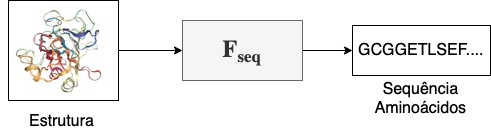
\includegraphics[width=.8\textwidth]{figuras/metodologia-SeqDes.jpg}
\end{figure}

%\subsection{Sequence Design baseado em busca}
\unnumberedsubsection{Sequence Design baseado em busca}

No \textit{Sequence Design} baseado em busca, 
a função $F_{seq}$ é definida por um processo iterativo. 
Inicialmente, uma sequência de aminoácidos é gerada com base em uma heurística inicial $H$.
Essa sequência é então avaliada por uma função objetivo $F_{obj}$, 
responsável por calcular a métrica a ser otimizada.
A cada iteração, 
a nova sequência gerada é comparada com a sequência anterior de acordo com a métrica definida. 
Se a sequência atual apresentar melhor desempenho, o Agente $A$ a define como nova sequência final.
Caso contrário, a sequência final é mantida. 
Em ambos os cenários, o próximo passo é a aplicação de uma mutação pelo Agente $A$ sobre 
a sequência atual com o objetivo de explorar novas possibilidades no espaço de busca.
Esse processo é repetido até que um critério de parada seja atingido, 
como um número máximo de iterações ou a convergência da métrica calculada por $F_{obj}$.


\begin{figure}[H]
  \centering
  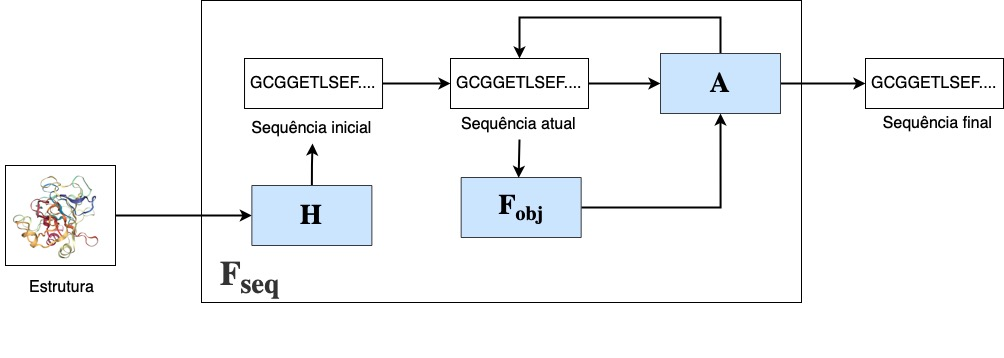
\includegraphics[width=.8\textwidth]{figuras/metodologia-SearchBased.jpg}
  \caption[\textit{Sequence Design} baseado em busca]{\textit{Sequence Design} baseado em busca define $F_{seq}$ 
           como um processo iterativo que combina uma 
           heurística inicial $H$, a avaliação por $F_{obj}$ e as modificações realizadas pelo Agente $A$. 
           O processo é repetido até atingir um número máximo de iterações ou um limiar calculado por $F_{obj}$.}
  \label{fig:seqdes_search_based}
\end{figure}

O software \textit{Rosetta} (\cite{Rosetta}) é uma das ferramentas 
mais amplamente utilizadas para otimização e \textit{design} de proteínas.
Ele implementa um \textit{pipeline} iterativo que combina heurísticas de geração de sequências iniciais, 
avaliações de estabilidade estrutural e técnicas de mutação orientada para explorar o espaço de sequências.
Em seu \textit{pipeline}:


\begin{itemize}
    \item \textbf{Heurística inicial ($H$):}  
    Utiliza a sequência de uma proteína estruturalmente semelhante como ponto de partida.

    \item \textbf{Função objetivo ($F_{obj}$):}  
    Avalia a energia livre da proteína resultante, considerando fatores como interações de Van der Waals,
    interações eletrostáticas e ligações de hidrogênio.

    \item \textbf{Agente ($A$):}  
    Utiliza o Método de Monte Carlo (MMC) para introduzir mutações na sequência e aceitar novas configurações com menor energia livre,
    guiando iterativamente o processo de otimização.
\end{itemize}

Abordagens alternativas podem usar a similaridade estrutural como função objetivo,
sendo uma métrica amplamente utilizada o \textit{Template Modeling Score} (TMScore) (\cite{tmscore}).

%\subsection{\textit{Sequence Design} baseado em Aprendizado Profundo}
\unnumberedsubsection{Sequence Design baseado em Aprendizado Profundo}
\textit{Sequence Design} baseado em aprendizado profundo define a função $F_{seq}$ 
a partir de redes neurais artificiais. 
Pesquisas como o \cite{ProteinMPNN} por exemplo, 
determina a $F_{seq}$ como uma rede neural profunda, denominada \textit{ProteinMPNN}, 
que mapeia de forma direta a estrutura alvo à sequência de aminoácidos. 
A rede é construída através de uma \textit{Message Passing Neural Network} (MPNN) 
composta por uma arquitetura \textit{encoder-decoder} 
que se baseia nas características da estrutura como distância e orientação dos átomos no espaço 
para fazer predições (\cite{ProteinMPNN}). 

\begin{figure}[H]
  \centering
  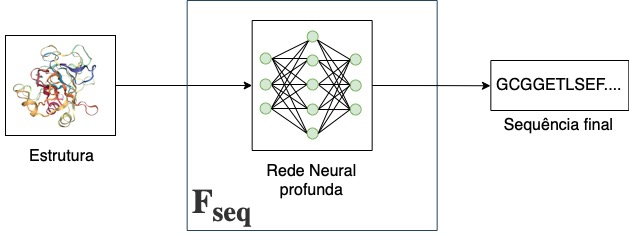
\includegraphics[width=.8\textwidth]{figuras/metodologia-DeepLearningBased.jpg}
  \caption{\textit{Sequence Design} baseado em aprendizado profundo.}
\end{figure}

%\section{\textit{Sequence Design} baseado em Aprendizado por Reforço Profundo} 
\unnumberedsection{\textit{Sequence Design} baseado em Aprendizado por Reforço Profundo}
\label{section:Proposta}

Além de suscitar uma possível resposta imunológica, 
o tratamento da hemofilia tipo B baseado na infusão de  FIX
é custoso devido ao pouco tempo de vida da proteína na corrente sanguínea, demandando infusões frequentes. 
Neste sentido, este trabalho busca responder à seguinte pergunta científica: 
É possível, através de \textit{Sequence Design}, projetar uma proteína que desempenhe a mesma função do FIX, 
mas com maior estabilidade, menor imunogenicidade e menos necessidade de infusões?

Para responder a esta questão, formulamos a hipótese de que, 
se existir uma proteína alternativa superior ao FIX, 
ela deverá ser estruturalmente similar. 
Assim, o objetivo será identificar proteínas estruturalmente semelhantes que atendam aos critérios estabelecidos.
Para simplificar o problema, focaremos no projeto do domínio protease, 
reconhecido como o mais relevante para a função do FIX (\cite{FIX}).

Nossa dissertação consiste no desenvolvimento de um \textit{pipeline} que combina estratégias de busca 
com aprendizado profundo para otimização de sequências proteicas. 
Esse \textit{pipeline} será estruturado em três módulos principais: Condições Iniciais, 
Treinamento e Geração de Sequências.


O módulo de Condições Iniciais tem como objetivo obter a sequência inicial de aminoácidos 
por meio da heurística \( H \), além de calcular o erro inicial associado a essa sequência 
utilizando a função objetivo \( F_{\text{obj}} \). 
Para isso, empregaremos o \textit{ProteinMPNN} como heurística \( H \) 
e o TMScore como métrica de avaliação estrutural \( F_{\text{obj}} \).  

Diferente do uso de agentes que realizam mutações aleatórias, como no \textit{Rosetta},
no módulo de Treinamento treinaremos uma rede neural profunda, o \textit{GenSeq}, para atuar como o Agente $A$,
sendo capaz de realizar mutações que otimizem a similaridade com a estrutura alvo, isto é, o FIX.
O \textit{GenSeq} será treinado utilizando um algoritmo de Aprendizado por Reforço Profundo (DRL), 
o \textit{Proximal Policy Optimization} (PPO) (\cite{PPO}).

Por fim, no módulo de Geração de Sequências, 
o agente treinado será utilizado para produzir um conjunto de variantes proteicas estruturalmente semelhantes ao FIX,
por meio de um processo de mutação orientado. 
As sequências geradas serão então avaliadas para identificar possíveis candidatas viáveis 
que possam substituir o FIX no tratamento da hemofilia tipo B.

\begin{figure}[H]
  \centering
  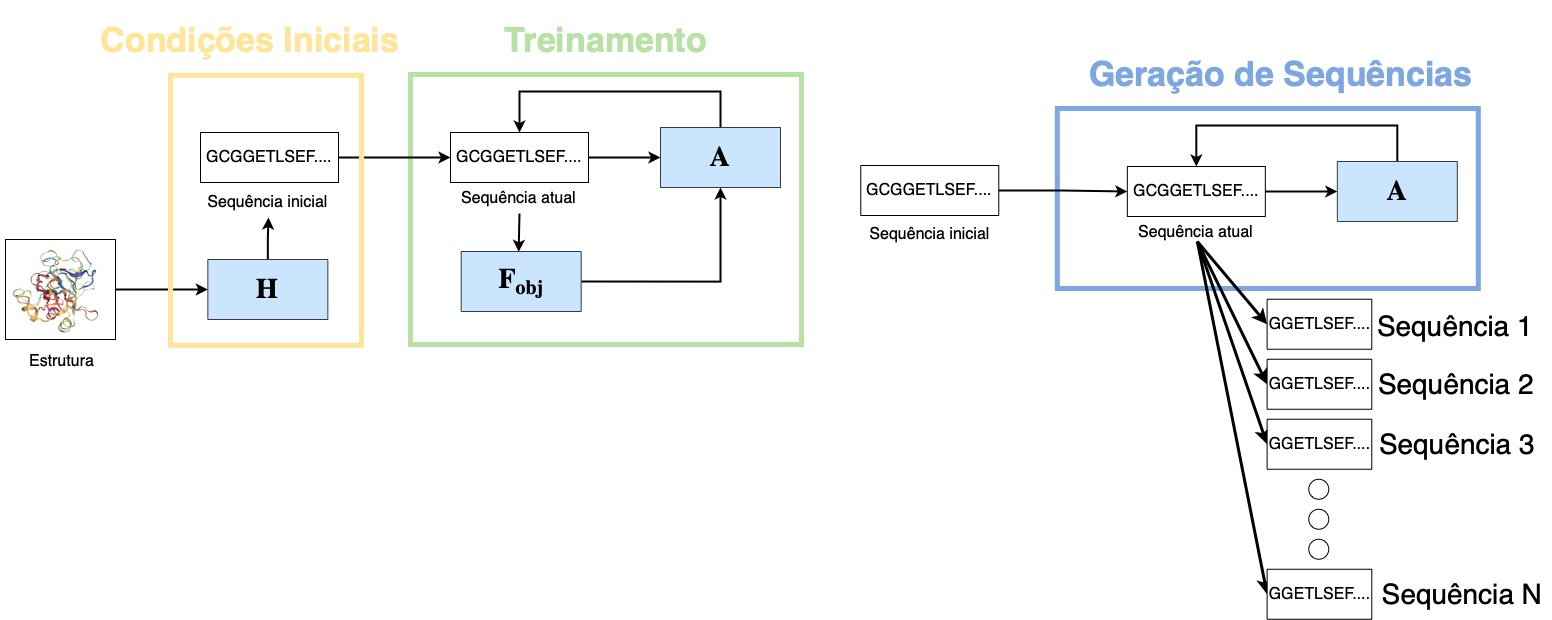
\includegraphics[width=.8\textwidth]{figuras/metodologia-pipeline_proposta.jpg}
  \caption{\textit{Pipeline} proposto de \textit{Sequence Design}.}
  \label{fig:proposta}
\end{figure}

%\section{Objetivos}
\unnumberedsection{Objetivos}

\begin{enumerate}
  \item Obter um conjunto de sequências de aminoácidos que mimetizem a estrutura do FIX baseado na métrica TMScore.
  \item Avaliar, dentro do conjunto de proteínas obtidas em 1, quais possuem potencial de substituir o FIX de modo tornar o tratamento de Hemofilia tipo B mais acessível e eficiente.
  \item Desenvolver um \textit{pipeline} genérico que produza sequências que mimetizem uma estrutura qualquer.
\end{enumerate}

%\section{Contribuições}
\unnumberedsection{Contribuições}
As contribuições deste trabalho são:
\begin{enumerate}
  \item O desenvolvimento de proteínas potenciais candidatas a substituir o FIX no tratamento da hemofilia tipo B.
  \item Um \textit{pipeline} para \textit{Sequence Design} baseado em Aprendizado por Reforço Profundo, que pode ser adaptado para outras proteínas com estruturas conhecidas.
  \item Introdução da métrica IMI (Imuno Índice), que quantifica a propensão de uma proteína gerar uma resposta imunológica adversa.
  \item O artefato do modelo de aprendizado por reforço profundo, o \textit{GenSeq}, que pode ser utilizado para geração de novas sequências proteicas a partir da estrutura do FIX (\cite{repo}).
  \item O código fonte das implementações e os scripts utilizados para o treinamento do \textit{GenSeq}, bem como a avaliação 
  de similaridade estrutural, \textit{docking} e imunogenicidade das sequências geradas (\cite{repo}).
  \item Os arquivos PDB utilizados como entrada para o treinamento do \textit{GenSeq} e para a avaliação das proteínas geradas (\cite{repo}).
  \item Apresentação dos resultados no \textit{World Federation of Hemophilia (WFH) 2024}, realizado em Madrid, Espanha, por meio do pôster científico intitulado \textit{“Protein Design and Deep Learning: A New Frontier in Hemophilia B Management”} \cite{WFH2024}
\end{enumerate}

\chapter{Revisão Bibliográfica}
\label{subsection:structure_pred}

O objetivo deste capítulo é situar o presente trabalho no contexto das contribuições existentes na área de pesquisa.
Para isso, analisamos diversas publicações da literatura que estão alinhadas com os objetivos deste estudo.


\section{Trabalhos relacionados}
% Tratamentos Atuais para Hemofilia B  
O tratamento atual para hemofilia B baseia-se na reposição do FIX por meio de proteínas recombinantes ou derivadas do plasma humano. 
A introdução de fatores de coagulação recombinantes na prática clínica representou um marco no manejo da doença, 
proporcionando maior segurança e eficácia em comparação com derivados do plasma, 
reduzindo significativamente os riscos de transmissão de patógenos (\cite{COHEN1995675}).  
No entanto, as terapias baseadas na reposição de FIX ainda apresentam desafios substanciais.
Devido à curta meia-vida do FIX na circulação, 
pacientes geralmente necessitam de infusões frequentes para manter níveis terapêuticos adequados,
o que aumenta os custos e a complexidade do tratamento (\cite{Mancuso}). 
Além disso, os pacientes podem desenvolver inibidores, 
que são anticorpos neutralizantes dirigidos contra o FIX,
comprometendo a eficácia do tratamento (\cite{Mancuso2}).
Avanços recentes, como o desenvolvimento de variantes do FIX de longa duração como o rFIX-Fc, 
estenderam a meia-vida da proteína, reduzindo a frequência de infusões (\cite{Massimo}). 
Apesar disso, essas terapias continuam a ser custosas e, em alguns casos,
limitadas pela resposta imunológica do paciente.  


% Design de Proteínas  
O design de proteínas surge como uma alternativa com potencial de desenvolver tratamentos mais eficientes. 
Trata-se de um campo emergente que busca criar ou modificar proteínas para otimizar suas funções biológicas, 
estabilidade estrutural ou características terapêuticas. 
Os avanços nessa área têm sido impulsionados pelo aprimoramento de tecnologias de modelagem molecular
e pelo uso de ferramentas computacionais especializadas.
O software Rosetta (\cite{Rosetta}) por exemplo,
foi uma das primeiras ferramentas amplamente utilizadas para predição de estruturas proteicas.
Seu funcionamento baseia-se na minimização da energia livre de uma proteína, 
modelando interações moleculares fundamentais como interações de Van der Waals,
forças eletrostáticas, ligações de hidrogênio e efeitos hidrofóbicos.
A predição estrutural utilizando o Rosetta fundamenta-se no princípio de que a conformação nativa de uma proteína 
corresponde a conformação de menor energia livre. 
O processo é iterativo e inicia-se com a geração de modelos estruturais iniciais, 
frequentemente por meio da montagem de fragmentos, 
em que pequenos segmentos estruturais de proteínas conhecidas são recombinados para gerar conformações aproximadas da proteína alvo.
Para cada modelo gerado é estimado a energia livre da conformação.
A partir dessas estimativas, o Rosetta aplica métodos estocásticos, 
como Monte Carlo Simulated Annealing, para explorar diferentes conformações e minimizar a função de energia,
conduzindo a um refinamento progressivo da estrutura modelada. 
Os modelos que apresentam menores valores são considerados candidatos mais prováveis para representar a estrutura nativa
da proteína em estudo.


\cite{Alphafold2} introduziu o \textit{AlphaFold}, um modelo que
representou um avanço significativo na predição estrutural de proteínas,
ao introduzir uma abordagem baseada em \textit{deep learning} que superou 
métodos computacionais tradicionais.
O problema da predição estrutural pode ser formalmente descrito como a minimização da função de energia livre associada 
à conformação da proteína. Diferentemente dos métodos tradicionais que exploram o espaço conformacional por meio de amostragem estocástica,
o \textit{AlphaFold} aprende diretamente um mapa de distâncias e ângulos que minimiza essa função de energia.  
O modelo utiliza redes neurais treinadas em bancos de dados contendo estruturas proteicas determinadas experimentalmente, 
como as obtidas por cristalografia de raios X, espectroscopia por ressonância magnética nuclear (RMN) e criomicroscopia eletrônica. 
A base teórica do \textit{AlphaFold} fundamenta-se na 
modelagem das interações residuais a partir de alinhamentos múltiplos de sequências (MSA, Multiple Sequence Alignments) 
e do aprendizado das representações espaciais dos resíduos por meio de camadas de atenção baseadas em grafos.
O modelo recebe como entrada uma sequência de aminoácidos e gera um conjunto de representações internas (\textit{embeddings})
que capturam informações sobre a proximidade e orientação relativa dos resíduos na estrutura tridimensional da proteína.
O modelo foi amplamente validado por meio de sua participação na 
edição 14 do \textit{CASP (Critical Assessment of Structure Prediction)}, 
uma avaliação que compara métodos de predição de estrutura proteica com dados experimentais inéditos. 
No CASP14, o \textit{AlphaFold} demonstrou um desempenho quase equivalente ao de técnicas experimentais.
Esse avanço revolucionou o campo da biologia estrutural,
reduzindo a dependência exclusiva de métodos experimentais e abrindo novas possibilidades para a engenharia de proteínas
 e a compreensão de doenças associadas a dobramentos proteicos anômalos.


\cite{ESMFold} apresentaram o \textit{ESMFold}, 
um modelo baseado em \textit{transformers} capaz de realizar a predição de estruturas proteicas diretamente 
a partir de sequências de aminoácidos. 
Diferentemente de modelos como o \textit{AlphaFold},
que fazem uso extensivo de alinhamentos múltiplos de sequências (\textit{MSA, Multiple Sequence Alignments}) e atenção
baseada em grafos para inferir interações residuais,
o \textit{ESMFold} prioriza a velocidade de processamento, permitindo uma predição rápida de estruturas com precisão moderada.  
A arquitetura do \textit{ESMFold} baseia-se no modelo de linguagem proteica \textit{ESM-2}, 
um \textit{transformer} pré-treinado em grandes bancos de dados de sequências biológicas. 
Esse modelo aprende representações internas que capturam informações evolutivas e estruturais implícitas,
sem depender explicitamente de \textit{MSAs}. 
A predição estrutural ocorre por meio da inferência direta da topologia tridimensional da proteína a partir dessas representações,
minimizando a necessidade de computação intensiva e permitindo um tempo de inferência reduzido.
Embora o \textit{ESMFold} não alcance a precisão estrutural do \textit{AlphaFold},
sua abordagem é extremamente vantajosa para aplicações que exigem triagem de alto desempenho,
como análises em larga escala e estudos preliminares de modelagem proteica. 
Sua rapidez permite que estruturas sejam geradas em segundos, 
enquanto o \textit{AlphaFold} pode demandar minutos a horas,
dependendo da complexidade da proteína analisada. 

Ferramentas como o \textit{ProteinMPNN} \cite{ProteinMPNN} utilizam arquiteturas baseadas em \textit{Message Passing Neural Networks} 
(MPNNs) para prever sequências de aminoácidos capazes de adotar conformações tridimensionais específicas.
Diferentemente dos métodos tradicionais de \textit{design} de proteínas, 
que frequentemente utilizam abordagens estocásticas ou heurísticas para otimizar sequências, como o \textit{Rosetta},
o \textit{ProteinMPNN} emprega \textit{deep learning} para explorar de maneira eficiente o espaço de sequências
e gerar variantes estruturalmente viáveis.  
O modelo opera sobre a representação estrutural de uma proteína como um grafo,
onde os resíduos de aminoácidos correspondem a nós e as interações entre eles são representadas por arestas ponderadas. 
A passagem de mensagens ocorre entre os nós vizinhos, permitindo que o modelo aprenda padrões de interações residuais 
que favorecem a estabilidade estrutural da proteína. 
O modelo consiste de 3 camadas de \textit{encoder} e 3 de \textit{decoder} seguidos de uma camada escondida de 128 neurônios 
prevendo a sequência de aminoácidos de modo auto regressivo, do terminal N ao C. 



\cite{DyNAPPO} apresentaram o \textit{DyNA PPO}, que consiste em uma
abordagem de \textit{desing} de sequências proteicas baseada em aprendizado por reforço profundo (\textit{Deep Reinforcement Learning}, DRL),
atualizando seus parâmetros através do algorítimo \textit{Proximal Policy Optimization}, PPO.  
O \textit{DyNA PPO} modela o problema do design de proteínas como um processo de decisão de Markov, 
onde um agente gera sequências de aminoácidos de forma autoregressiva, 
adicionando resíduos um por um. 
A função de recompensa é baseada em métricas de estabilidade estrutural e funcionalidade da proteína, 
sendo calculada apenas ao final da geração da sequência. 
Esse mecanismo permite que o modelo aprenda estratégias eficazes para explorar o espaço de sequências de forma eficiente.  
O modelo é treinado iterativamente, ajustando sua política para maximizar a recompensa acumulada.
Durante o treinamento, um conjunto de redes neurais auxiliares avalia a qualidade das sequências geradas,
fornecendo sinais de aprendizado ao agente. 
Embora o \textit{DyNA PPO} tenha demonstrado resultados promissores em benchmarks computacionais, 
sua validação experimental ainda está em aberto. 

A análise da literatura existente evidencia que o design computacional de proteínas tem avançado significativamente, 
impulsionado por metodologias como modelagem molecular baseada em física, aprendizado profundo e aprendizado por reforço. 
Modelos como \textit{AlphaFold}, \textit{Rosetta}, \textit{ESMFold} e \textit{ProteinMPNN} têm contribuído de forma expressiva
para a predição estrutural e o \textit{design} de sequências proteicas.
Além disso, técnicas de aprendizado por reforço, como \textit{DyNA PPO}, 
demonstraram grande potencial para a otimização de sequências proteicas, 
explorando o espaço conformacional de maneira adaptativa e eficiente.  

No entanto, não foram encontrados estudos que apliquem aprendizado 
por reforço especificamente para a otimização do FIX no tratamento da hemofilia B. 
A pesquisa realizada não identificou publicações que abordem a aplicação dessa abordagem para modificar ou aprimorar a sequência do FIX,
de modo a aumentar sua estabilidade, prolongar sua meia-vida ou reduzir sua imunogenicidade como proposto pelo presente trabalho. 

\chapter{Fundamentação teórica}

Neste capítulo vamos apresentar os fundamentos teóricos utilizados neste trabalho acerca de proteínas e aprendizado por reforço profundo. 


\section{Proteína}
Uma proteína é uma macromolécula biológica composta por cadeias de aminoácidos. 
Constituem a maior parte da massa seca de uma célula, podendo desempenhar funções enzimáticas, estruturais,
imunológicas, de transporte, entre outras (\cite{Bio}). 

Existem milhares de proteínas diferentes em uma célula,
onde cada uma é composta por uma sequência distinta dos 20 tipos de aminoácidos encontrados na natureza,
unidos através de ligações peptídicas.
Por conta disto, as proteínas são também conhecidas como polipeptídeos (\cite{Bio}). 

A cadeia polipeptídica é composta por três componentes: a cadeia principal,
as cadeias laterais e as ligações peptídicas.
A cadeia principal é também referida como o esqueleto da proteína e
é definida como uma série repetitiva e encadeada de átomos de carbono,
nitrogénio e oxigénio. Anexadas a cadeia principal, encontram-se as cadeias laterais. 
Estas não estão envolvidas nas ligações peptídicas e são responsáveis por caracterizar as principais propriedades da proteína \cite{Bio}. 

\begin{figure}[H]
     \centering
     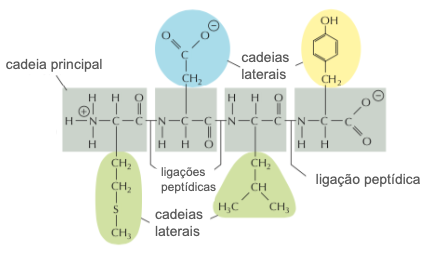
\includegraphics[width=0.6\textwidth]{figuras/ProteinBackbone.png}
     \caption{Componentes de uma proteína}
\end{figure}

\begin{figure}[H]
     \centering
     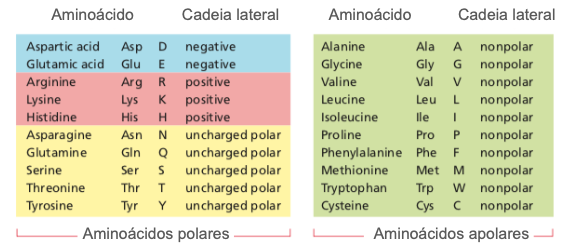
\includegraphics[width=0.7\textwidth]{figuras/20Aminoacidos.png}
     \caption[Aminiácidos]{Cada aminoácido tem uma abreviação de uma ou três letras - figura 3-2 adaptada \cite{Bio}.}
\end{figure}


\subsection{Estrutura proteíca}

A função de uma proteína está intimamente relacionada à sua estrutura tridimensional,
que é formada principalmente a partir das interações entre as cadeias laterais e móleculas encontradas no meio físico ao qual
a proteína está inserida. Devido a essas interações, a maioria das proteínas assume uma estrutura tridimensional única,
que é determinada pela ordem dos aminoácidos na sequência. 
A conformação final tende a ser aquela que possui a menor energia livre (\cite{Bio}).
Por energia livre entende-se como à energia potencial total do sistema molecular que inclui a proteína e seu meio circundante. 
Essa energia é uma medida termodinâmica que combina componentes de energia entálpica (relacionada a ligações químicas e interações eletrostáticas) 
e entropia (relacionada à desordem ou ao número de configurações possíveis das moléculas).

\cite{Bio} explica que a polaridade das cadeias laterais desempenham um papel importante na predição estrutural da proteína. 
As cadeias não polares (hidrofóbicas) tendem a se agrupar no interior da molécula, 
evitando contato com a água. 
Já as polares tendem a se dispor perto da superfície da molécula,
onde podem formar ligações de hidrogênio com a água e outras moléculas polares. 

\begin{figure}[H]
     \centering
     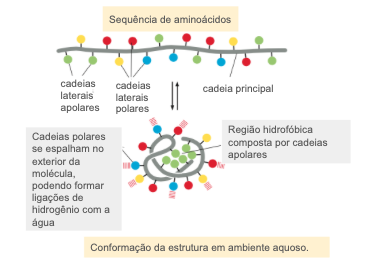
\includegraphics[width=0.6\textwidth]{figuras/ConformacaoProteica.png}
     \caption[Exemplo de conformação protéica]{Exemplo de conformação protéica \cite{Bio} - adaptado}
     %\label{Label de referência para a imagem}
\end{figure}


\subsection{O Fator IX}
\label{subsection:FIX} 
O Fator IX (FIX) é uma proteína essencial para o processo de coagulação.
Quando ativado (FIXa), atua em conjunto com o Fator VIIIa (FVIIIa) para formar 
um complexo conhecido como tenase intrínseco, que é responsável por ativar o Fator X. 
Este processo é fundamental para a geração de trombina e formação de coágulos (\cite{FIX}). 
A ausência ou disfunção do FIX compromete o processo de ativação do FX,
impossibilitando uma coagulação saúdavel, o que configura a hemofilia tipo B.

\begin{figure}[H]
    \centering
    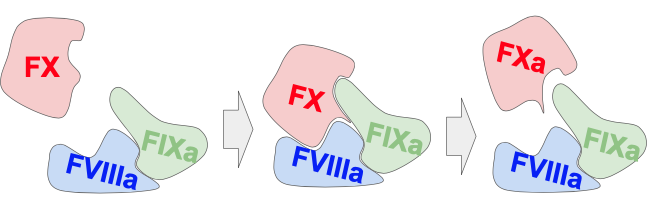
\includegraphics[width=.8\textwidth]{figuras/ativaFX.png}
    \caption{Atuação do FIXa na ativação do FX}
  \end{figure}

O FIXa é composto por diferentes domínios,
cada um desempenhando um papel essencial nas interações moleculares que permitem a formação do complexo tenase intrínseco. 
Na região N-terminal, o domínio Gla (gamma-carboxiglutâmico) é responsável por ligar o FIXa a superfícies de membranas fosfolipídicas, 
uma interação dependente de íons de cálcio, 
fundamental para posicionar o complexo de coagulação no local da lesão vascular (\cite{FIX}). 
Os domínios de fator de crescimento epidérmico (EGF1 e EGF2) desempenham funções complementares: 
o EGF1 facilita o reconhecimento de cofatores e substratos, enquanto o EGF2 interage com o domínio A3 do Fator VIIIa,
contribuindo para a montagem do complexo tenase (\cite{FIX}). 
O papel mais crítico para a estabilidade e a funcionalidade do complexo tenase reside no domínio protease,
cuja interação com o domínio A2 do FVIIIa permite a ativação conformacional necessária para uma catálise eficiente do FX.
%O domínio protease de serina contém o sítio ativo responsável pela atividade catalítica do FIXa, 
%interagindo diretamente com os domínios A2 e A3 do FVIIIa \cite{FIX}. Por conta disso,
%o domínio protease de serina é o mais relevante para a estabilidade e a eficiência catalítica do 
%complexo tenase intrínseco. 
\cite{FIX} explica que variantes do FIXa, como o FIX-Padua, que modificam o domínio protease, 
apresentam maior eficiência catalítica, destacando seu papel central no desenvolvimento de proteínas otimizadas para terapia de hemofilia.

%A formação de um complexo tenase estável depende de várias interações específicas.
%O domínio Gla do FIXa se liga ao domínio C2 do FVIIIa, promovendo a ancoragem na membrana fosfolipídica.
%Os domínios EGF1 e EGF2 interagem com os domínios A1 e A3 do FVIIIa, conferindo estabilidade adicional ao complexo.
%O papel mais crítico para a estabilidade e a funcionalidade do complexo tenase reside no domínio protease,
%cuja interação com o domínio A2 do FVIIIa permite a ativação conformacional necessária para uma catálise eficiente do FX.

\begin{figure}[H]
    \centering
    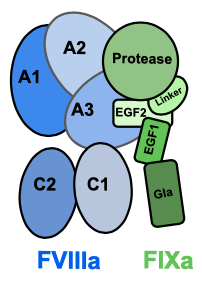
\includegraphics[width=.3\textwidth]{figuras/FIXa_FVIIIa.png}
    \caption[Interação entre FIXa e FVIIIa]{Interação entre FIXa e FVIIIa, formando o complexo tenase. Adaptação da figura 3 de \cite{FIX}}
  \end{figure}

A estrutura do domínio protease é a estrutura alvo do \textit{pipeline} de \textit{sequence design} proposto por este trabalho.  
É composta por 235 resíduos. 
Logo, o espaço de possíveis novas sequências com este tamanho, considerando 20 diferentes aminoácidos, é de $235^{20}$. 

\begin{figure}[H]
    \centering
    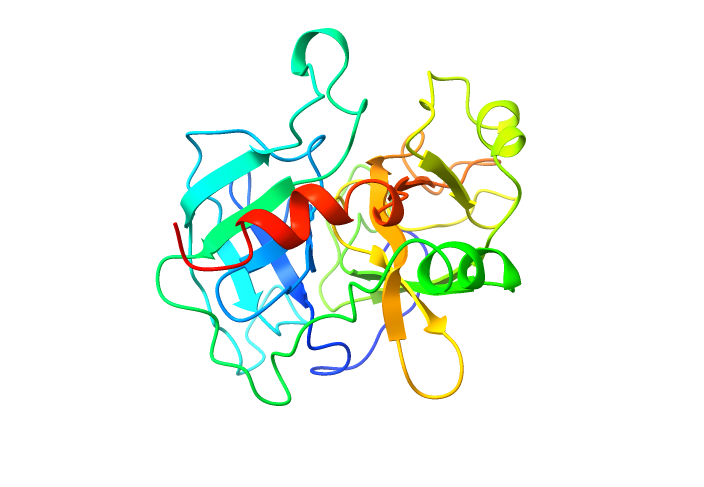
\includegraphics[width=.6\textwidth]{figuras/FIX.jpg}
    \caption{Estrutura alvo - Domínio protease do Fator IXa}
  \end{figure}

As proteínas projetadas neste estudo serão desenvolvidas para mimetizar a estrutura do domínio protease.
O objetivo é identificar, entre as variantes geradas, aquelas capazes de estabelecer interações mais estáveis com o FVIIIa,
aprimorando a estabilidade do complexo tenase intrínseco. 
Adicionalmente, espera-se que as novas estruturas apresentem um perfil imunogênico reduzido em comparação ao FIXa nativo, 
contribuindo para maior segurança e eficácia terapêutica.

\subsection{Docking}
\label{subsection:Docking} 
A análise de \textit{docking} é uma técnica computacional amplamente utilizada no estudo de interações biomoleculares,
particularmente para prever a orientação e a afinidade entre duas moléculas,
como proteínas. Nesse sentido, é essencial para avaliar como uma proteína substituta do FIXa interage com o FVIIIa. 
O \textit{docking} molecular simula o reconhecimento entre uma molécula receptora e outra ligante. 
No caso de interações proteína-proteína, o receptor e o ligante são ambos macromoléculas,
cujas superfícies e conformações influenciam a formação de um complexo estável.
O objetivo do \textit{docking} é identificar as poses mais favoráveis termodinamicamente, ou seja, 
aquelas que minimizam a energia livre do sistema.

Durante o \textit{docking}, diversas poses do ligante em relação ao receptor são geradas.
Ferramentas como RosettaDock ou AutoDock realizam essa busca, explorando translações, rotações e flexibilidade local.
Cada pose é avaliada com base em métricas energéticas, como a \textit{Contact Molecular Surface} (CMS), \textit{Interface Buried SASA} (IBSASA),
\textit{Delta Gibbs Free Energy of Binding} (DDG) e \textit{Spatial Aggregation Propensity Score} (SAP Score).

A CMS é uma medida desenvolvida para superar as limitações de métricas tradicionais, 
como \textit{Shape Complementarity} (SC) e \textit{Delta Solvent Accessible Surface Area} (Delta SASA) \cite{Docking}.
Enquanto SC analisa a complementaridade geométrica entre superfícies moleculares e 
Delta SASA calcula a área de superfície acessível ao solvente antes e depois da complexação,
ambas possuem limitações na identificação de interfaces bem empacotadas (\cite{Docking}).
Em contraste, o CMS combina a área de contato com um fator de penalização baseado na distância entre triângulos de superfície,
oferecendo uma representação mais precisa da qualidade do empacotamento na interface (\cite{Docking}).

A IBSASA é frequentemente usada para estimar a extensão de área de superfície enterrada durante a formação de um complexo proteico,
correlacionando-se com a estabilidade de ligação. 
No entanto, sozinha, essa métrica pode ser enganosa em interfaces mal organizadas, 
onde grandes áreas de contato podem não resultar em interações eficazes (\cite{Docking}). 

Por outro lado, a DDG fornece uma medida direta do quão favorável energéticamente é uma interação,
com valores mais negativos indicando maior estabilidade termodinâmica (\cite{Docking}). 
A DDG, calculada frequentemente com o software Rosetta, 
permite a otimização de sequências e conformações para maximizar a energia de ligação.

Por fim, o SAP Score avalia a presença de regiões hidrofóbicas expostas na superfície da proteína, 
utilizando a área de superfície acessível ao solvente (SASA) como referência. 
A partir dessa análise, estima-se a propensão da proteína ou do complexo formado à agregação indesejada.
Valores mais baixos de SAP indicam menor exposição de patches hidrofóbicos ao solvente,
sugerindo maior estabilidade estrutural e menor risco de agregação, o que é desejável na formação de complexos moleculares estáveis
(\cite{Docking}).


%O design de proteínas substitutas do FIX depende diretamente da eficácia dessas proteínas em formar complexos estáveis
%e funcionais com o FVIII. 
%A análise de docking não só ajuda a identificar mutações promissoras no FIX artificial,
%mas também fornece insights sobre como melhorar sua funcionalidade na cascata de coagulação.



\subsection{Resposta Imunológica}
\label{subsection:RespImuno} 

A resposta imune desencadeada por uma proteína terapêutica é um fator crítico 
que pode influenciar diretamente sua segurança e eficácia. 
No contexto de \textit{sequence design} de uma proteína substituta do FIXa,
a análise dessa resposta imune é especialmente relevante para evitar complicações associadas à formação de inibidores,
uma limitação comum no tratamento de hemofilia. 
Esses inibidores são anticorpos neutralizantes que se ligam à proteína administrada,
reduzindo sua eficácia e exigindo estratégias de tratamento alternativas mais caras e menos seguras.

A imunogenicidade está intrinsicamente relacionada à presença de epítopos imunogênicos na sequência da proteína. 
Esses epítopos são regiões específicas que se ligam a moléculas de MHC classe II em células 
que apresentam antígenos (APCs), 
facilitando a ativação de linfócitos T auxiliares (\cite{Imuno}). 
A afinidade de ligação é um fator determinante na indução da resposta imune. 
Altas afinidades entre peptídeos e MHC-II aumentam a probabilidade 
de reconhecimento imune e subsequente ativação de células T (\cite{Imuno}).

A predição de afinidade de ligação entre epítopos e MHC-II emprega ferramentas computacionais 
baseadas em aprendizado de máquina,
como o NetMHCIIpan, que simulam interações entre peptídeos derivados da proteína e uma variedade de alelos de MHC. 
A sequência da proteína é fragmentada em peptídeos sobrepostos com comprimentos típicos de 8 a 15 aminoácidos,
e a afinidade de cada peptídeo é quantificada por meio do valor de $IC_{50}$ (concentração inibitória de 50\%).
Peptídeos com valores de $IC_{50}$ baixos (($IC_{50}$ < 50 nM)) indicam maior afinidade de ligação e, portanto, 
são mais propensos a serem reconhecidos como epítopos imunogênicos (\cite{Imuno}).

Portanto, o objetivo ao projetar a proteína substituta do FIXa é não apenas otimizar a estabilidade de ligação ao FVIIIa, 
mas também evitar a apresentação de novos epítopos imunogênicos que poderiam levar à formação de inibidores. 
A redução da imunogenicidade melhora a adesão ao tratamento e reduz complicações, 
consolidando a importância da integração de predições imunológicas 
no \textit{pipeline} de desenvolvimento de proteínas terapêuticas.

%Apresentar equações/imagens ilustrativas das métricas

\subsection{Mutação}
Uma mutação no contexto de proteínas refere-se a uma modificação na sequência de aminoácidos. 
Por menor que seja esta modificação, a mutação pode acarretar em uma alteração na estrutura tridimensional da proteína,
uma vez que a ordem que os aminoácidos estão dispostos na sequência influencia diretamente na conformação da estrutura. 
Neste trabalho, vamos assumir que uma mutação consiste na substituição de apenas um aminoácido por outro na sequência. 

\subsection{Similariedade entre estruturas}
\label{subsection:TMScore}  
Para projetar proteínas semelhantes ao FIXa, é necessário definir uma métrica de similaridade entre estruturas.
Duas métricas amplamente utilizadas são o \textit{Root-Mean-Square Deviation} (RMSD) 
e o \textit{Template Modeling Score} (TMScore) (\cite{tmscore}),
cada uma com características próprias que influenciam sua adequação a diferentes cenários de comparação estrutural.

O \textbf{RMSD} é definido como a raiz quadrada da média dos quadrados das distâncias 
entre pares de átomos correspondentes em duas estruturas alinhadas:

\begin{equation}
    \text{RMSD} = \sqrt{\frac{1}{N} \sum_{i=1}^{N} d_i^2},
\end{equation}

\noindent Onde \(N\) representa o número de pares de átomos alinhados e \(d_i\) é a distância entre os \(i\)-ésimos átomos nas estruturas comparadas. 
Embora seja uma métrica intuitiva, o RMSD é altamente sensível a desalinhamentos locais e não é normalizado pelo comprimento da proteína,
o que limita sua eficácia ao comparar proteínas de diferentes tamanhos.

O \textbf{TMScore}, por sua vez,
mede a similaridade estrutural global, superando limitações do RMSD. \cite{tmscore} a formulou da seguinte maneira:

\begin{equation}
    \text{TMScore} = \frac{1}{L_{\text{ref}}} \sum_{i=1}^{L_{\text{model}}} \frac{1}{1 + \left(\frac{d_i}{d_0(L_{\text{ref}})}\right)^2},
\end{equation}

\noindent Onde \(L_{\text{ref}}\) é o número de resíduos na estrutura de referência,
 \(L_{\text{model}}\) é o número de resíduos no modelo comparado, 
 e \(d_i\) é a distância entre os átomos \(C_\alpha\) alinhados. 
 
 \cite{tmscore} define \(d_0\) em função de \(L_{\text{ref}}\) da seguinte maneira:

\begin{equation}
    d_0(L_{\text{ref}}) = 1.24 \times (L_{\text{ref}} - 15)^{1/3} - 1.8.
\end{equation}

Este parâmetro adapta a escala de distâncias consideradas significativas para o alinhamento estrutural,
ajustando-se ao comprimento da proteína de referência, \( L_{\text{ref}} \). 
O termo \( (L_{\text{ref}} - 15)^{1/3} \) 
reflete uma relação empírica entre o tamanho da proteína e as distâncias típicas entre resíduos alinhados,
modelando o crescimento da distância permissível conforme a proteína aumenta de tamanho.
A constante multiplicativa 1.24 e o deslocamento -1.8 também foram determinados empiricamente para fornecer 
um valor de \( d_0 \) que otimiza a correlação entre o TMScore e a percepção biológica de similaridade estrutural.
Essa função adapta o limiar de normalização das distâncias entre pares de resíduos alinhados,
garantindo que proteínas de diferentes comprimentos sejam comparadas de forma justa.
Proteínas maiores toleram distâncias absolutas maiores entre resíduos alinhados sem que o TMScore seja severamente penalizado (\cite{tmscore}).
 

O \textit{TMScore} varia entre 0 e 1, onde valores próximos a 1 indicam alta similaridade topológica (\cite{tmscore}).
Se a distância entre cada par alinhado de átomos \(C_\alpha\) for igual a 0, então o TMScore é igual a 1, indicando sobreposição completa 
entre as macromoléculas. Em contra partida, quanto maiores são as distâncias, menor é o TMScore (mais próximo de 0).

Devido à sua robustez na avaliação da similaridade estrutural global e à sua interpretabilidade,
com valores limitados entre 0 e 1, adotaremos o TMScore como a métrica principal a ser otimizada neste projeto.
O cálculo desta medida será feito a partir da plataforma \textit{US-align} desenvolvida por (\cite{USalign}).


\subsection{Conservation Score}
\label{subsection:CS}
O \textit{Conservation Score} (CS) é uma métrica que estima a importância ou 
contribuição individual de cada resíduo da sequência na caracterização da estrutura da proteína.
Resíduos cruciais na estrutura da proteína tendem a ser conservados,
visto que alterações neles podem impactar significativamente a função proteíca (\cite{CS}). 
O \textit{score} é obtido levando-se em conta a frequência com que certas combinações de aminoácidos 
ocorrem em proteínas homólogas ao longo da evolução das espécies (\cite{Eddy}). 
Para este trabalho, utilizamos o CS calculado pelo servidor ConsurfDB (\cite{ConsurfDB}),
tendo a estrutura do FIXa de coagulação como entrada. 

\begin{figure}[H]
    \centering
    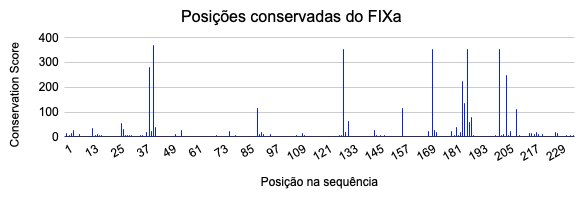
\includegraphics[width=.8\textwidth]{figuras/ConservationScore.png}
    \caption[FIXa Conservation Score]{A maior parte dos resíduos do FIXa possuem um baixo CS. Os maiores valores estão concentrados em cerca de 12 resíduos 
    espalhados ao longo da sequência.}
  \end{figure}

A identificação de posições conservadas é um aspecto fundamental ao projetar novas proteínas,
pois fornece informações essenciais para evitar mutações em regiões críticas,
preservando assim a estabilidade estrutural e a função biológica da molécula.

\subsection{Similariedade entre aminoácidos}
\label{subsection:AminoDist}
Da mesma forma que regiões com altos score de conservação devem ser evitadas, 
convém evitar mutações que substituem aminoácidos muito diferentes.
Nesse sentido, para mensurar o nível de similaridade entre os aminoácidos,
utilizamos uma métrica de distância fundamentada no trabalho de \cite{aminodist}, 
que propõe uma abordagem vetorial para representar as propriedades de cada aminoácido.
Nesse estudo, cada aminoácido foi descrito por um vetor de 544 dimensões, 
incorporando uma ampla gama de características físico-químicas e estruturais. 
A construção desses vetores foi realizada com o auxílio do pacote seqinR (\cite{seqinR}), 
uma ferramenta especializada em análise de sequências biológicas.
O pacote seqinR utiliza uma base de dados abrangente contendo propriedades como peso molecular,
hidrofobicidade, polaridade, acessibilidade à superfície, entre outras,
para derivar descritores numéricos que caracterizam as propriedades de cada aminoácido.

A partir dessa representação, \cite{aminodist} introduziu
uma matriz de distâncias, construída a partir das distâncias euclidianas de cada par 
de vetores, fornecendo uma medida quantitativa da dissimilaridade entre aminoácidos.


\begin{figure}[H]
    \centering
    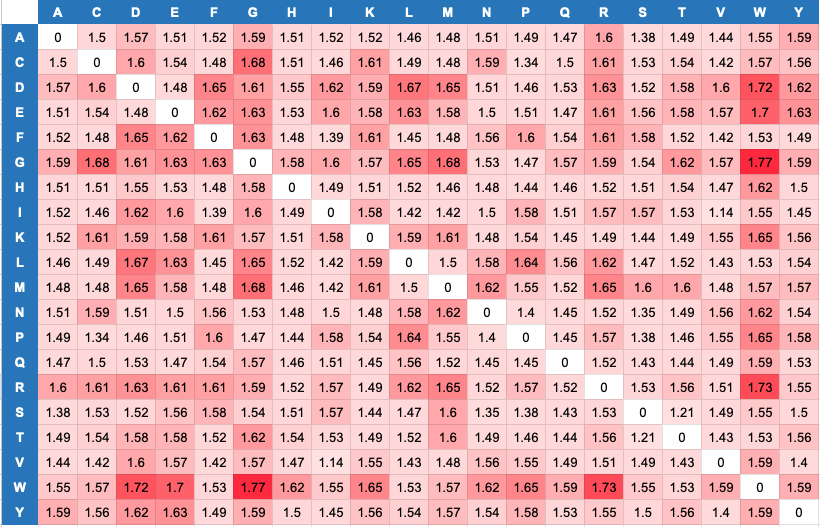
\includegraphics[width=.8\textwidth]{figuras/matrix_amino_dist.png}
    \caption[Distâncias entre aminoácidos]{Distâncias entre pares de aminoácidos \cite{aminodist}}
    \label{fig:matrixaminodist}
  \end{figure}


\section{Aprendizado por reforço profundo}
Nesta seção vamos introduzir os conceitos envolvidos no aprendizado por reforço profundo, que formam a base teórica da técnica que iremos utilizar: Proximal Policy Optimization (PPO). 
Para tal, será fornecido um contexto sobre Processo de Decisão de Markov (MDP), Redes Neurais (NN) e o método Ator-Crítico (AC). 


\subsection{Processo de Decisão de Markov}
O Processo de Decisão de Markov (MDP) é utilizado para modelar processos de forma probabilística. Ele é chamado de markoviano pois a distribuição de probabilidade de um estado depende apenas do estado anterior e da ação selecionada. Uma ação dá origem a um novo estado ao passo que promove alterações no estado atual. 
Um agente seleciona cada ação com base em uma política ($\pi$) que mapeia estados a ações. Em um MDP, o processo evolui em etapas, ou \textit{steps}, à medida que o agente toma ações. A sequência de estados, desde o inicial até o final, é chamada de episódio. A qualidade de cada ação é avaliada com base no quão benéfico é o estado alcançado.
De acordo com \cite{MDP}, o MDP pode ser definido como uma tupla 
<S,A,T,R> onde:

\begin{itemize}
   \item S é o conjunto de possíveis estados;
   \item A é o conjunto de ações que interferem no processo;
   \item T :S×A×S$\rightarrow$[0,1] é uma função que quantifica a probabilidade de mudança do estado s $\in$ S para o estado $s'$ $\in$ S, dado a ação a $\in$ A selecionada. É representado por T ($s'$ |s, a);
   \item r : S × A$\rightarrow$r é uma função que mede a recompensa por selecionar a ação a $\in$ A quando o processo está no estado s $\in$ S.
 \end{itemize}

De modo a encontrar uma boa política $\pi$, é necessário definir uma maneira de comparar diferentes políticas. Uma técnica comum é comparar a esperança da recompensa acumulada descontada, ou Valor de Retorno (R), que cada política produziu em um mesmo episódio.

\begin{equation}
    R = E\begin{bmatrix} \sum_{k=1}^{z} \gamma ^{k-1} r_k \end{bmatrix}
\end{equation}

\noindent
Sendo z o tamanho do episódio, k o índice do \textit{step} e o $r_k$ a recompensa obtida em k. A constante $\gamma$ é um valor entre 0 e 1, chamado de fator de desconto. Ele é responsável por atribuir um peso maior a recompensas obtidas no início do episódio. 

Além disso, existem outras duas métricas importantes para se avaliar a qualidade de uma política: a Função de Valor (V) e a função de Valor da Ação (Q). A primeira estima a vantagem de estar em um estado s, calculando a esperança de R dado o estado inicial s0 = s. 

\begin{equation}
    V_\pi(s) = E[R|s_0 = s]
\end{equation}

A segunda estima a vantagem de selecionar a ação $a$ estando no estado $s$. Em outras palavras, é definida como a esperança de R dado o estado inicial e a ação inicial:

\begin{equation}
    Q_\pi(s,a) = E[R|s_0 = s, a_0 = a]
\end{equation}


Neste trabalho vamos modelar tanto a política $\pi$ quanto a Função de Valor V utilizando redes neurais profundas. 

\subsection{Redes Neurais}
Inspirado no sistema neural humano, uma rede neural artificial consiste em um conjunto de nós, chamados de neurônios, interconectados por arestas (\cite{Bishop}). 
Em geral, é organizada em camadas, que incluem três tipos: a camada de entrada, a camada oculta e a camada de saída, conforme ilustrado na figura \ref{arqNN}.

\begin{figure}[H]
     \centering
     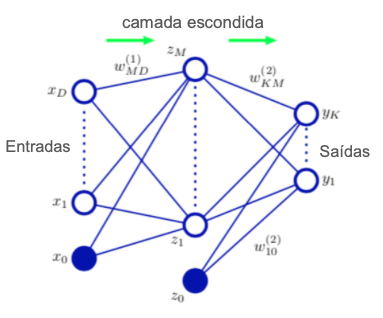
\includegraphics[width=0.6\textwidth]{figuras/RedeNeural.png}
     \caption[Arquitetura de rede neural]{Arquitetura de uma rede neural - \cite{Bishop} adaptado}
     \label{arqNN}
\end{figure}

Sinais fluem entre os neurônios através das arestas que estão associadas a um peso (w) que quantifica a sua importância. 
Nos neurônios é feito o processamento dos diversos sinais recebidos que, em seguida, aplica-se uma função, conhecida como função de ativação. 
Esta pode ser simplesmente uma combinação linear das entradas ponderadas pelos seus respectivos pesos, como pode ser função não linear como  sigmoid, 
tangente hiperbólica, entre outras (\cite{Bishop}).   

\begin{figure}[H]
     \centering
     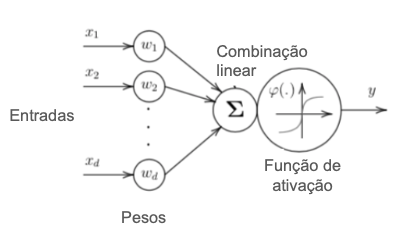
\includegraphics[width=0.6\textwidth]{figuras/ActivationFunc.png}
     \caption[Neurônio processando sinal]{Neurônio processando sinal \cite{Figueiredo}}
\end{figure}

Os pesos das arestas são ajustados durante a fase de treinamento,  de modo a orientar a rede a produzir a saída esperada para uma entrada específica. 
Nesta fase, é aplicado uma função de perda baseado na saída da rede. 
Existem diversas técnicas possíveis para minimizar a função de perda. 
Dentre elas, uma das mais tradicionais é a baseada no gradiente descendente, que atualiza os pesos conforme a equação a seguir. 

\begin{equation}
    w(t +1) = w(t) - n\nabla L(w(t)) 
\end{equation}

\noindent Onde w é o vetor de pesos, $n$ é uma constante positiva conhecida como taxa de aprendizagem, 
que quantifica o tamanho do ajuste dos parâmetros a cada iteração e $L$ é a função de perda. 
Um dos algoritmo mais utilizados para calcular o gradiente da função de perda e atualizar os parâmetros da rede é o \textit{Backpropagation} (\cite{Bishop}). 

No contexto deste trabalho, as funções de perda estarão fortemente relacionadas ao valor de Retorno R e a função de Valor V apresentadas na seção anterior. 


\subsection{Método Actor-Critic}

O método Ator-Crítico (AC) é um procedimento que tem como objetivo otimizar a política de um MDP (\cite{AC}). 
Ele é composto por dois componentes principais: o Ator e o Crítico. 
O Ator é aquele que seleciona as ações baseado nos estados, i.e, desempenha a função da política em um MDP. 
O Crítico, como o nome sugere, avalia a ação selecionada pelo Ator, estimando o vantagem de estar no estado alcançado. 
Assim, o Crítico é representado pela função de Valor do MDP. 
Tanto o Ator quanto o Crítico serão estimados por uma rede neural profunda cujos parâmetros serão ajustados utilizando a técnica \textit{Proximal Policy Optimization} (\cite{PPO}).


\subsection{PPO}

A técnica \textit{Proximal Policy Optimization} é um modelo de aprendizado por reforço profundo que define funções de perda para ajustar os pesos das redes neurais pertencentes à arquitetura do método AC (\cite{PPO}). 

Uma vez que o Crítico objetiva estimar o valor de V, o ajuste dos seus parâmetros ($W$) é feito através de um gradiente descendente a fim de minimizar o quadrado da diferença entre a saída da rede ($\hat{V}(W)$) e o V observado ($V^{obs}$) \cite{PPO}:


\begin{equation}
    L^{VF}_t(W) = (\hat{V}_t(W) - {V_t}^{obs})^2 
\end{equation}

\noindent
Uma dos principais motivações do PPO é, durante o processo de otimização do MDP, evitar atualizações de política muito grandes. 
Para isto, \cite{PPO} força com que a razão entre a política atual e a política anterior ($r_t(\Theta)$) seja limitada a um intervalo conveniente. 

\begin{equation}
    r_t(\Theta) = \frac{\pi_\Theta}{\pi_{\Theta old}}
\end{equation}

\noindent
Desta forma, para ajustar os parâmetros ($\Theta$) do Ator, \cite{PPO} define a seguinte função objetivo a ser maximizada por um gradiente ascendente:

\begin{equation}
   L^{CLIP}(\Theta) = \hat{E}_t [min(r_t (\Theta) \hat{A}_t, clip(r_t (\Theta), 1-\epsilon, 1+\epsilon) \hat{A}_t)]
\end{equation}

\noindent
Onde $\epsilon$ é uma constante que o \cite{PPO} sugere ser igual a 0.2. $\hat{A}_t$ é definido como a estimativa da função de vantagem, que corresponde ao benefício de selecionar uma ação $a$ no estado $s$, em comparação com uma seleção aleatória de uma ação no estado s. Em outras palavras, é a diferença entre Q e V:

\begin{equation}
   A = Q(s,a) - V(s)
\end{equation}

A função objetivo $L^{CLIP}(\Theta)$ é a esperança do mínimo de dois termos: $r_t(\Theta) \hat{A}_t$ e $clip(r_t (\Theta), 1-\epsilon, 1+\epsilon) \hat{A}_t$. O primeiro direciona a política a selecionar ações que maximizam a função de vantagem. O segundo é uma versão truncada do primeiro, onde é aplicado um \textit{clip} no $r_t(\Theta)$ de modo a garantir que a nova política não se distancie muito da política anterior. 

Uma vez que o aprendizado das redes do AC são dependentes entre si, \cite{PPO} sugere uma função objetivo única para treinar ambos:

\begin{equation}
   L_t ^{PPO} (\Theta) = \hat{E}_t[L_t ^{CLIP} (\Theta) - c_1 L_t ^{VF} (\Theta) + c_2 S(s_t)]
\end{equation}

Onde $c_1$ e $c_2$ são constantes e $S$ é definido por \cite{PPO} como um bônus de entropia que garante que o agente explore suficientemente o ambiente durante o treinamento.


\subsection{Escalonamento Multidimensional (MDS)}  
\label{subsection:MDS}  

O uso de técnicas de redução de dimensionalidade, como o \textit{Metric Multidimensional Scaling} (MDS),
é motivado pela necessidade de construir representações vetoriais de objetos em um espaço de menor dimensão,
preservando as distâncias definidas em uma matriz de similaridade ou dissimilaridade.
No contexto deste trabalho, utilizamos o MDS para gerar uma representação vetorial para cada aminoácido,
respeitando as distâncias previamente definidas na matriz proposta por \cite{aminodist}. 
Esta abordagem permite incorporar relações complexas de similaridade em uma forma compatível com métodos de aprendizado de máquina e
análise estrutural.  

Dado um conjunto de $n$ objetos e uma matriz de distâncias $D = (d_{ij})$,
onde cada elemento $d_{ij}$ representa a distância entre o par de objetos $i$ e $j$,
o objetivo do MDS é encontrar uma configuração vetorial $X_i = [x_{i1}, x_{i2}, ..., x_{im}]$ 
para cada objeto $i$ em um espaço de dimensão $m$,
de modo que a distância euclidiana entre dois objetos i, j 
dados respectivamente pelas suas representações $X_i$ e $X_j$ aproxime $d_{ij}$. 
O MDS busca minimizar as distâncias reais e as distâncias no espaço embutido, 
utilizando a função de perda conhecida como \textit{stress}:

\begin{equation}
    Stress(X_1, X_2, ..., X_n) = \sqrt{\sum_{i \neq j = 1}^{n} (d_{ij} - ||X_i - X_j||)^2}.
\end{equation}

A minimização desta função é geralmente realizada pelo algoritmo 
SMACOF (\textit{Scaling by MAjorizing a Complicated Function}),
que iterativamente melhora a configuração de pontos em direção a uma solução de menor \textit{stress},
garantindo uma melhor correspondência entre as distâncias calculadas e as observadas (\cite{mds}).
Embora outros métodos, como o gradiente descendente, possam ser utilizados, 
o SMACOF é amplamente preferido devido à sua eficiência e estabilidade.

Neste trabalho, 
a implementação do MDS foi realizada utilizando a biblioteca \texttt{sklearn}, 
que fornece uma solução eficiente para problemas de escala multidimensional, 
baseada nas técnicas originalmente propostas por \cite{mds}.













%Arrumar as citações e tentar ajustar as marcações em vermelho

\chapter{Metodologia}

Neste capítulo será detalhado os três módulos propostos na figura \ref{fig:proposta}: Condições Iniciais, Treinamento e Geração de Sequências. 

\section{Condições iniciais}
O objetivo do primeiro módulo (figura \ref{fig:cond_iniciais}) é obter a sequência e o erro inicial. 
A primeira é obtida ao se passar a estrutura alvo como entrada do \textit{ProteinMPNN}.
Já o erro inicial é definido pela seguinte expressão:
 
\begin{equation}
    Er_{0} = 1 - TMScore(E_{FIX}, E_{ini})
\end{equation}

\noindent
Onde $E_{FIX}$ é a estrutura alvo, i.e, a estrutura do fator IX de coagulação e $E_{ini}$ é a estrutura vinculada a sequência inicial, 
predita pelo \textit{ESMFold} - descrito em \ref{subsection:structure_pred}. 
O \textit{TMScore} consiste em uma medida de similariedade entre estruturas, detalhada em \ref{subsection:tmscore}

\begin{figure}[H]
  \centering
  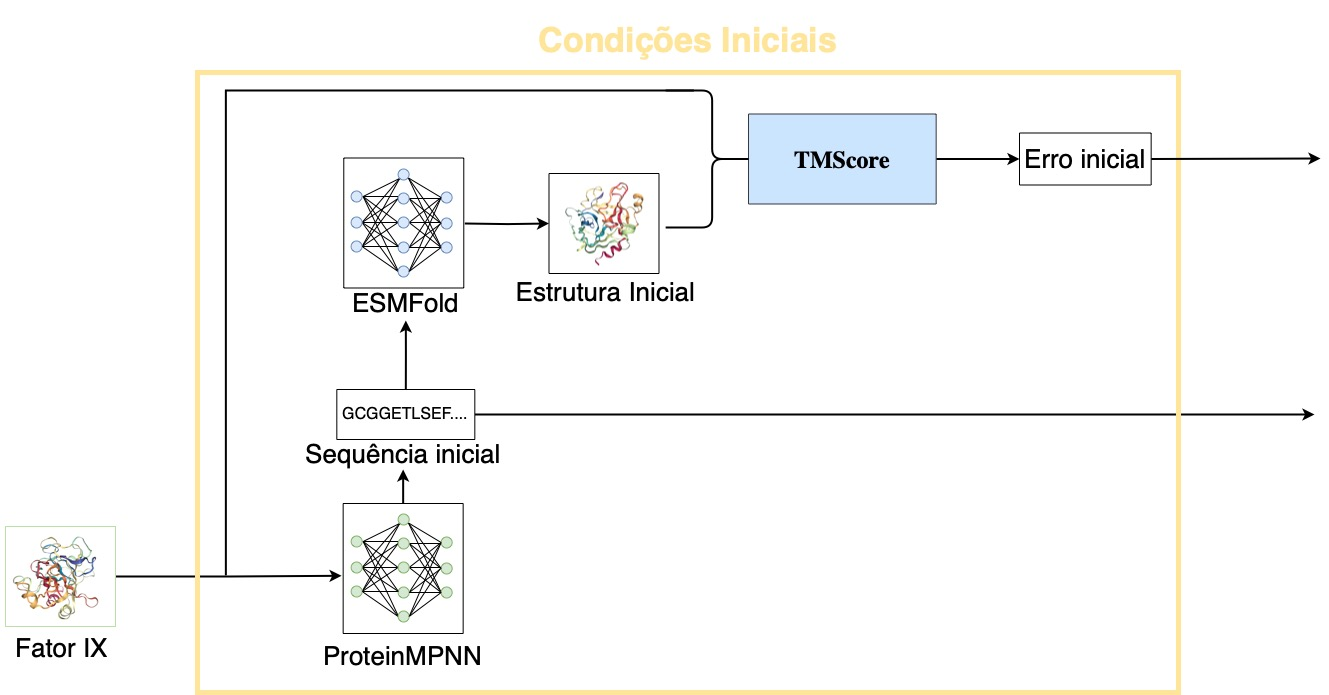
\includegraphics[width=.8\textwidth]{figuras/metodologia-Initial_cond.jpg}
  \caption{Obtenção das condições iniciais}
  \label{fig:cond_iniciais}
\end{figure}

\section{Treinamento}
%iterações entre Agente e Ambiente ok
%Agente é PPO ok
%Acao é mutação ok 
%Imagem da mutação ok 
%Ambiente de aprendizado é modelado por um MDP e é definido quem sao os estados, acoes e  recompensas. É tambem definido a função de transição entre estados (step) e função de reset
O módulo de Treinamento foi construído em duas etapas: Estágios I e II, detalhados em \ref{subsection:stage1} e \ref{subsection:stage2} respectivamente.
Para ambos os estágios, o treinamento se dá através de interações entre dois componentes: O Ambiente de aprendizado e o Agente. 

\subsection{Ambiente de aprendizado}
O ambiente de aprendizado é modelado como um MDP e, portanto, é responsável por definir o espaço de ações, o espaço de estados, a função de transição entre estados dado uma ação e a função de recompensa.  

\subsubsection{Espaço de ações}

Definimos uma ação como um vetor bi-dimensional composto pelo índice $p$ de uma posição na sequência e um aminoácido $r$. 
A ação será utilizada para realizar uma mutação na proteína, inserindo o $r$ na posição $p$. 
De modo a incentivar o Agente a explorar diferentes ações, 
definimos, para cada iteração, um conjunto de posições e aminoácidos válidos: $P_{val}$ e $R_{val}$ respectivamente. 
$P_{val}$ é composto por todas as possíveis posições na sequência, com exceção das posições previamente selecionadas dentro do mesmo episódio. 
Definimos $R_{val}$ sendo igual aos 20 possíveis aminoácidos, com exceção dos aminoácidos que foram selecionados mais de 7 vezes no mesmo episódio. 
Desta forma, o espaço de ações, para cada iteração $i$, é definido por:

\begin{equation}
A_{i} = \left\{(p, r) | p \in P_{val_{i}} , r \in R_{val_{i}} \right\}
\end{equation}
  

\subsubsection{Espaço de estados}
Definimos o espaço de estados como o conjunto de todas as possíveis sequências de $n$ aminoácidos, onde $n$ é o tamanho da sequência inicial:

\begin{equation}
S = \left\{(r_{1}, r_{2}, r_{3}, ..., r_{n}) | r_{i} \in R_{encoded} \forall i \in [1,n] \right\}
\end{equation}

Onde $R_{encoded}$ é o conjunto dos 20 possíveis aminoácidos, 
cada um representado por um vetor codificado pelo \textit{Encoder}. 
O \textit{Encoder} consiste em um dicionário que mapeia cada aminoácido para 
uma representação vetorial que conserva as distâncias entre cada par de aminoácidos estabelecidas por \cite{aminodist}.
Este mapeamento foi construído através de um MDS utilizando 21 dimensões. 

\begin{figure}[H]
  \centering
  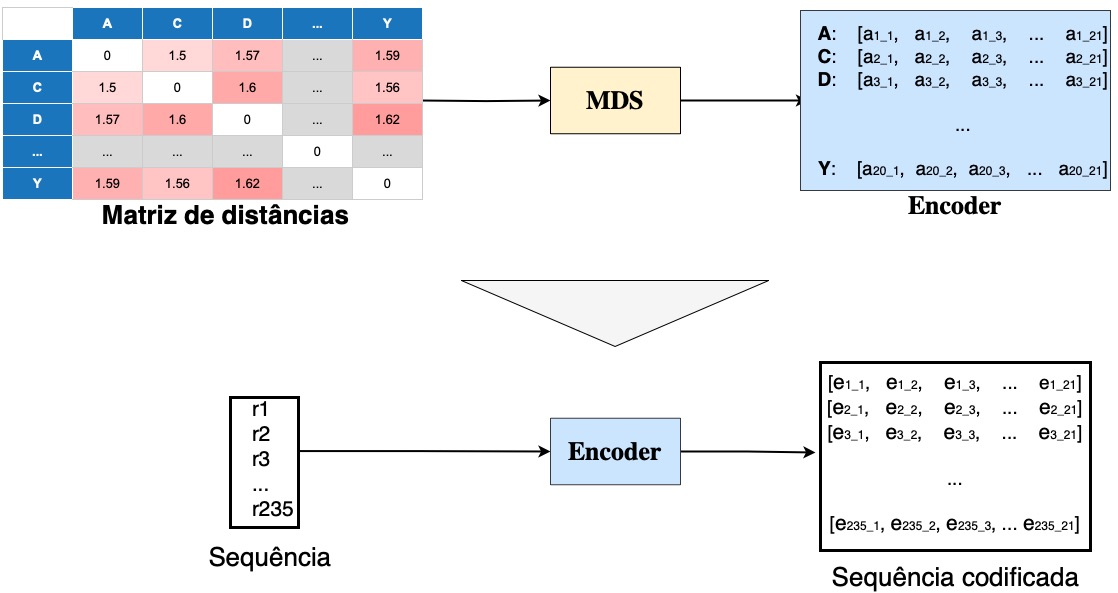
\includegraphics[width=.8\textwidth]{figuras/metodologia-encoder.jpg}
  \caption{Construção e uso do \textit{Encoder}. }
  \label{fig:encoder}
\end{figure}

Para escolher a quantidade de dimensões a se utilizar no MDS, definimos o ponto a partir do qual a curva entre \textit{Stress} e dimensionalidade 
tende a se aproximar assintóticamente do eixo x do plano cartesiano. Este ponto, conforme a figura \ref{fig:best_dim}, é o que possui 21 dimensões. 

\begin{figure}[H]
  \centering
  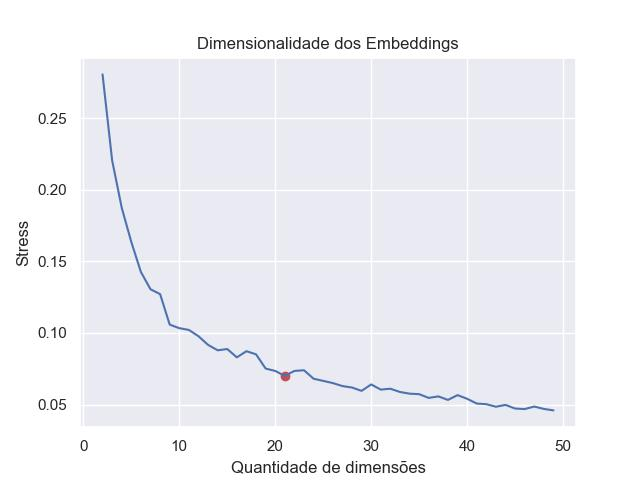
\includegraphics[width=.8\textwidth]{figuras/best_dim.jpg}
  \caption{Escolha da dimensionalidade dos Embeddings}
  \label{fig:best_dim}
\end{figure}



\subsubsection{Função de transição de estados}
A função de transição de estados é caracterizada pela geração de uma nova sequência, 
resultante da mutação definida pelo Agente. 
Em outras palavras, é uma função que tem como entrada uma ação e o estado atual e como saída o estado resultante da transição. 

\begin{figure}[H]
  \centering
  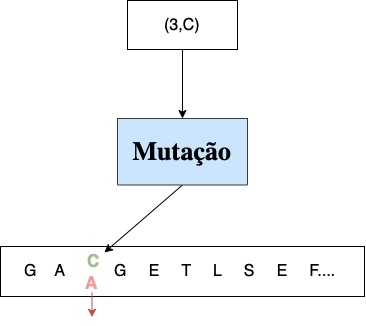
\includegraphics[width=.5\textwidth]{figuras/metodologia-Mutation.jpg}
  \caption{Exemplo de mutação. O aminoácido A na posição 3 está sendo substituído pelo o aminoácido C}
  \label{fig:mutacao}
\end{figure}

\subsubsection{Função de recompensa}
Já a função de recompensa calcula a qualidade da ação selecionada pelo Agente. 
Nas seções \ref{subsection:stage1} e \ref{subsection:stage2} especificamos a função de recompensa de cada estágio de treinamento.


\subsection{Agente}
\label{subsection:Agente}
O Agente é modelado por uma rede neural, batizada de \textit{GenSeq}, cujos parâmetros são otimizados através da técnica \textit{Proximal Policy Optimization} (PPO), 
sendo responsável por decidir qual a melhor mutação a se fazer, dada a sequência de entrada. Em outras palavras, o Agente deve escolher,
dentro do espaço de ações, a ação que maximiza a recompensa acumulada.
Os hiperparâmetros utilizados no Agente são apresentados na tabela a seguir. 

\begin{table}[H]
\centering
\vspace{0.5cm}
\begin{tabular}{r|lr}
Hiperparâmetro & Valor \\ 
\hline                               
Número de camadas escodidas & 2 \\
Número de neurônios por camada escondida & 64 \\
Função de ativação & tangente hiperbólica \\
Otimizador & Adam \\
Taxa de aprendizagem & 3e-4 \\
Número de épocas & 10 \\
Fator de desconto ($\gamma$) & 0.99 \\
\end{tabular}
\caption{Hiperparâmetros do PPO}
\end{table}

Após ser processada pelo \textit{Encoder}, a sequência passa pela camada de entrada do \textit{GenSeq} e 
segue para duas camadas escondidas de 64 dimensões cada. 
A camada de saída, por sua vez, possui 255 unidades, organizadas em duas partes:

\begin{enumerate}
  \item As primeiras 235 unidades da camadas estão associadas ao primeiro atributo da ação: A posição $p$ da sequência de entrada
  que deve sofrer mutação. A posição predita pelo Agente corresponde ao índice da unidade de saída com maior valor entre as 235 primeiras. 
  \item Já as 20 últimas unidades de saída estão associadas ao segundo atributo da ação: O índice do aminoácido $r$ que o Agente sugere inserir na posição $p$.
  Este valor corresponde ao índice da unidade de saída com maior valor entre as 20 últimas unidades, subtraído de 235.
\end{enumerate}

Por exemplo, suponha que, entre as 235 primeiras unidades, a de maior valor é a terceira, e que, entre as 20 útltimas, o maior valor esteja na unidade 240. 
Nesse caso, a ação sugerida pelo Agente é fazer uma mutação na posição 3, inserindo o aminoácido de índice 5.

\begin{figure}[H]
  \centering
  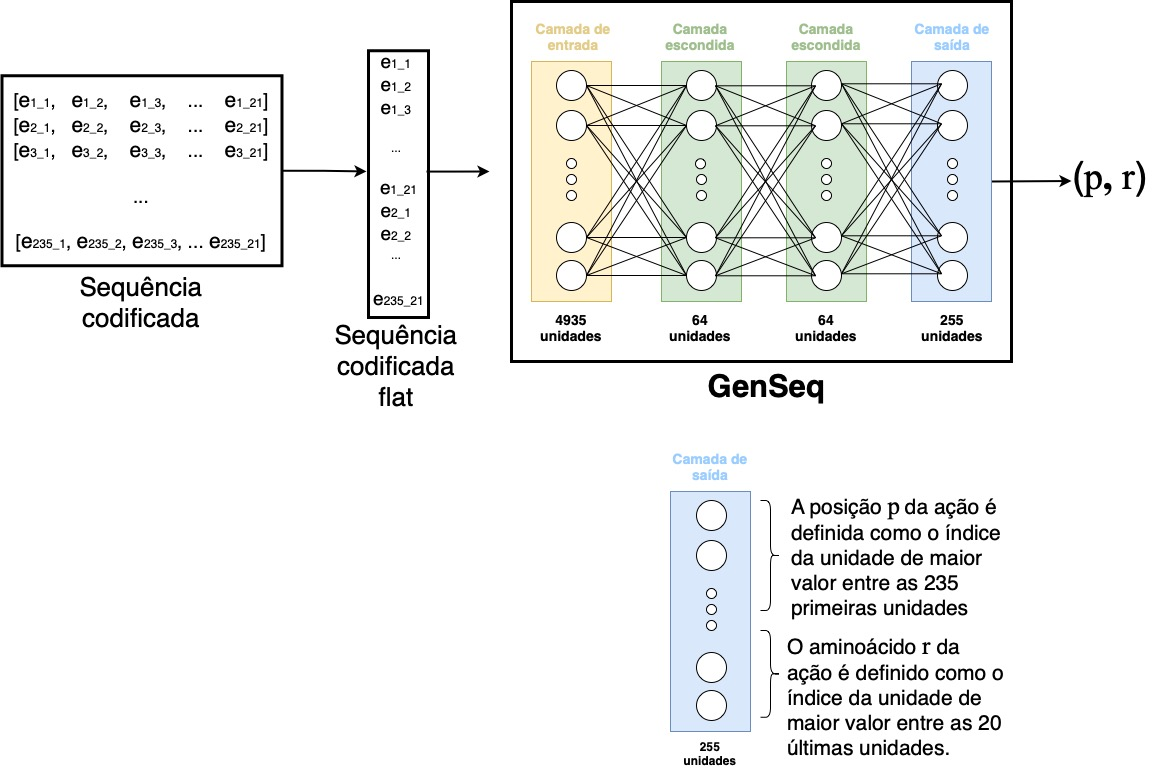
\includegraphics[width=.8\textwidth]{figuras/metodologia-NN_arch_actor.jpg}
  \caption{Arquitetura da rede neural do Agente (\textit{GenSeq})}
  \label{fig:actor_arch}
\end{figure}


\subsection{Treinamento - Estágio I}
\label{subsection:stage1}
%Definição de episodio 
%Vitoria ou derrota no episodio
%Numero de steps total e por episodio

Tendo em vista o vasto número de ações possíveis, 
desenvolvemos o Estágio I de treinamento com o objetivo de estimular o Agente a encontrar um subespaço menor de ações para atuar.
Para isso, atribuímos recompensas negativas (ou penalizações) para ações em posições da sequência cujo o \textit{Conservation Score} é alto,
bem como penalizamos ações onde o aminoácido substituído é muito diferente do que fora inserido. 
Neste sentido, definimos a seguinte função de recompensa:

\begin{equation}
    R_{I} = -(CS(p) + AminoDist(r, r_{prev}))
\end{equation}

\noindent
Onde $p$ e $r$ são a posição e o aminoácido selecionados pelo Agente, respectivamente. O $r_{prev}$ é o aminoácido que estava na posição $p$ antes da mutação. 
$CS(p)$ é o \textit{Conservation Score} normalizado da posição $p$ e $AminoDist(r, r_{prev})$ é a medida de similariedade entre os aminoácidos $r$ e $r_{prev}$. 

Neste sentido, o primeiro estágio de treinamento consiste do seguinte procedimento:

\begin{enumerate}
  \item Os pesos do \textit{GenSeq} são inicializados aleatóriamente.
  \item Inicializa o episódio com a sequência inicial e com $P_{val}$ sendo todas as posições da sequência e $R_{val}$ sendo todos os 20 aminoácidos 
  \item A sequência atual é codificada pelo \textit{Encoder}.
  \item \textit{GenSeq} estima a melhor ação $(p,r)$ baseado na sequência codificada. 
  \item A sequência atual é modificada ao inserir $r$ na posição $p$.
  \item Baseado em $(p,r)$ e $r_{prev}$, é calculado $R_{I}$.
  \item $p$ é removido de $P_{val}$ e se a quantidade de vezes que $r$ foi utilizado pelo \textit{GenSeq} é maior ou igual a 7, então $r$ é retirado de $R_{val}$.
  \item Se a iteração atual é igual ao tamanho do \textit{batch}, então \textit{GenSeq} atualiza seus pesos baseado nos valores obtidos de $R_{I}$ utilizando o \textit{PPO}
  \item Se foi atingido o máximo de mutações por episódio, então o episódio é finalziado.
  \item Repete a partir do item 2 até atingir o número máximo de iterações. 
\end{enumerate}


\begin{figure}[H]
  \centering
  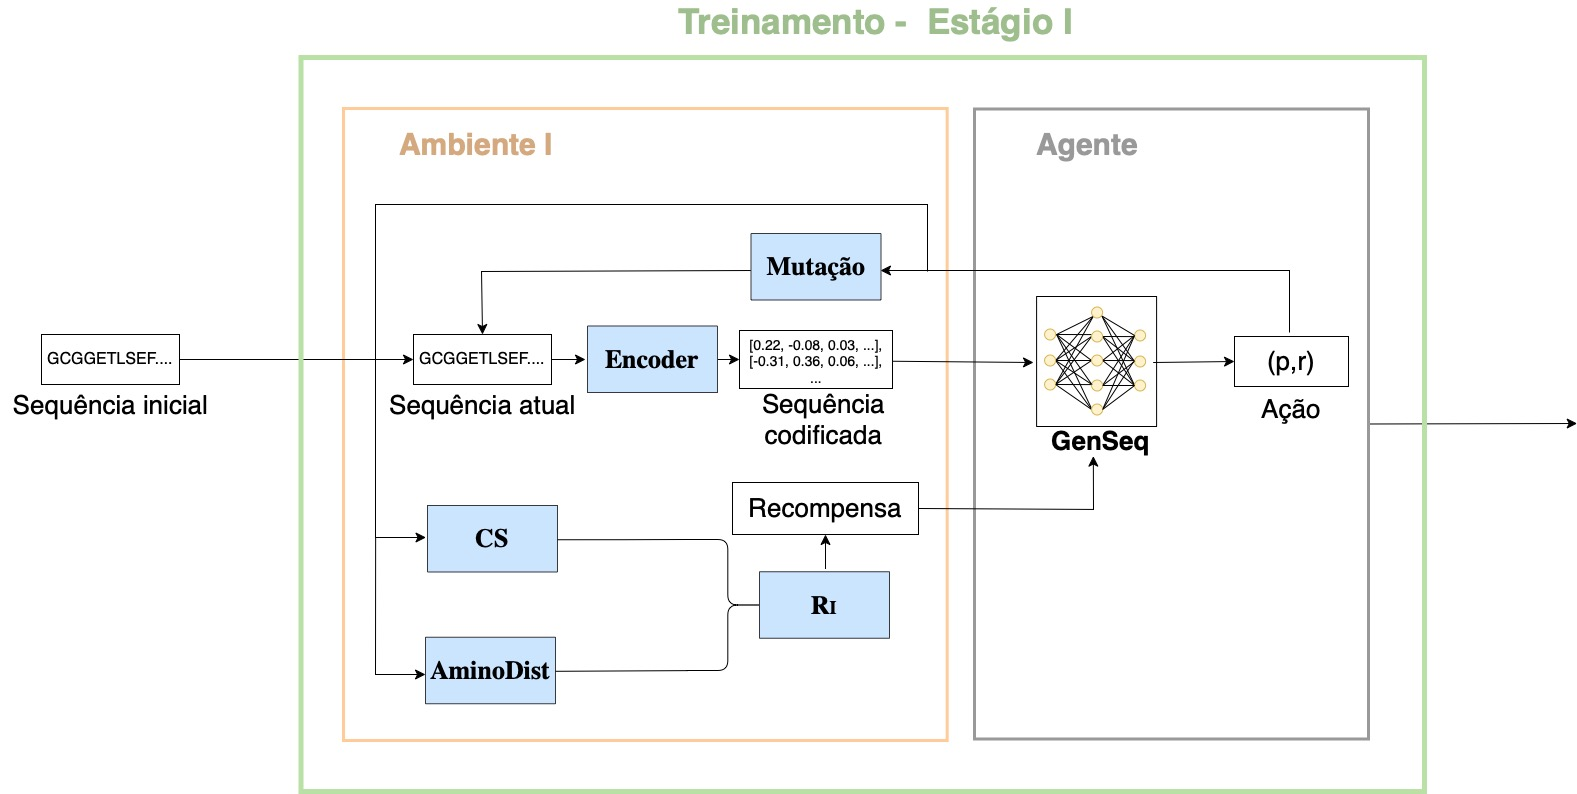
\includegraphics[width=.9\textwidth]{figuras/metodologia-Pre-Training.jpg}
  \caption{Primeiro estágio de treinamento}
\end{figure}

Neste estágio, o Agente foi treinado com um total de 2 milhões de iterações, podendo executar até 100 mutações por episódio.
\begin{table}[H]
  \centering
  \vspace{0.5cm}
  \begin{tabular}{r|lr}
  Parâmetro & Valor \\ 
  \hline                               % para uma linha horizontal
  Número máximo de mutações por episódio & 100 \\
  Número de iterações & 2.000.000 \\
  Tamanho do \textit{batch} & 200 \\
  \end{tabular}
  \caption{Parâmetros preliminares}
  \end{table}

  Após finalizado o primeiro estágio, comparamos o desempenho do Agente com o desempenho de uma política que define ações aleatoriamente, onde observamos
  que a mediana da distribuição de recompensas do Agente é consideravelmente superior ao do Agente aleatório. 

  \begin{figure}[H]
    \centering
    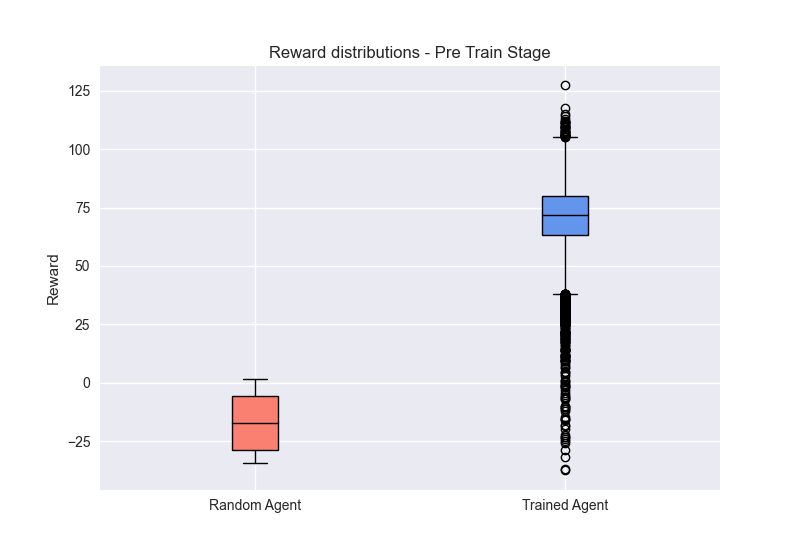
\includegraphics[width=.8\linewidth]{figuras/plot_box_pre_train_reward.jpg}  
    \caption{Comparação do Agente pré treinado com um Agente aleatório}
    \label{fig:box-pre-train}
  \end{figure}

Observa-se que o Agente atingiu um platô de recompensas no ambiente I com cerca de 2500 episódios, como ilustrado em 
\ref{fig:rew_per_ep_pretrain}.

  \begin{figure}[H]
    \centering
    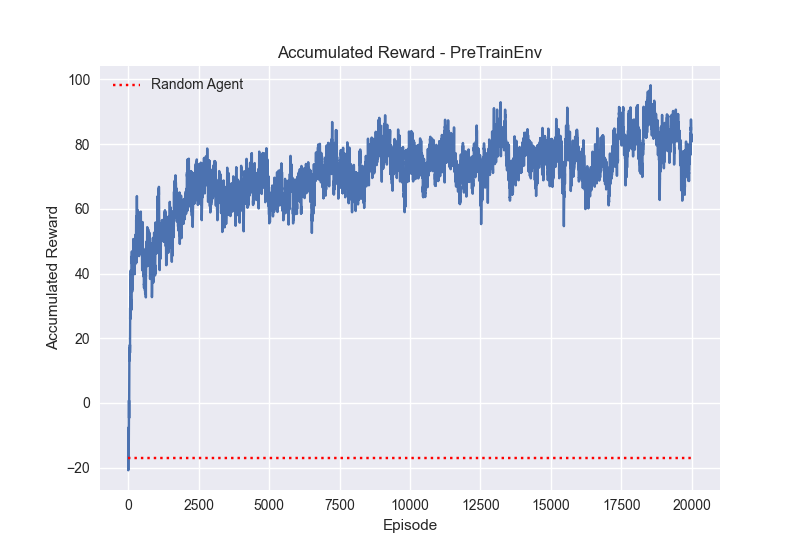
\includegraphics[width=.8\linewidth]{figuras/plot_pre_train_reward.jpg}    
    \caption{Média móvel das recompensas por episódio - treino}
    \label{fig:rew_per_ep_pretrain}
  \end{figure}


\subsection{Treinamento - Estágio II}
\label{subsection:stage2}
%Função do reward
%Numero de steps total e por episodio
%Vitoria ou derrota no episodio
O objetivo do segundo estágio de treinamento é fazer com que o agente pré treinado aprenda a escolher ações que maximizem o \textit{TM-Score} entre a estrutura gerada e a alvo, 
i.e, minimizem o erro $1-TMScore$.
Para isto, definimos a função de recompensa como a soma de 3 termos: 

\begin{equation}
    R_{II} = -aEr_{i} + b(Er_{0} - Er_{i}) + c(Er_{i-1} - Er_{i})
\end{equation}

\noindent
Onde $Er_{i}$ e $Er_{i-1}$ são os erros da iteração i e i-1 respectivamente, e $a, b$ e $c$ são constantes. 
O primeiro termo, $-aEr_{i}$, é a penalização pelo erro atual.
O segundo determina uma penalização se o erro atual for maior que o inicial e uma recompensa caso contrário.
Análogamente, o terceiro termo penaliza se o erro atual for maior que o anterior e recompensa se for menor.
Como o objetivo principal é encontrar sequências com erro menores que o inicial, atribuímos um peso maior ao segundo termo, i.e, $b>a$ e $b>c$.
Além disso, consideramos $c>a$ para valorizar reduções do erro ao longo do episódio.  

Introduzimos também o conceito de vitória e derrota a cada episódio. 
Consideramos vitória caso o erro final seja menor que o inicial e derrota caso contrário. 
De modo a valorizar a vitória e penalizar a derrota, ao final de cada episódio é adicionado uma recompensa adicional dada por $2500(Er_{0} - Er_{f})$, 
onde $Er_{f}$ é o erro final, i.e, da última iteração do episódio. Cada episódio é finalizado ao se atingir um número máximo de iterações, ou um limiar de erro. 
Foi definido um limite superior para o erro de modo a evitar que o Agente atinja erros muito grandes em um mesmo episódio,
e um limite inferior para valorizar episódios em que o Agente foi capaz de encontrar "atalhos", i.e, conseguiu reduzir o erro considerávelmente em poucas iterações.

Neste sentido, o segundo estágio de treinamento consiste do seguinte procedimento:

\begin{enumerate}
  \item Inicializa o episódio com a sequência e o erro inicial; $P_{val}$ sendo todas as posições da sequência; $R_{val}$ sendo todos os 20 aminoácidos.
  \item A sequência atual é codificada pelo \textit{Encoder}.
  \item \textit{GenSeq} estima a melhor ação $(p,r)$ baseado na sequência codificada. 
  \item A sequência atual é modificada ao inserir $r$ na posição $p$.
  \item É predito a estrutura da sequência atual utilizando o \textit{ESMFold}
  \item Baseado no \textit{TMScore} entre a estrutura do Fator IX e da estrutura atual, no erro inicial e no erro da iteração anterior, é calculado $R_{II}$.
  \item $p$ é removido de $P_{val}$ e, se a quantidade de vezes que $r$ foi utilizado pelo \textit{GenSeq} é maior ou igual a 7, então $r$ é retirado de $R_{val}$.
  \item Se a iteração atual é igual ao tamanho do \textit{batch}, então \textit{GenSeq} atualiza seus pesos baseado nos valores obtidos por $R_{II}$ utilizando o \textit{PPO}
  \item Se foi atingido o máximo de mutações por episódio, ou um limiar de erro, então o episódio é finalziado e é atribuído a recompensa adicional igual a $2500(Er_{0} - Er_{f})$.
  \item Repete a partir do item 1 até atingir o número máximo de iterações. 
\end{enumerate}

\begin{figure}[H]
  \centering
  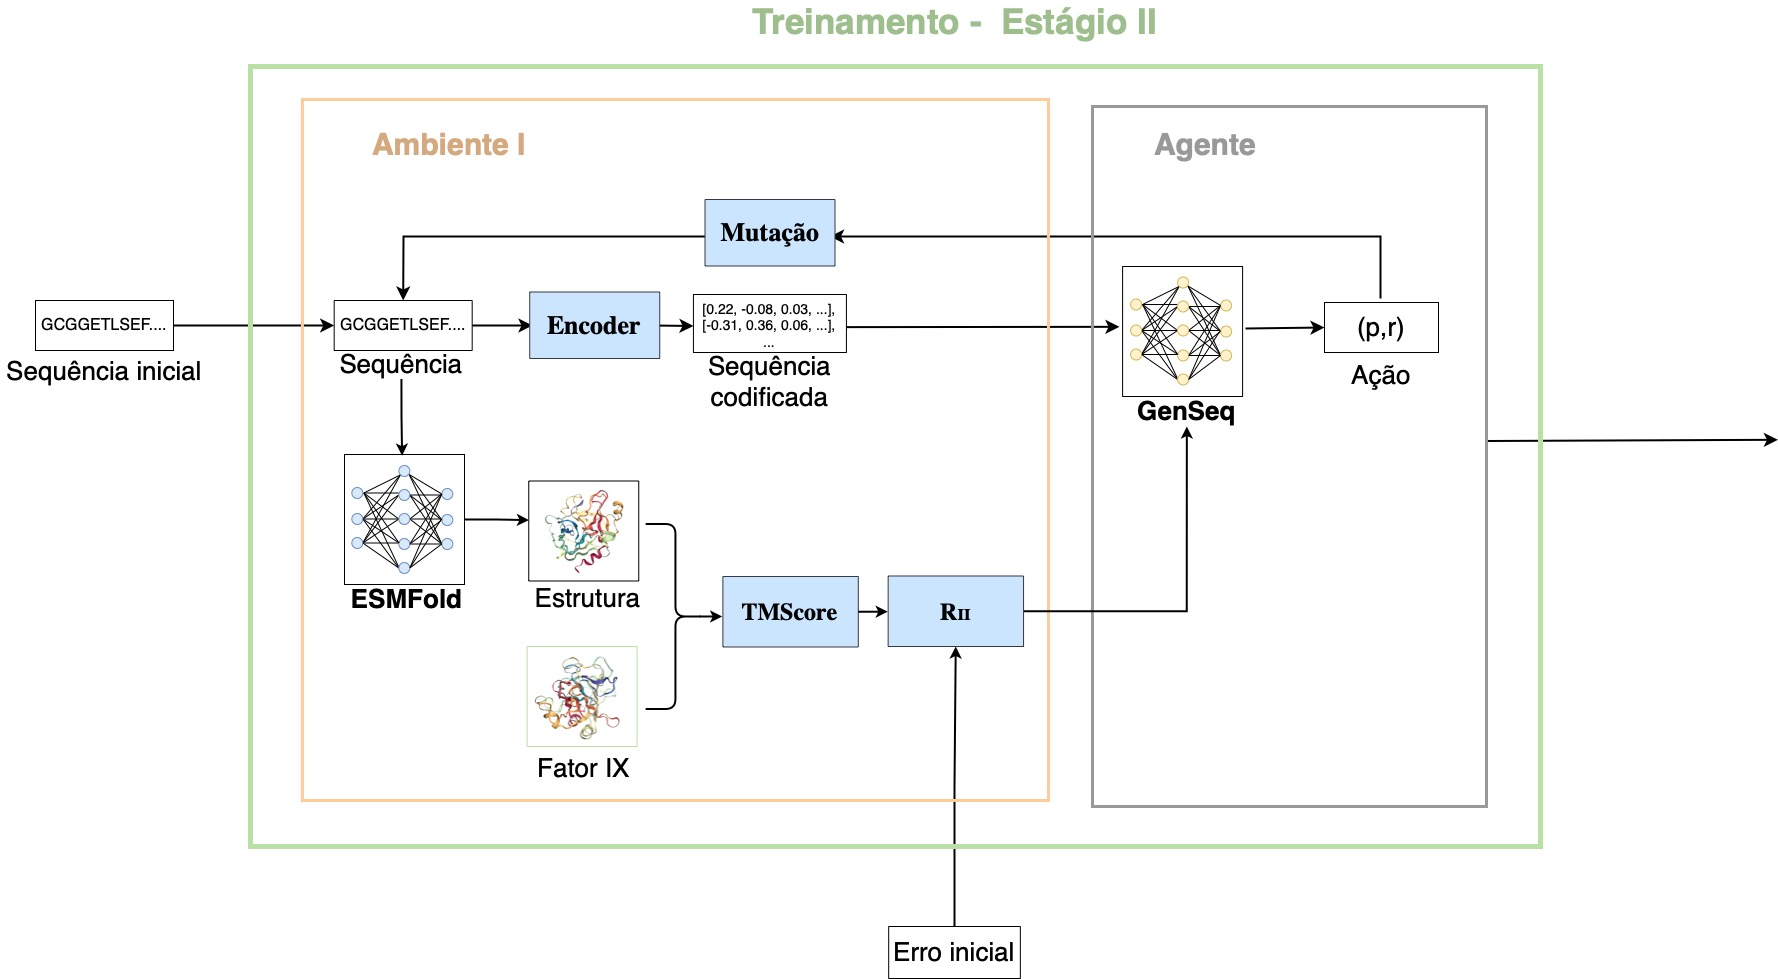
\includegraphics[width=.8\textwidth]{figuras/metodologia-Training.jpg}
  \caption{Segundo estágio - Treino}
\end{figure}

Neste estágio, o Agente foi treinado com um total de 60 mil de iterações, podendo executar até 45 mutações por episódio. 

\begin{table}[H]
  \centering
  \vspace{0.5cm}
  \begin{tabular}{r|lr}
  Parâmetro & Valor \\ 
  \hline                               % para uma linha horizontal
  Número máximo de mutações por episódio & 45 \\
  Erro mínimo no episódio & 0.05 \\
  Erro máximo no episódio & 0.083 \\
  Número de iterações & 60.000 \\
  a & 12 \\
  b & 200 \\
  c & 50 \\
  \end{tabular}
  \caption{Parâmetros preliminares}
  \end{table}

  Assim como no pré treino, a distribuição das recompensas do Agente ao longo do treinamento é 
  bem superior às recompensas de um Agente aleatório.  
  \begin{figure}[H]
    \centering
    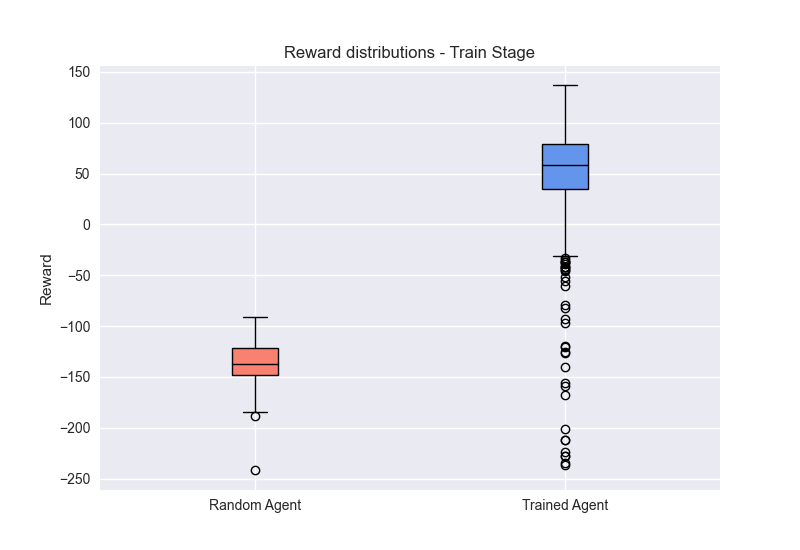
\includegraphics[width=.9\linewidth]{figuras/plot_box_train_reward.jpg}  
    \caption{Comparação do Agente treinado com um Agente aleatório}
    \label{fig:box-train}
  \end{figure}

  Repare que, devido ao pré treino, as recompensas médias do Agente são consideravelmente superiores
  à recompensa média do Agente aleatório desde os primeiros episódios. 
  \begin{figure}[H]
    \centering
    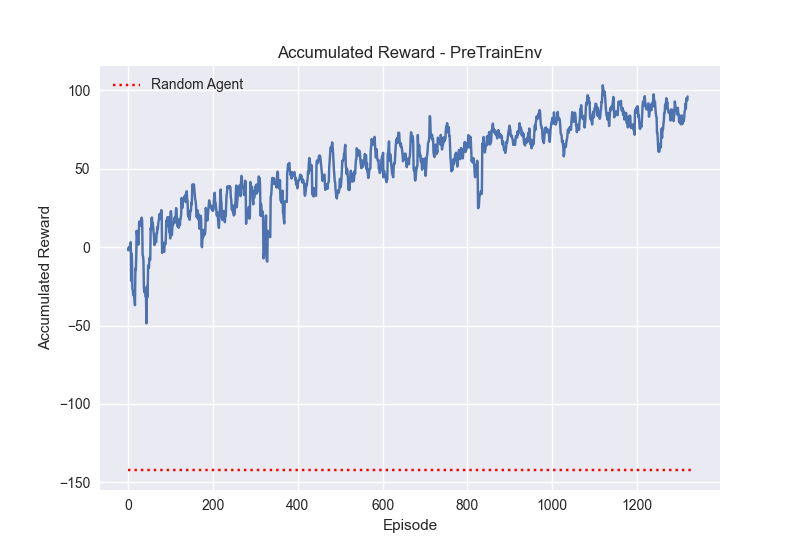
\includegraphics[width=.8\linewidth]{figuras/plot_train_reward.jpg}    
    \caption{Média móvel das recompensas por episódio - treino}
    \label{fig:rew_per_ep_train}
  \end{figure}
  

\section{Geração de sequências}
Por fim, o módulo de Geração de Sequências utiliza o agente treinado para gerar novas sequências que sejam capazes de mimetizar a estrutura alvo melhor do que a sequência inicial, em termos de \textit{TM-Score}.  
\begin{figure}[H]
  \centering
  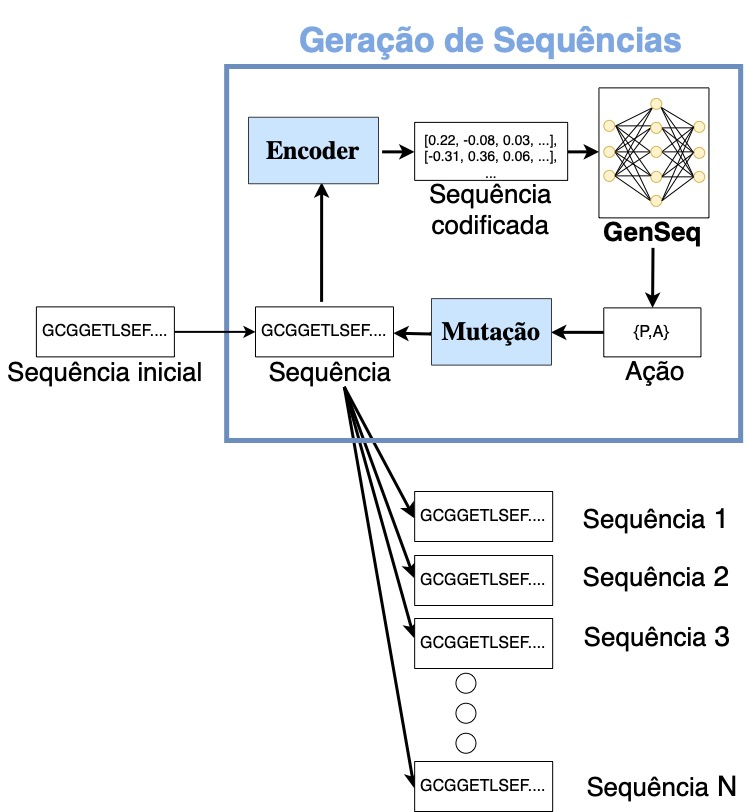
\includegraphics[width=.8\textwidth]{figuras/metodologia-Generating.jpg}
  \caption{Gerando sequência otimizada}
  \label{fig:geradorseq}
\end{figure}

\chapter{Resultados}

Com o Agente treinado, é possível gerar novas sequências seguindo a arquitetura 
ilustrada na figura \ref{fig:geradorseq}. 
O Agente gerou mais de 200 proteínas diferentes a partir de mutações na sequência inicial. 
De modo a identificar cada proteína, 
vamos considerar a ordem com que foi gerada como seu respectivo ID.
Filtramos as proteínas geradas baseado em um limiar de 92\% de TMScore.
Com isso, selecionamos as 63 primeiras sequências.  

\begin{figure}[H]
    \centering
    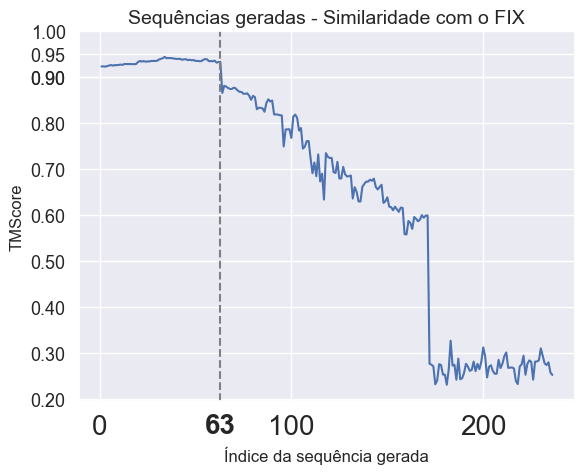
\includegraphics[width=.6\linewidth]{figuras/plot_tmscore_decreasing.png}    
    \caption{Variação da similaridade entre as sequências geradas e o FIX }
    \label{fig:tmscore_decreasing}
  \end{figure}


A proteína gerada que é estruturalmente mais similar ao FIXa é a de ID 34,
tendo TMScore igual a 94.48\% e RMSD de 1.485 angstroms. 

\begin{figure}[H]
    \centering
    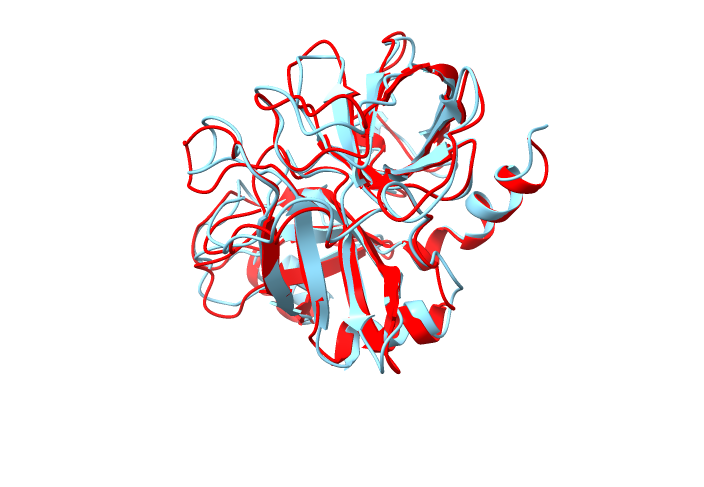
\includegraphics[width=.6\linewidth]{figuras/FIXvsID34.png}    
    \caption{Alinhamento entre FIX (em azul) e a proteína ID 34 (em vermelho)}
    \label{fig:FIX_vs_ID34}
\end{figure}

Os resultados obtidos demonstram que o agente \textit{GenSeq} foi capaz de gerar sequências de aminoácidos que
estão associadas a estruturas com elevado grau de similaridade ao FIX nativo.
Considerando que o valor de \textit{TMScore} superior a 0.5 já indica similaridade estrutural significativa \cite{05TMScore},
os valores obtidos sugerem que as proteínas geradas mantêm a conformação global e o dobramento necessários para funcionalidade.

É interessante notar que, apesar da forte semelhança estrutural entre as proteínas,
em termos de IS (Idêntidade de Sequência)
são sequências muito diferentes, tendo em média apenas 30\% de similaridade. 
  
\begin{table}[htbp]
    \centering
    \begin{tabular}{c|cccc}
        \hline
        \textbf{ID} & \textbf{TM-Score} & \textbf{RMSD} & \textbf{IS - seq. original} \\
        \hline
         20 & 93.33\% & 1.75 Å & 30.64\% \\
         30 & 93.62\% & 1.68 Å & 30.21\% \\
         34 & 94.48\% & 1.48 Å & 29.79\% \\
         63 & 93.36\% & 1.72 Å & 26.81\% \\
        \hline
    \end{tabular}
    \caption{Generated proteins}
    \label{tab:tabela_exemplo}
\end{table}



\section{Resposta imunológica}
\label{section:imuno_resultados}
Para mensurar a propensão das proteínas geradas provocarem uma resposta imunológica no organismo, 
calculamos o \textit{binding affinity} de cada proteína com os epítopos de quatro grupos diferentes 
de alelos apresentados na tabela \ref{tab:alelo_grupos}


    \begin{table}[]
        \begin{tabular}{|c|c|}
        \hline
        \rowcolor[HTML]{C0C0C0} 
        {\color[HTML]{343434} Grupo} & {\color[HTML]{343434} Frequência em seres humanos} \\ \hline
        DP                                                                         & 25\%                                                                           \\ \hline
        DQ                                                                         & 20\%                                                                           \\ \hline
        DRB1                                                                       & 5\%                                                                            \\ \hline
        DRB3\_4\_5                                                                 & 21\%                                                                           \\ \hline
        \end{tabular}
        \caption{Grupos de alelos considerados e a frequência com que ocorrem em seres humanos.}
        \label{tab:alelo_grupos}
        \end{table}


Para esta análise, levamos em consideração apenas epítopos associados a valores de \textit{binding affinity} 
menores que 500nm, indicando ligação forte. 
Nas figuras a seguir é possível visualizar a quantidade, \textit{binding affinity} e frequência de ocorrência 
dos epítopos por cada grupo de alelo. Ao se comparar o resultado do FIX e da proteína de ID 63,
é possível notar uma redução significativa da quantidade de epítopos com ligação forte, influênciado principalmente 
pelo resultado do grupo DRB1. 

\begin{figure}%
    \centering
    \subfloat[\centering Resposta imune FIX ]{{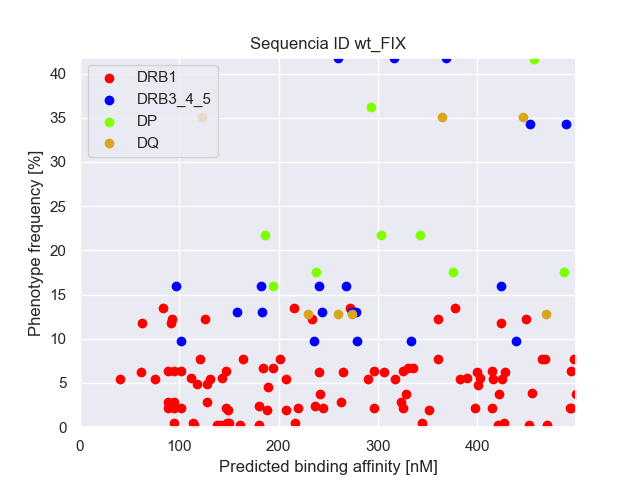
\includegraphics[width=6cm]{figuras/plot_immuno_wt_FIX.png} }}%
    \qquad
    \subfloat[\centering Resposta imune ID 63]{{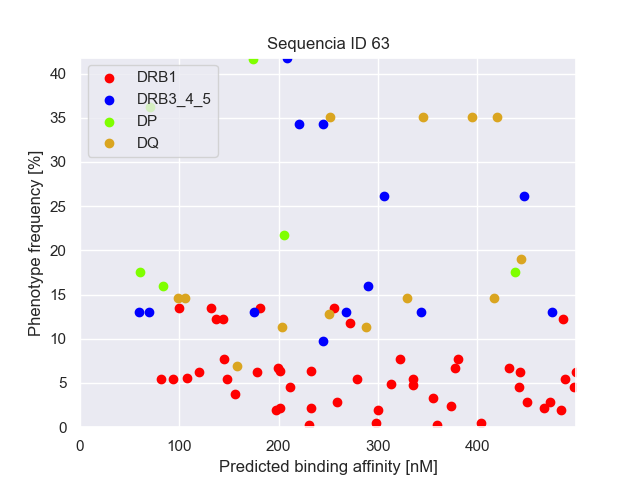
\includegraphics[width=6cm]{figuras/plot_immuno_B_v2_step_63.png} }}%
    %\caption{Comparação entre estruturas}
    %\label{fig:example}%
\end{figure}

A propensão a provocar uma resposta imune não está apenas relacionada a quantidade de epítopos, 
mas também é diretamente proporcional a frequência de ocorrência dos alelos e inversamente proporcional 
ao \textit{binding affinity}. Neste sentido, para mensurar qual proteína induz a uma melhor resposta imune, propomos a 
métrica $IMI$ (Imuno Índice), que consiste na média da razão entre \textit{binding affinity} (${Af}_{i}$) 
e frequência ($Fr_{i}$), 
dividido pela quantidade de epítopos (N):

\begin{equation}
    IMI = \frac{1}{N} \sum_{i=1}^{N} \frac{1}{N} \frac{{Af}_{i}}{Fr_{i}}
\end{equation}

Desta forma, a proteína associada ao maior IMI possui o menor risco de induzir a uma resposta imune.
De modo geral, as 4 últimas sequências geradas possuem um IMI superior ao do FIX: IDs 60, 61, 62 e 63.

\begin{figure}[H]
    \centering
    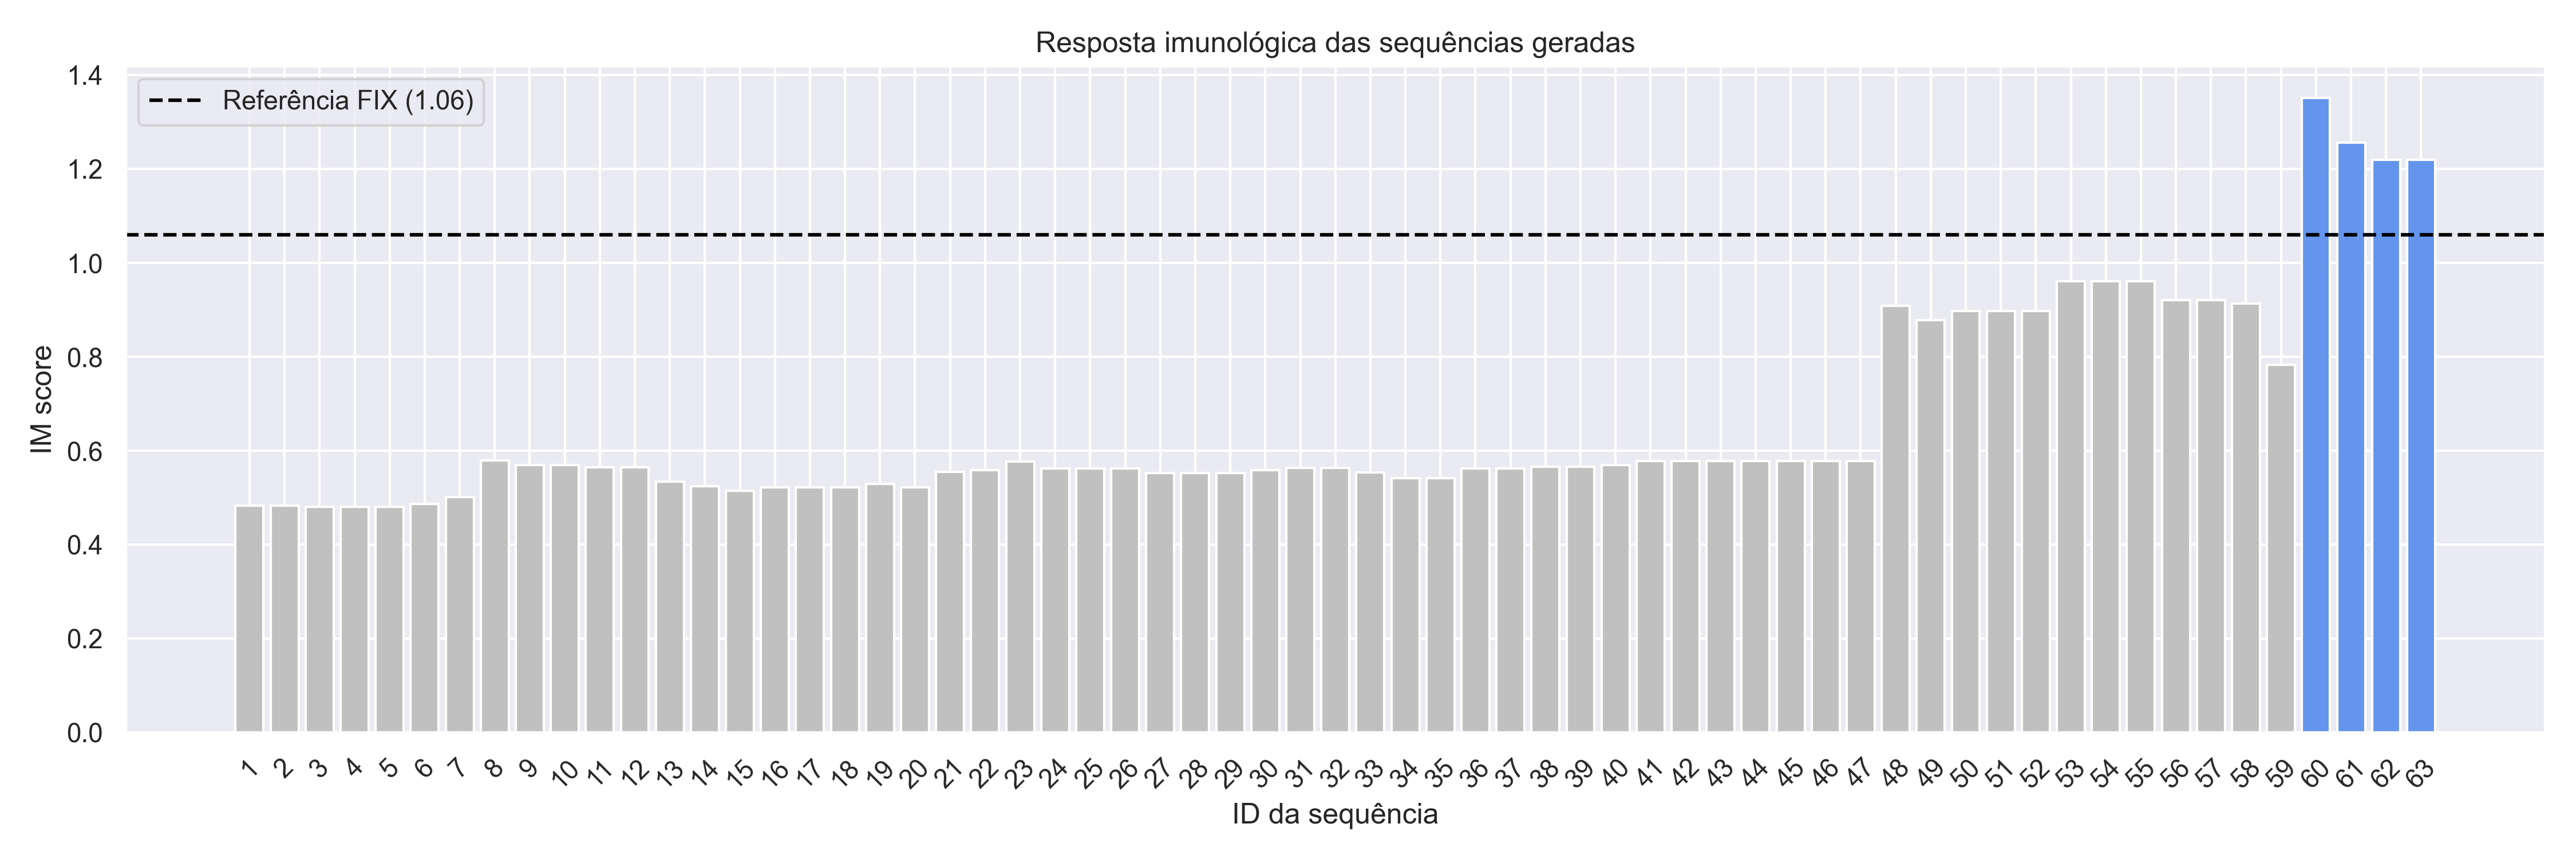
\includegraphics[width=.9\linewidth]{figuras/plot_imuno_IMscore_geral.png}    
    \caption{Comparação do IM entre as proteínas geradas e o FIX}
    \label{fig:immuno_tscore}
\end{figure}

Calculando o IMI para cada grupo de alelo separadamente, observa-se que grande parte das sequências geradas possuem uma resposta 
imune mais favorável que o FIX para os grupos DRB3, DRB4 e DRB5. 
Para o grupo DRB1, as sequências a partir do ID 48 em diante obtiveram IMI superior ao FIX. 
Já para os grupos DQ e DP, nenhuma sequência superou o IMI do FIX. 

\begin{figure}[H]
    \centering
    \begin{minipage}{0.9\textwidth}
        \centering
        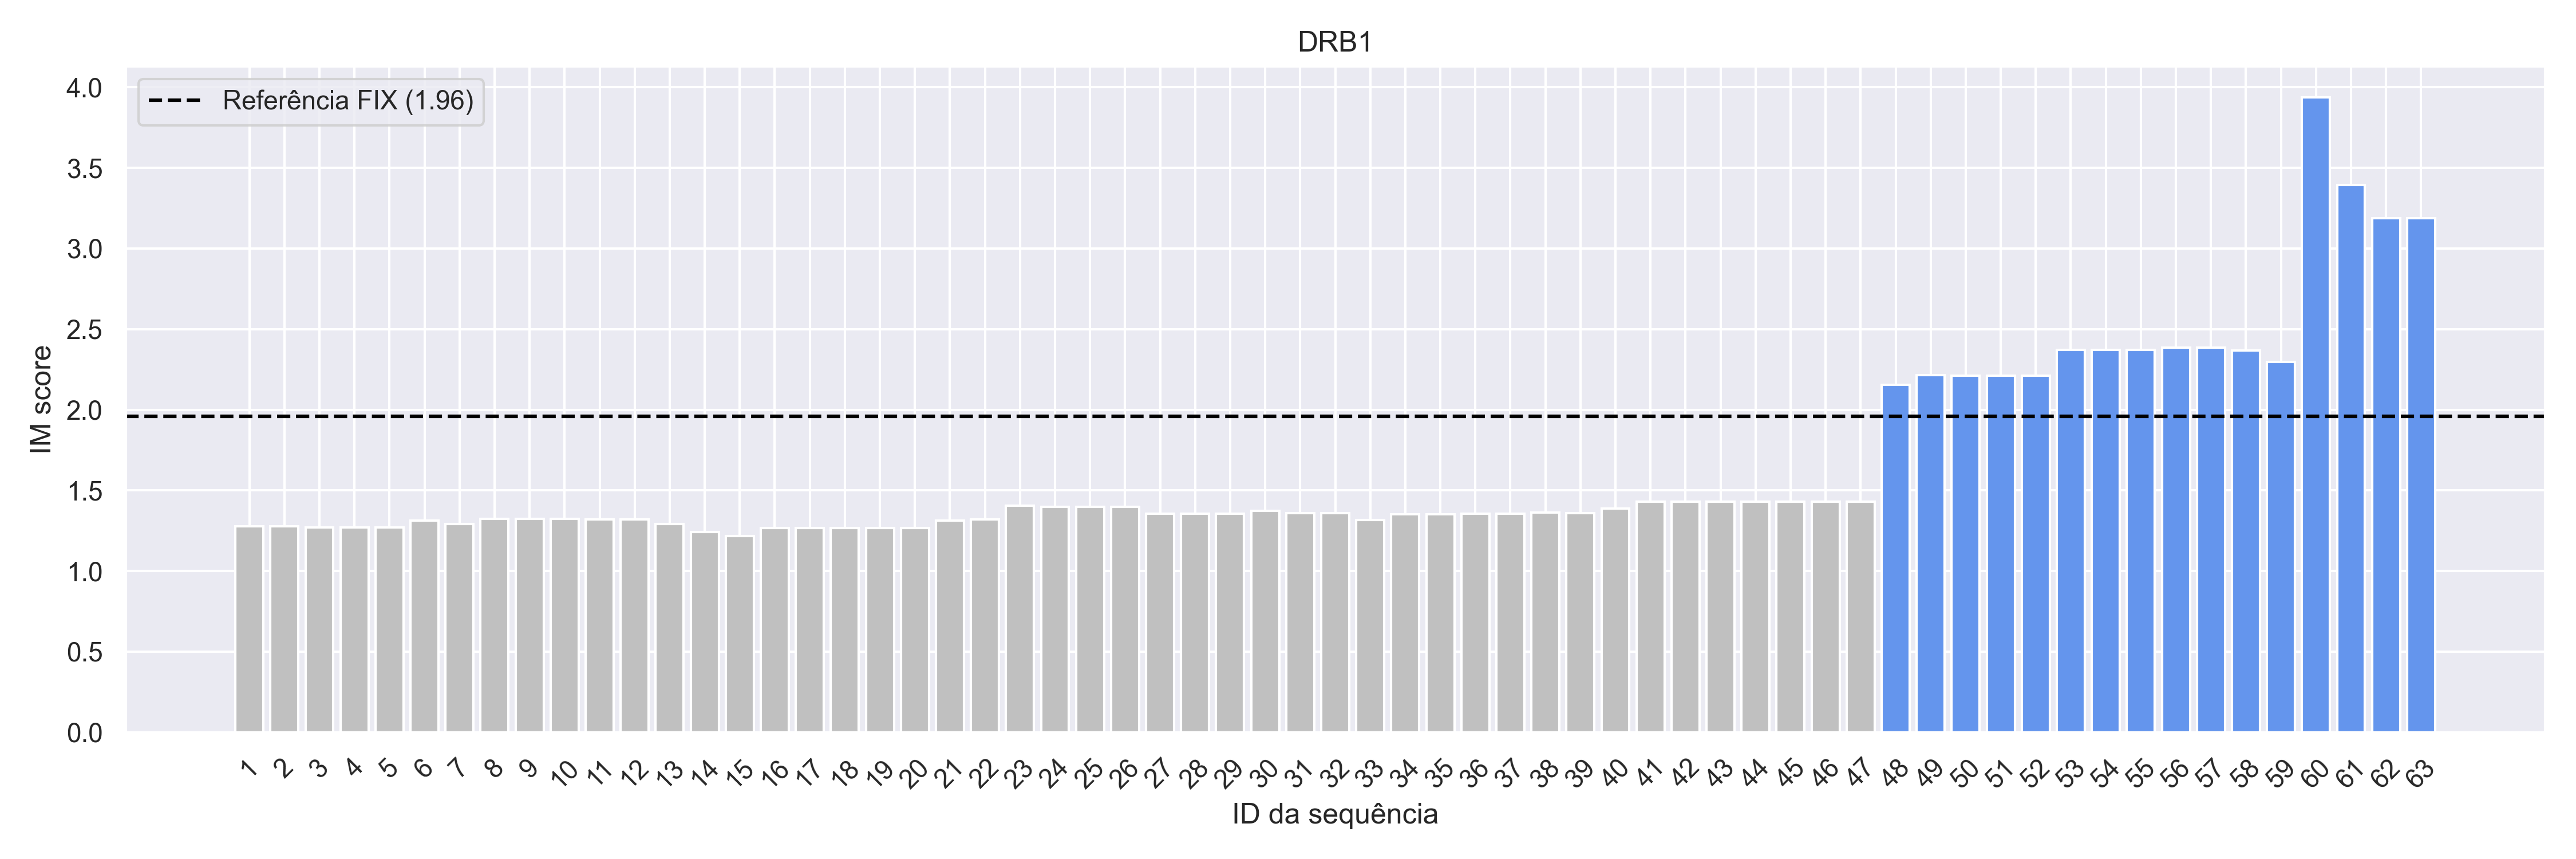
\includegraphics[width=\textwidth]{figuras/plot_imuno_IMscore_DRB1.png}
        %\caption{IM do grupo DRB1}
    \end{minipage} \\[1ex]%
    \begin{minipage}{0.9\textwidth}
        \centering
        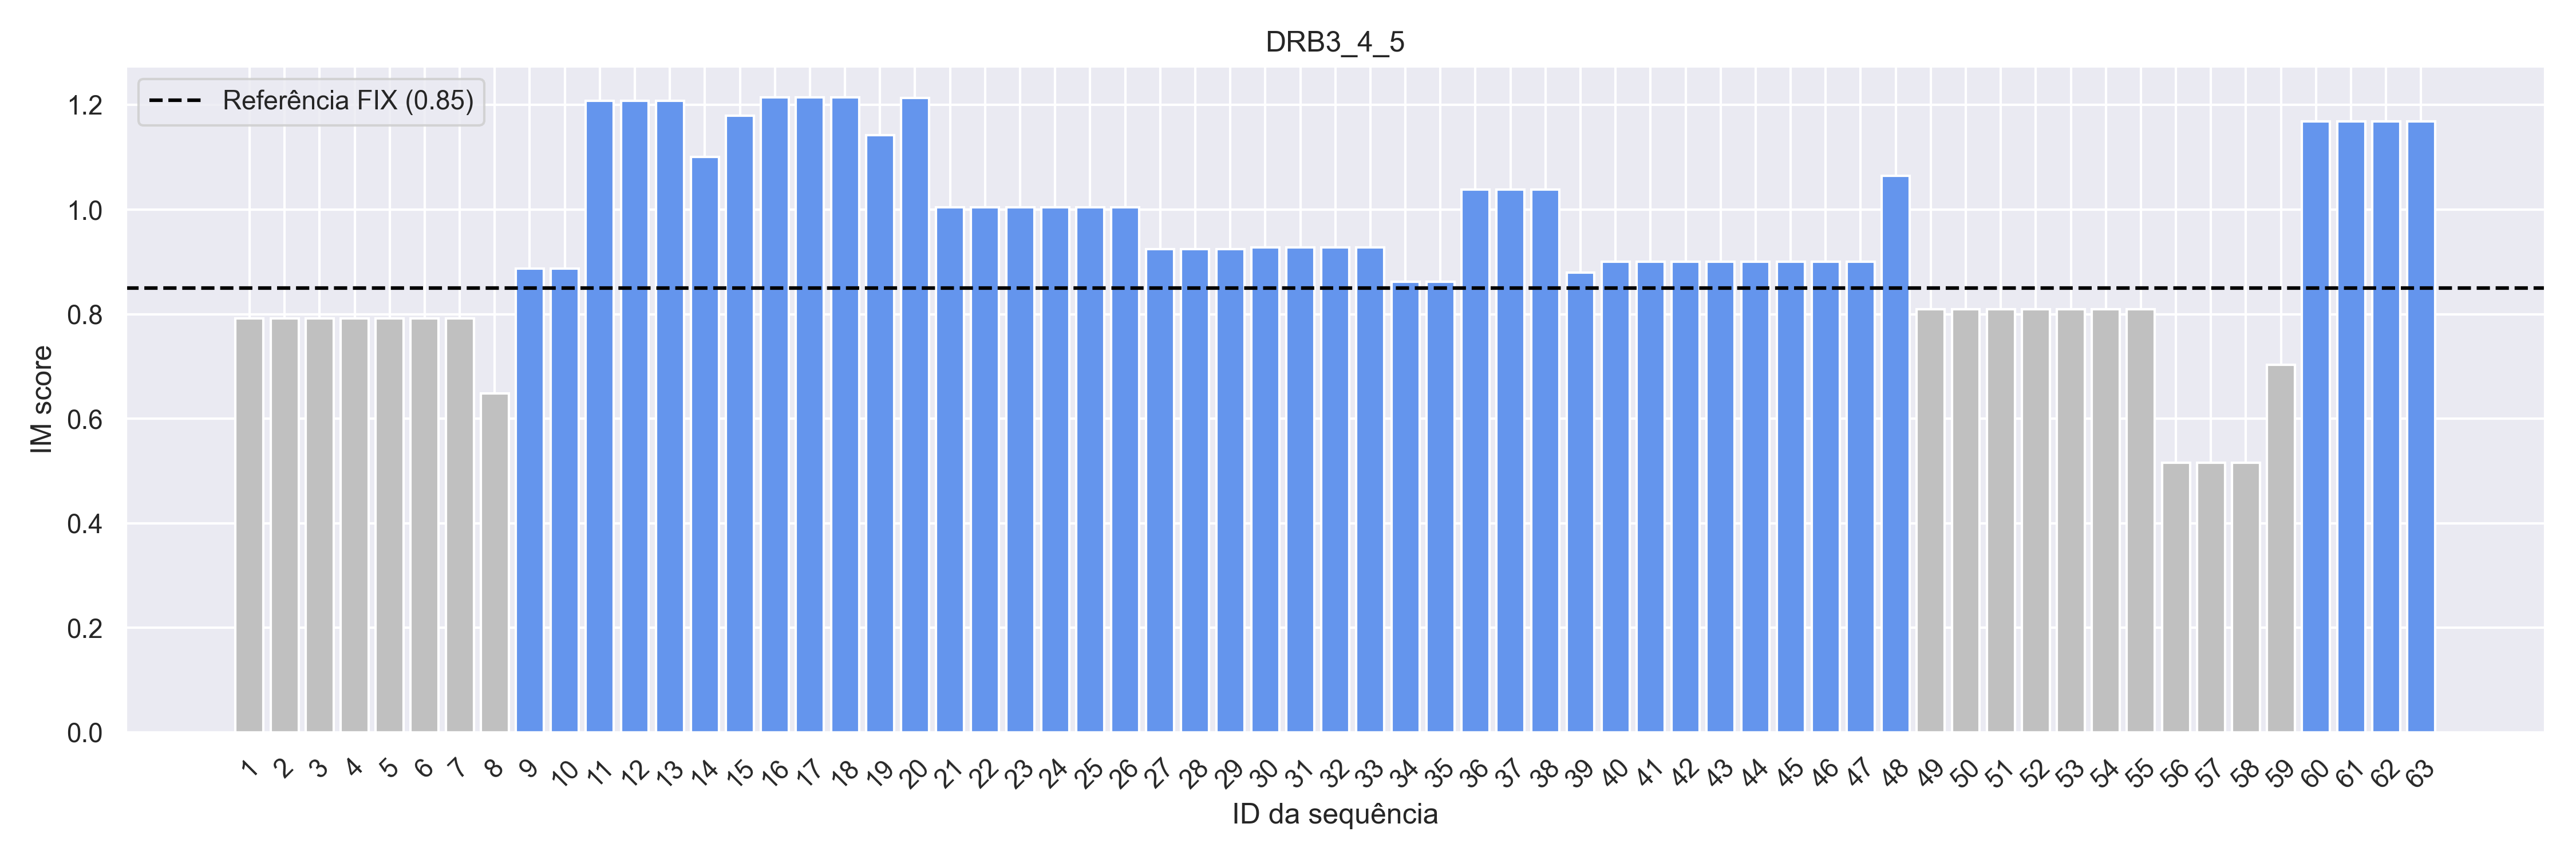
\includegraphics[width=\textwidth]{figuras/plot_imuno_IMscore_DRB3_4_5.png}
        %\caption{IM dos grupos DRB3, DRB4 e DRB5}
    \end{minipage} \\[1ex] %
    \begin{minipage}{0.9\textwidth}
        \centering
        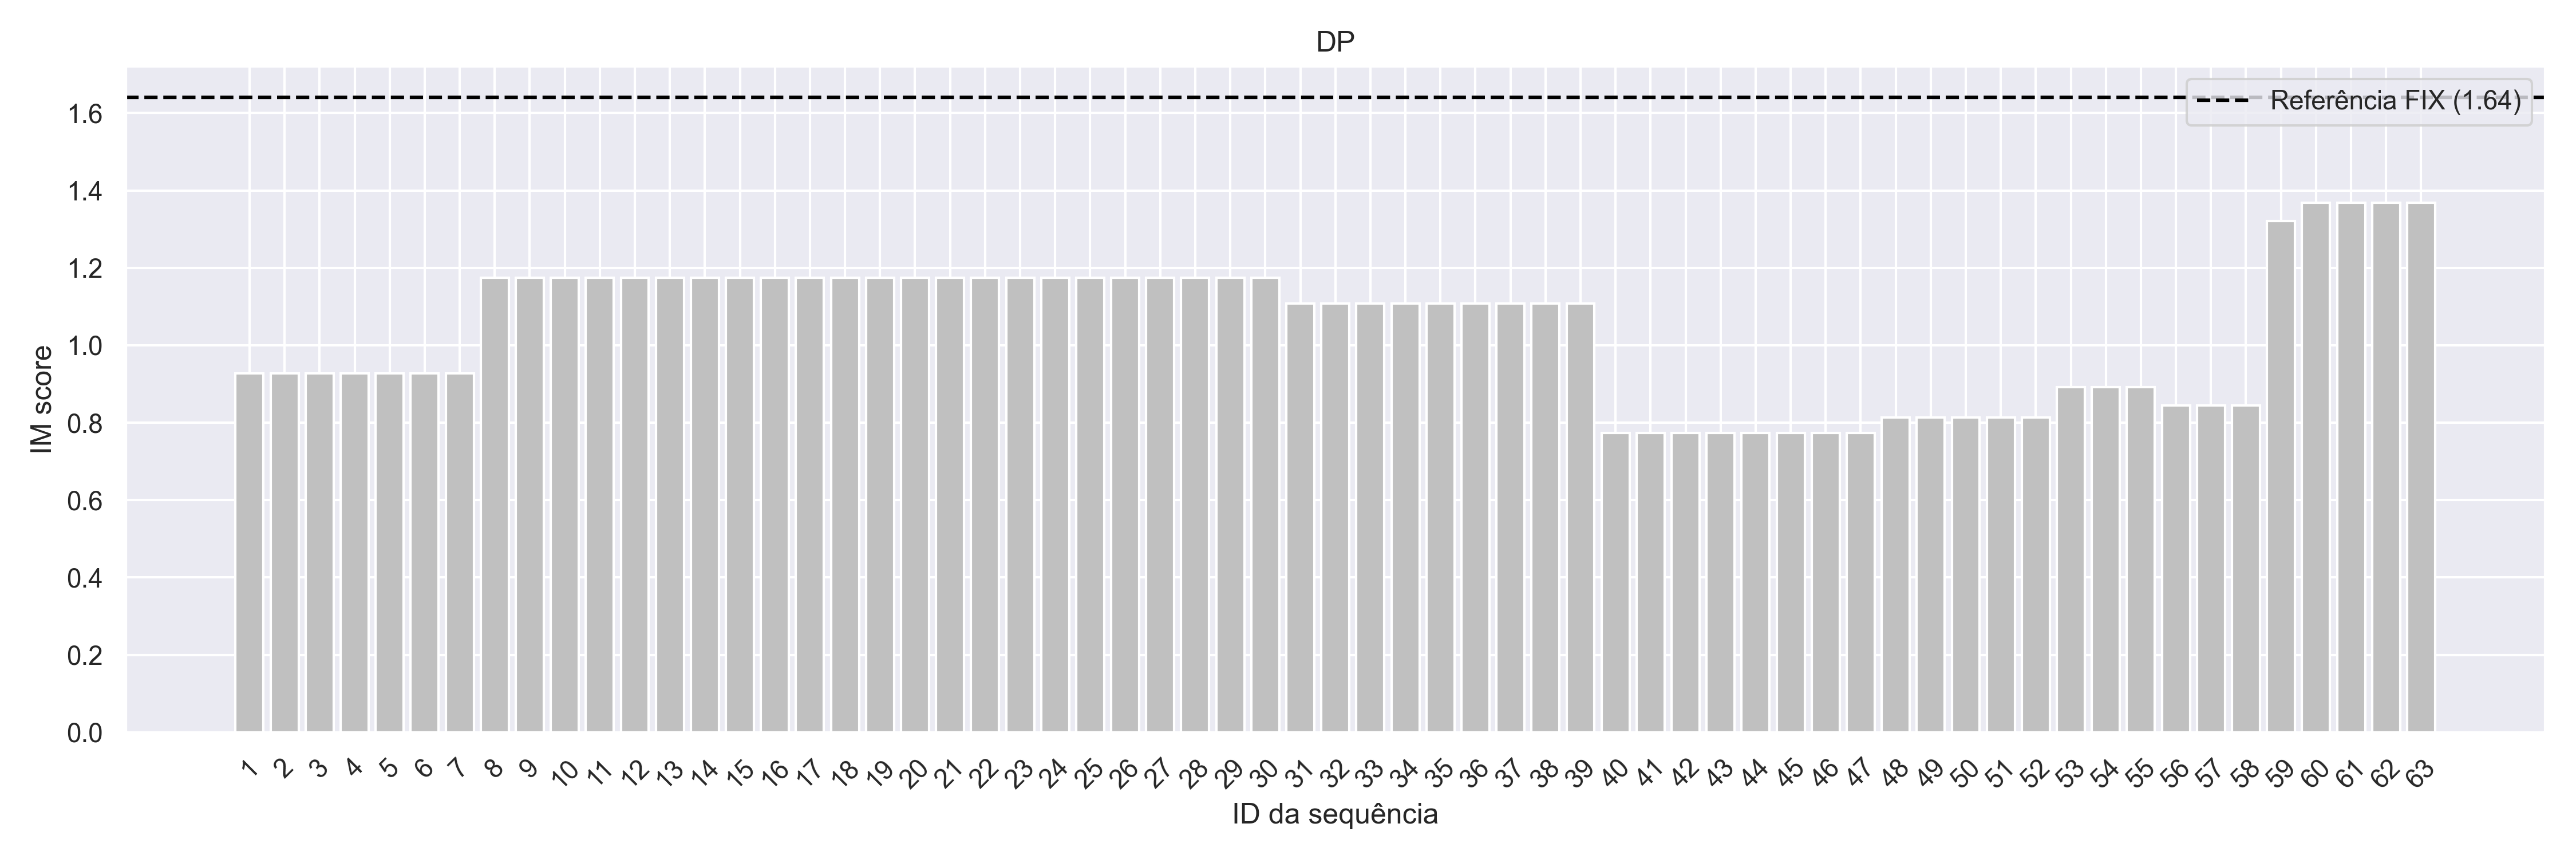
\includegraphics[width=\textwidth]{figuras/plot_imuno_IMscore_DP.png}
        %\caption{IM do grupo DP}
    \end{minipage} \\[1ex]%
    \begin{minipage}{0.9\textwidth}
        \centering
        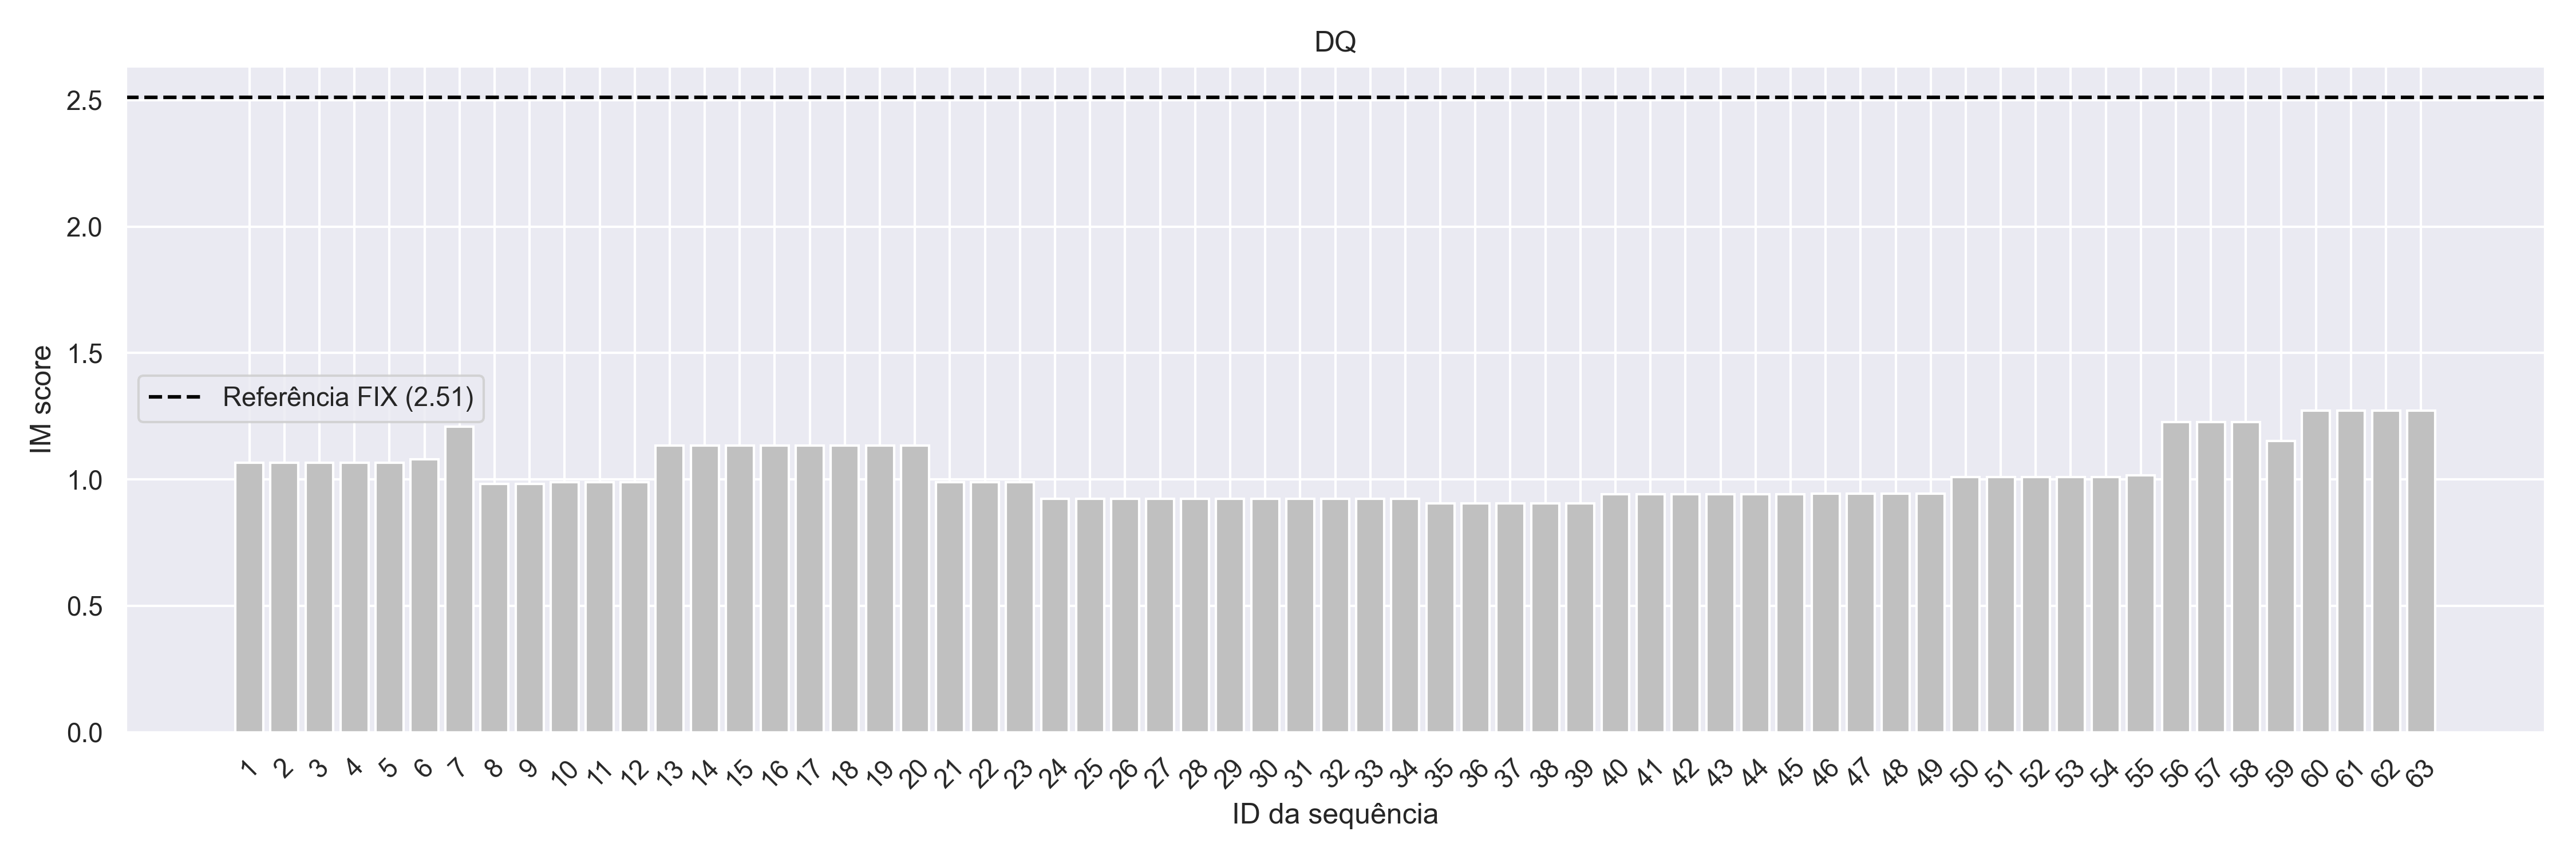
\includegraphics[width=\textwidth]{figuras/plot_imuno_IMscore_DQ.png}
        %\caption{IM do grupo DQ}
    \end{minipage} 
    \caption{IM calculado para cada grupo de alelo}
\end{figure}


\section{Docking}       

Ao projetar proteínas capazes de substituir o FIX no tratamento da Hemofilia B, um aspecto crítico é garantir que as 
proteínas geradas possuem uma interação eficaz ou até mais favorável com o FVIII se comparado ao FIX.
Para isto, realizamos análises de \textit{docking} molecular de cada sequência gerada com o FVIII,
calculando métricas que capturam diferentes características da interface proteína-proteína. 
Ilustramos a seguir os resultados obtidos para as métricas \textit{CMS}, \textit{IBSASA}, \textit{SAP Score} e \textit{DDG}.
Estão destacadas em azul as proteínas que superaram o FIX em cada métrica.
Em termos de \textit{CMS}, obtivemos 56 proteínas (89\% do total) superiores ao FIX, 
sugerindo interfaces de ligação maiores para essas sequências.
O \textit{DDG}, que mede a estabilidade da interação, indicou que 46 proteínas (73\% do total) 
são mais estáveis (DDG menor) do que o FIX.
O \textit{IBSASA}, que mede a área de superfície enterrada na interface, indicou que 51 proteínas (81\% do total)
foram superiores ao FIX.
Por fim, em termos de \textit{SAP Score}, praticamente todas as proteínas geradas obtiveram valores muito próximos ao 
calculado para o FIX, tendo 51 proteínas levemente mais favoráveis (81\% do total), i.e., formando complexos menos propensos à agregação.
Em geral, 30 proteínas (48\% do total) superaram o FIX em todas as métricas,
sugerindo que as proteínas geradas podem formar complexos eficientes com o FVIII.

\begin{figure}[H]
    \centering
    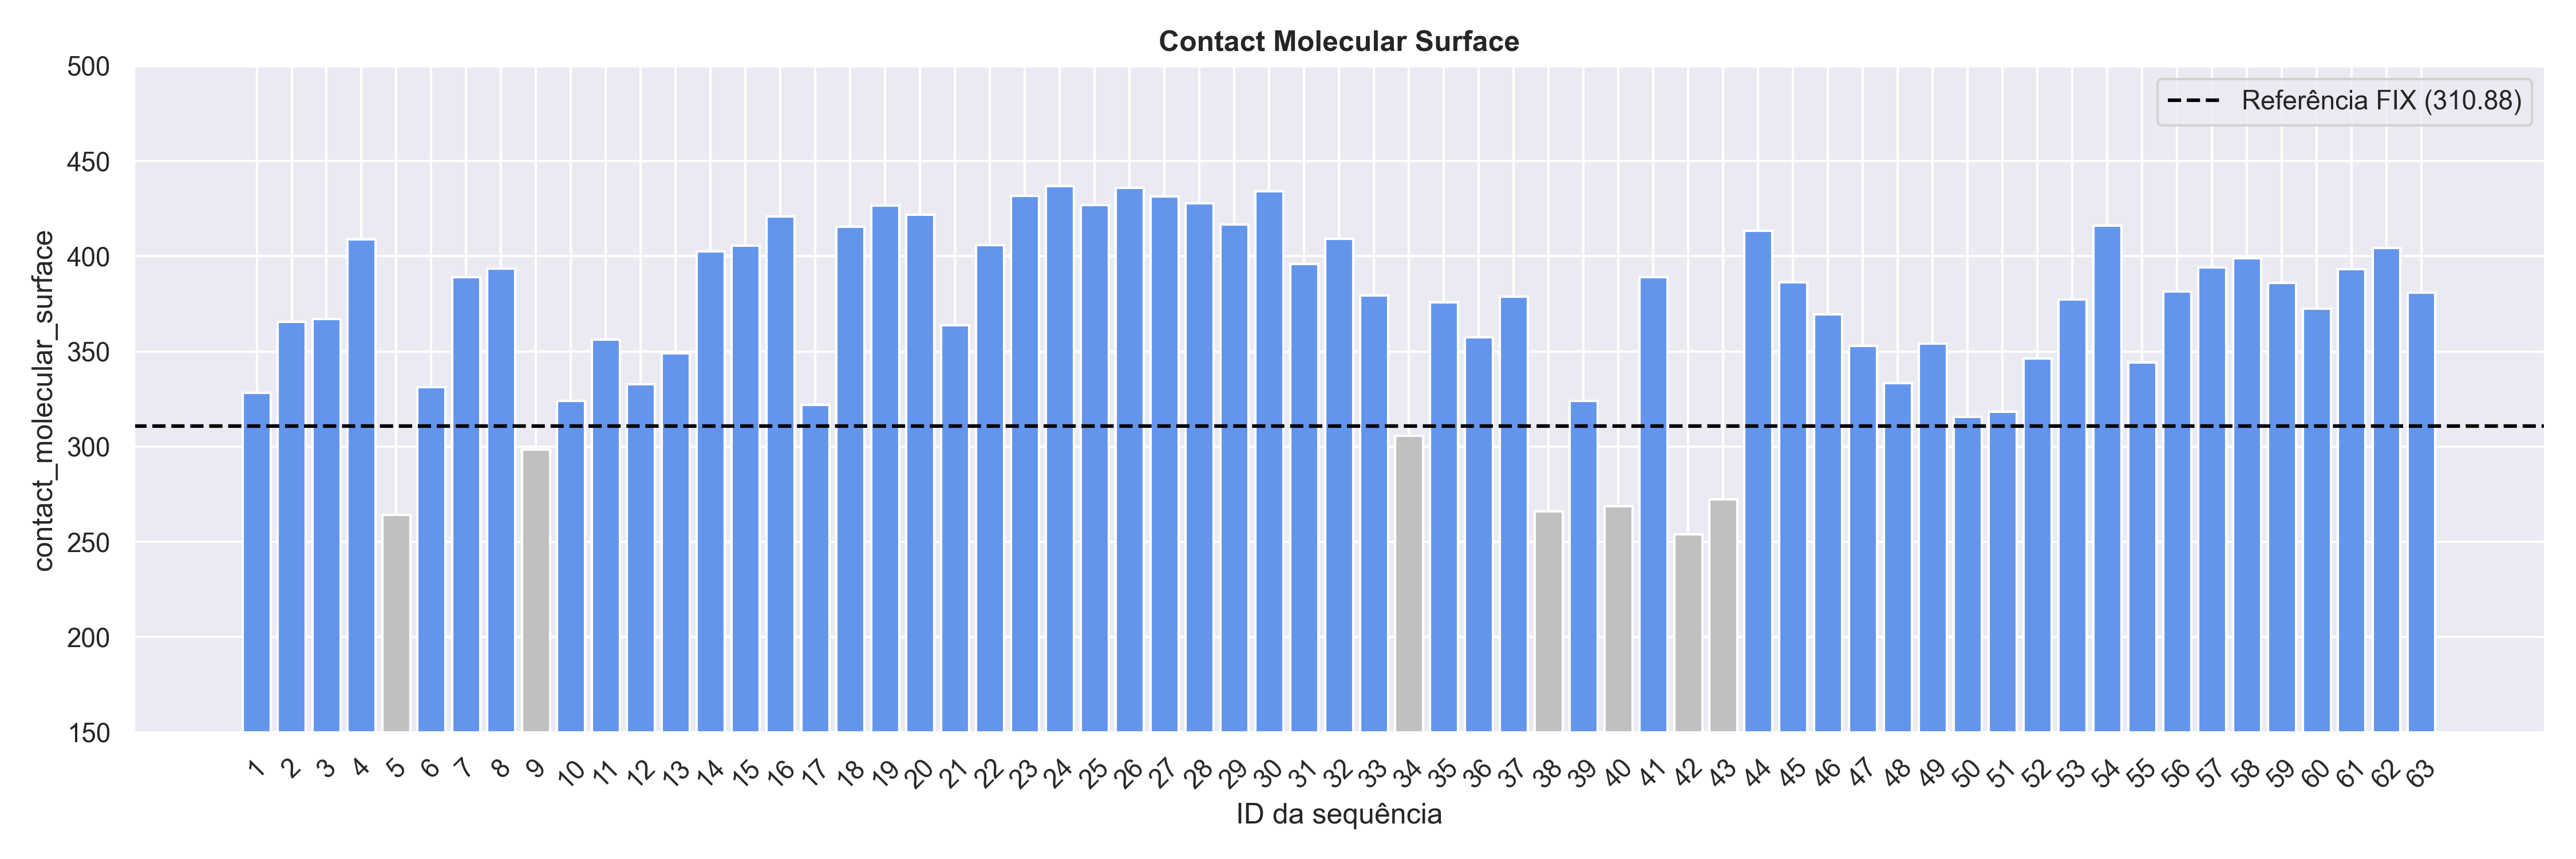
\includegraphics[width=.9\linewidth]{figuras/plot_contact_molecular_surface.png}    
    \caption{Resultado do \textit{CMS} entre as proteínas geradas e o fator VIII}
\end{figure}

\begin{figure}[H]
    \centering
    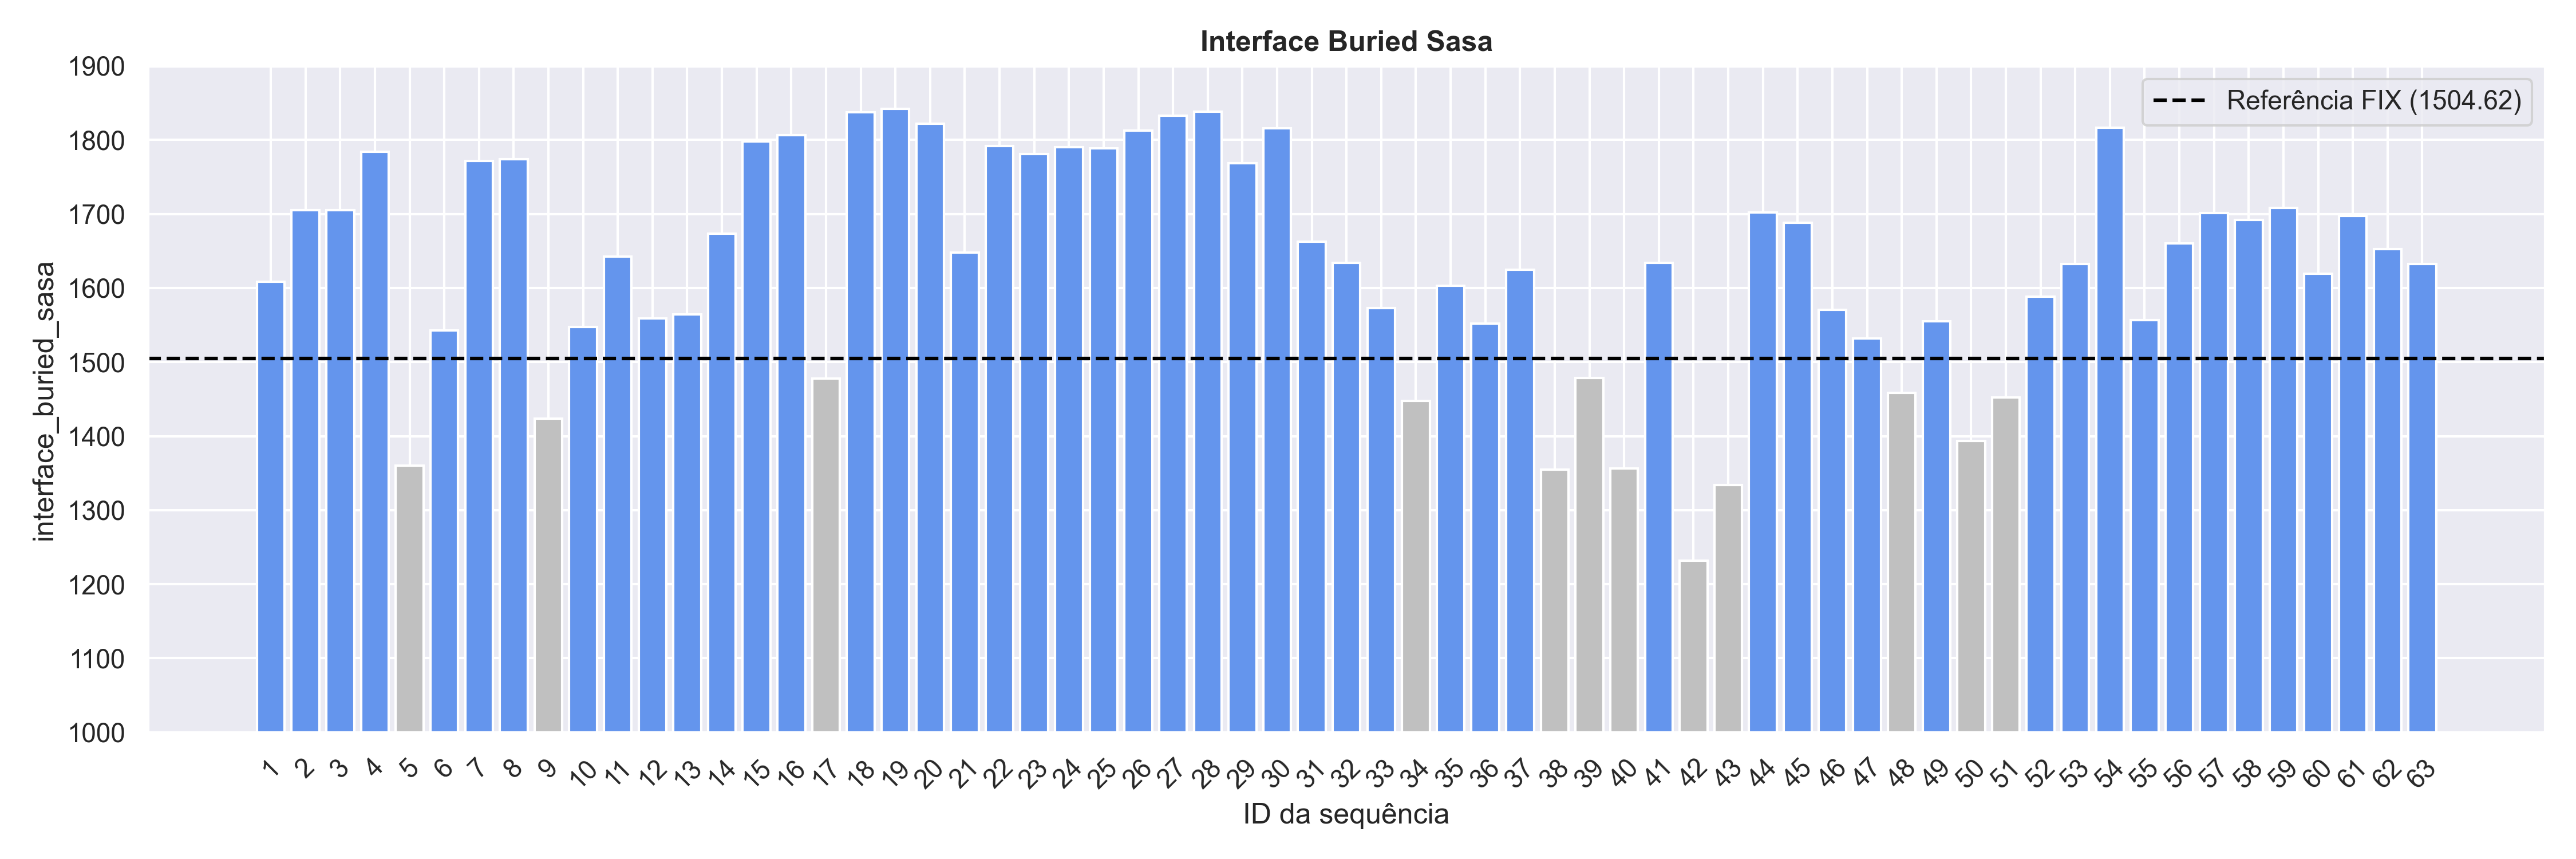
\includegraphics[width=.9\linewidth]{figuras/plot_interface_buried_sasa.png}    
    \caption{Resultado do \textit{IBSASA} entre as proteínas geradas e o fator VIII}
\end{figure}

\begin{figure}[H]
    \centering
    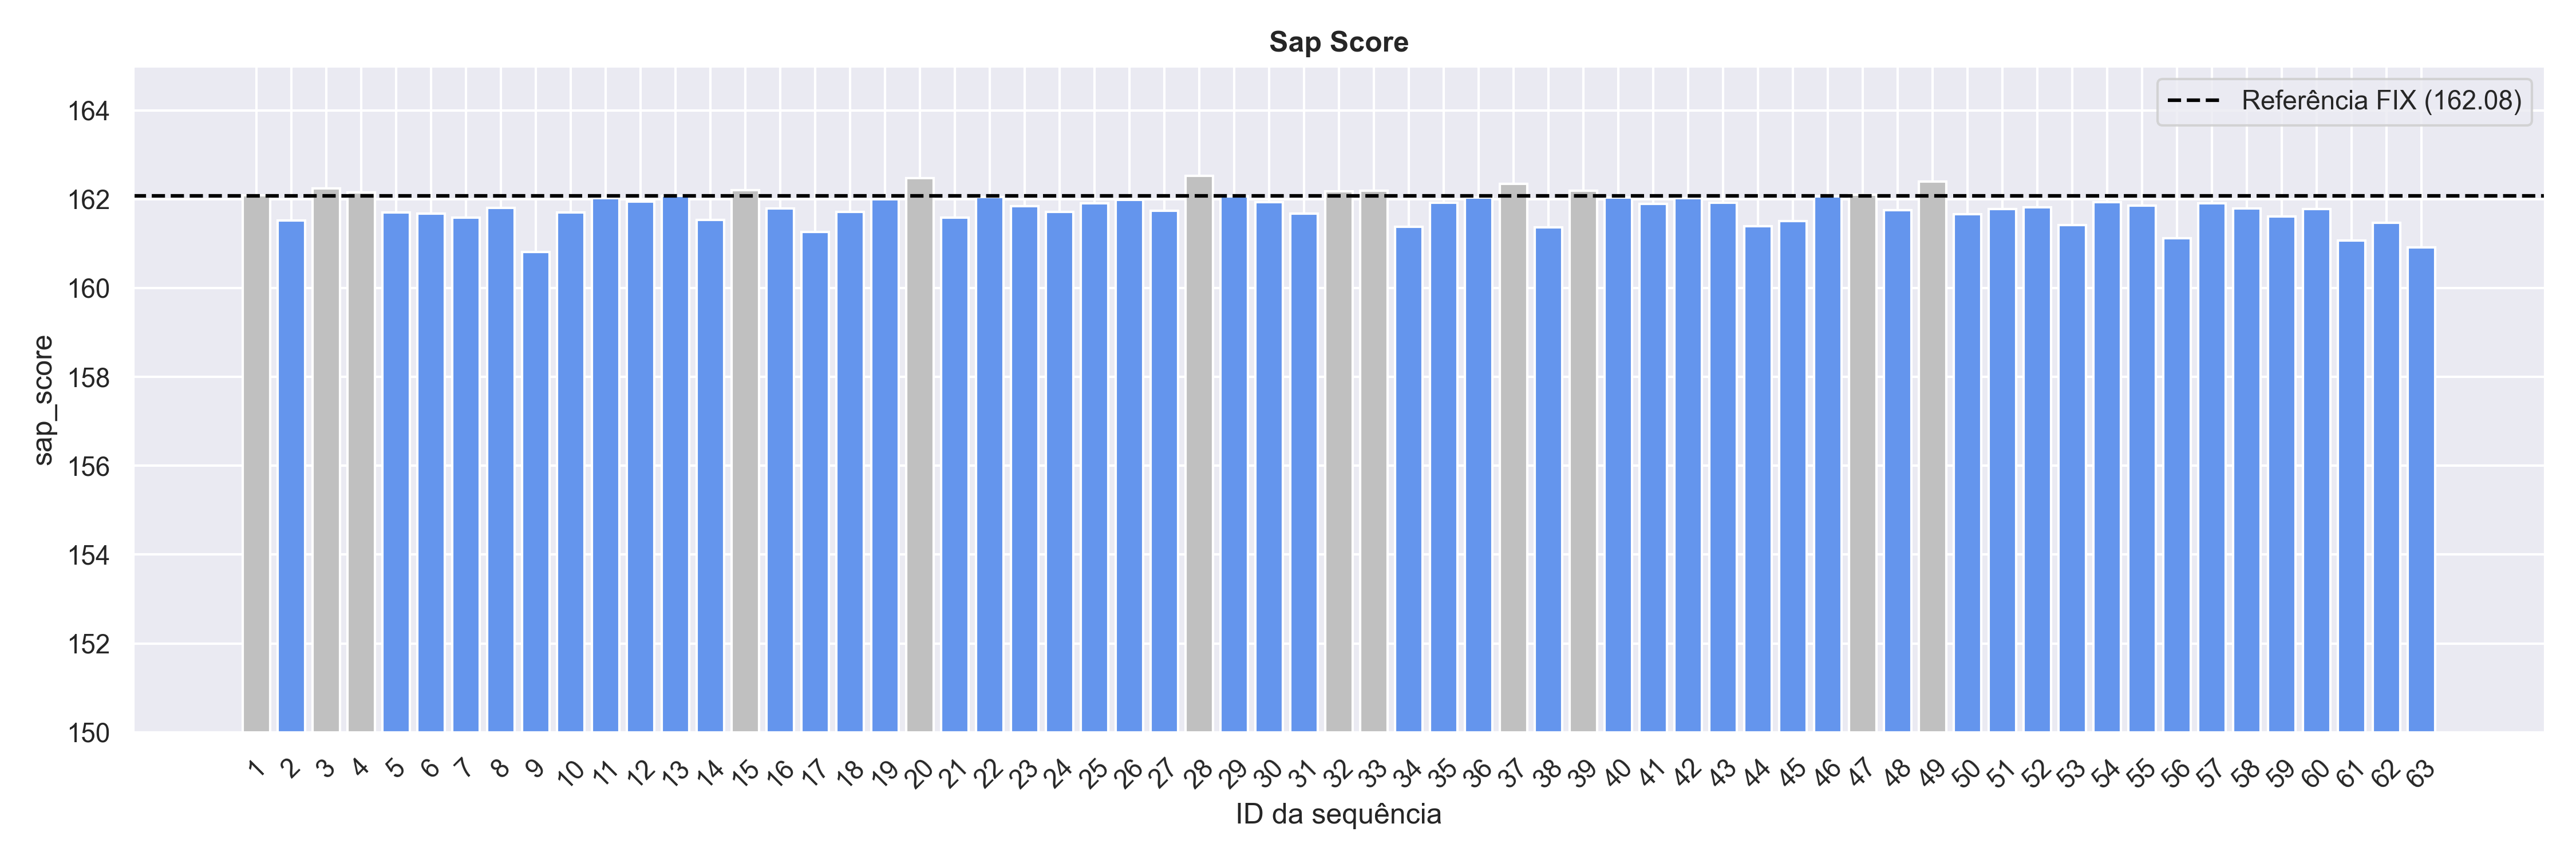
\includegraphics[width=.9\linewidth]{figuras/plot_sap_score.png}    
    \caption{Resultado do \textit{SAP Score} entre as proteínas geradas e o fator VIII}
\end{figure}

\begin{figure}[H]
    \centering
    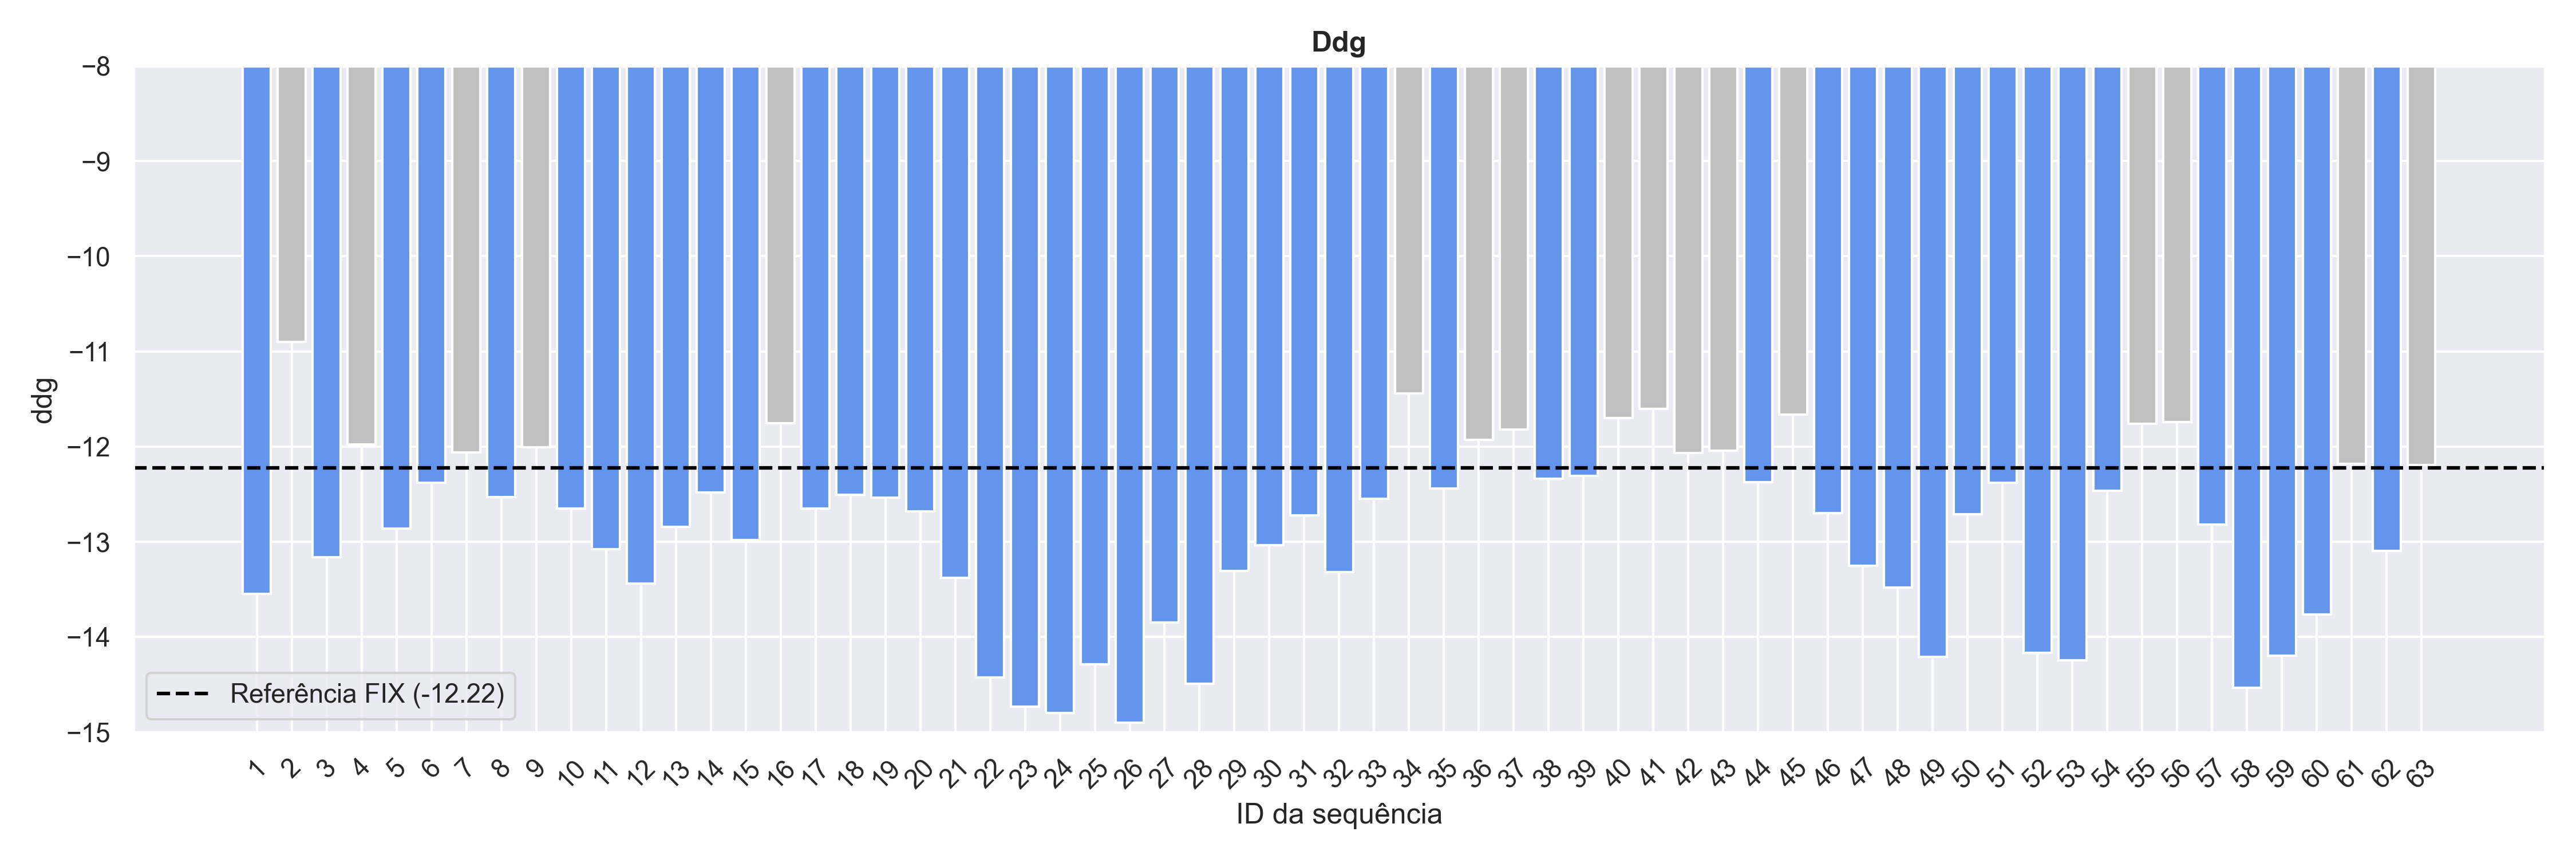
\includegraphics[width=.9\linewidth]{figuras/plot_ddg.png}    
    \caption{Resultado do \textit{DDG} entre as proteínas geradas e o fator VIII}
\end{figure}










\chapter{Conclusão}
{\color{red} Em andamento}


Este trabalho apresentou um novo paradigma para o \textit{design} de proteínas terapêuticas,
aplicando aprendizado por reforço profundo para otimizar a sequência do fator IX (FIX),
com o objetivo de melhorar sua estabilidade estrutural, 
reduzir a imunogenicidade e potencializar sua eficácia no tratamento da hemofilia tipo B.  

A abordagem proposta combinou metodologias avançadas de modelagem molecular e inteligência artificial 
para explorar de maneira eficiente o vasto espaço de sequências proteicas. 
O uso do algoritmo \textit{Proximal Policy Optimization} (PPO) permitiu a evolução de variantes do FIX 
por meio de um processo iterativo de seleção e refinamento, 
guiado por métricas estruturais e funcionais. 
A validação das proteínas geradas foi realizada por meio de análises computacionais, 
incluindo \textit{Template Modeling Score} (TM-Score), 
\textit{Contact Molecular Surface} (CMS) e \textit{docking} molecular com o Fator VIII (FVIII), 
demonstrando que algumas variantes apresentam potencial terapêutico promissor.  

A principal contribuição deste trabalho reside na aplicação inédita de aprendizado por reforço profundo
para a otimização do FIX, um campo ainda pouco explorado na literatura científica. 
A inexistência de estudos anteriores que utilizem essa abordagem para o design de proteínas 
voltadas ao tratamento da hemofilia B reforça a originalidade e a relevância deste estudo.  

Embora os resultados obtidos sejam promissores, 
este trabalho apresenta algumas limitações. 
A ausência de validação experimental (\textit{wet lab}) impede a confirmação direta 
da funcionalidade das proteínas geradas, 
sendo necessário realizar testes laboratoriais para avaliar sua estabilidade e atividade biológica. 
Além disso, futuras melhorias podem incluir a incorporação de simulações físicas
mais sofisticadas para refinar as predições estruturais e funcionais do modelo.  

Em síntese, este trabalho demonstra o potencial do aprendizado por reforço profundo no design racional
de proteínas terapêuticas. 
Os avanços obtidos aqui podem servir de base para novas pesquisas que busquem aprimorar o 
desenvolvimento de biofármacos personalizados, 
contribuindo para a inovação no tratamento da hemofilia tipo B e outras doenças genéticas.





%%%%%%%%%%%%%%%%%%%%%%%%%%%% APÊNDICES E ANEXOS %%%%%%%%%%%%%%%%%%%%%%%%%%%%%%%%

% Um apêndice é algum conteúdo adicional de sua autoria que faz parte e
% colabora com a ideia geral do texto mas que, por alguma razão, não precisa
% fazer parte da sequência do discurso; por exemplo, a demonstração de um
% teorema intermediário, as perguntas usadas em uma pesquisa qualitativa etc.
%
% Um anexo é um documento que não faz parte da tese (em geral, nem é de sua
% autoria) mas é relevante para o conteúdo; por exemplo, a especificação do
% padrão técnico ou a legislação que o trabalho discute, um artigo de jornal
% apresentando a percepção do público sobre o tema da tese etc.
%
% Os comandos appendix e annex reiniciam a numeração de capítulos e passam
% a numerá-los com letras. "annex" não faz parte de nenhuma classe padrão,
% foi criado para este modelo. Se o trabalho não tiver apêndices ou anexos,
% remova estas linhas.
%
% Diferentemente de \mainmatter, \backmatter etc., \appendix e \annex não
% forçam o início de uma nova página. Em geral isso não é importante, pois
% o comando seguinte costuma ser "\chapter", mas pode causar problemas com
% a formatação dos cabeçalhos. Assim, vamos forçar uma nova página antes
% de cada um deles.

%%%% Apêndices %%%%

\makeatletter
\if@openright\cleardoublepage\else\clearpage\fi
\makeatother

\pagestyle{appendix}

\appendix

% \addappheadtotoc acrescenta a palavra "Apêndice" ao sumário; se
% só há apêndices, sem anexos, provavelmente não é necessário.
\addappheadtotoc

%\input{conteudo/apendice-exemplo-pseudocodigo}
%\par

%%%% Anexos %%%%

\makeatletter
\if@openright\cleardoublepage\else\clearpage\fi
\makeatother

\pagestyle{appendix} % repete o anterior, caso você não use apêndices

\annex

% \addappheadtotoc acrescenta a palavra "Anexo" ao sumário; se
% só há anexos, sem apêndices, provavelmente não é necessário.
\addappheadtotoc

%\input{conteudo/anexo-exemplo-faq}
%\par


%%%%%%%%%%%%%%% SEÇÕES FINAIS (BIBLIOGRAFIA E ÍNDICE REMISSIVO) %%%%%%%%%%%%%%%%

% O comando backmatter desabilita a numeração de capítulos.
\backmatter

\pagestyle{backmatter}

% Espaço adicional no sumário antes das referências / índice remissivo
\addtocontents{toc}{\vspace{2\baselineskip plus .5\baselineskip minus .5\baselineskip}}

% A bibliografia é obrigatória

\printbibliography[
  title=\refname\label{bibliografia}, % "Referências", recomendado pela ABNT
  %title=\bibname\label{bibliografia}, % "Bibliografia"
  heading=bibintoc, % Inclui a bibliografia no sumário
]

%\printindex % imprime o índice remissivo no documento (opcional)

\end{document}
